%%
%% This is file `yanputhesis-sample.tex',
%% generated with the docstrip utility.
%%
%% The original source files were:
%%
%% yanputhesis.dtx  (with options: `sample')
%% Copyright (C) 2022 by Shangkun Shen
%% 
%% It may be distributed and/or modified under the conditions of the LaTeX
%% Project Public License, either version 1.3b of this license or (at your
%% option) any later version. The latest version of this license is in
%%     https://www.latex-project.org/lppl.txt
%% and version 1.3b or later is part of all distributions of LaTeX version
%% 2005/12/01 or later.
%%=============================================================================%
%% 设置论文格式(学位、盲评、Adobe 字体)
%%-----------------------------------------------------------------------------%
%% 博士、正常版本、不使用 Adobe 字体
%% \documentclass[lang=chs, degree=phd, blindreview=false, adobe=false]{yanputhesis}
%% 博士、盲评版本、不使用 Adobe 字体
%% \documentclass[lang=chs, degree=phd, blindreview=true, adobe=false]{yanputhesis}
%% 博士、正常版本、强制使用 Windows 系统字体
\documentclass[lang=chs, degree=master, blindreview=false, winfonts=true]{yanputhesis}
%% 硕士、正常版本、不使用 Adobe 字体
%% \documentclass[lang=chs, degree=master, blindreview=false, adobe=false]{yanputhesis}
%% 硕士、盲评版本、不使用 Adobe 字体
%% \documentclass[lang=chs, degree=master, blindreview=true, adobe=false]{yanputhesis}
%%=============================================================================%
%% 导言区:请自行添加额外宏包
%%-----------------------------------------------------------------------------%
\usepackage{blindtext}                                      % 生成无意义文本
\usepackage{metalogo}                                       % 软件标志
\usepackage[binary-units=true]{siunitx}                     % 物理量单位
\usepackage{amsmath}    
                                    % 基础数学库
\usepackage{bm}
%\usepackage{multirow}
%\usepackage{bbm}
%\usepackage{setspace}
\usepackage{graphicx}  %插入图片的宏包
\usepackage{float}  %设置图片浮动位置的宏包
%\usepackage{amssymb}
%\usepackage{amsthm}
\usepackage{amsfonts}
%\renewcommand{\qedsymbol}{\text{}}
\usepackage{caption}
\usepackage{subcaption}
\usepackage{algorithm}
\usepackage{algpseudocode}

% \renewcommand{\algorithmicrequire}{ \textbf{Input:}} %Use Input in the format of Algorithm
% \renewcommand{\algorithmicensure}{ \textbf{Output:}} %UseOutput in the format of Algorithm




%%=============================================================================%
%% 参考文献(也可以是独立文件)
%%-----------------------------------------------------------------------------%
\begin{filecontents}{reference.bib}

\end{filecontents}
%%=============================================================================%
%% 基本信息录入
%%-----------------------------------------------------------------------------%
\title{数据驱动下的无人机\\绳系吊运控制研究\\}{          % 中英文标题
A data-driven research on tethered hoisting \\ control of unmanned aerial vehicle (UAV)
}                                                           % 请自行断行
\author{\blackbox{李晨豪}}{\blackbox{Li Chenhao}}  % 姓名(添加盲评标记)
\date{2025年3月}{March 2025}                                  % 答辩日期
\school{航天学院}{School of Astronautics}% 学院
\major{控制科学与工程}{Control Science and Engineering}                     % 专业 博士请添加 Ph
\advisor{\blackbox{张帆}}{\blackbox{Zhang Fan}}      % 导师(添加盲评标记)
\studentnumber{\blackbox{2022200330}}                                  % 学号
%\funding{本研究得到玄学基金(编号23336666)资助。}{         % 基金资助
%    The present work is supported by Funding of Metaphysics %
%    (Project No:23336666).}                                %
%%=============================================================================%
%% 文档开始
%%-----------------------------------------------------------------------------%
\begin{document}
%%-----------------------------------------------------------------------------%
%% 总前言,包含封皮页、中英文标题、中英文摘要、目录
%%-----------------------------------------------------------------------------%
\frontmatter                                                % 前言部分
\maketitle                                                  % 封皮页及标题页
%-----------------------------------------------------------------------------%
\makeCommitteePage{                                         % 学位论文评阅人
    \reviewers{\fullBlindReview{1}}                         % 和答辩委员会名单
    
    \committee{2025 年 3 月 6 日}{
        \defenseChair{王志刚}{教授}{西北工业大学}
        \committeeMember{刘正雄}{教授}{西北工业大学}
        \committeeMember{常海涛}{副研究员}{西北工业大学}
        \defenseSecretary{沈刚辉}{副教授}{西北工业大学}
    }
}
%%-----------------------------------------------------------------------------%
\begin{abstract}                                            % 中文摘要开始
    凭借优异的垂直起降能力和高机动性,四旋翼无人机在军事和民用领域得到了广泛应用。在工业巡检和物流运输等领域中,利用四旋翼无人机开展空中吊运任务,不仅能够有效应对复杂的地面环境,还可以替代传统机械设备完成物资搬运和投放等工作。绳系无人机凭借其灵活性、通用性、简便性等优势,逐渐成为无人机运输领域的新兴研究热点。然而,由于无人机本身是一个欠驱动控制系统,加之携带载荷的系绳吊挂结构,使得其运动特性更加复杂。在多无人机系统中,吊挂载荷的质量、尺寸不都是完全规则的,系统内不确定系绳拉力对无人机稳定飞行造成影响。因此,无人机绳系吊运系统的稳定控制是一个值得研究的具有挑战性的复杂问题。
    
近年来,数据驱动方法因其能够避免复杂系统高昂的建模成本、适应未知环境和动态变化、实现自主优化等特点,逐渐成为控制领域的重要方法。与传统的基于模型的控制方法相比,数据驱动控制不依赖精确的物理模型,能够直接从数据中学习控制策略,具有更强的适应性、灵活性和优化能力,特别适用于复杂、高维、不确定或动态变化的系统。

本文将探讨数据驱动控制在无人机绳系吊运系统中的应用,重点研究单无人机吊装载荷的高精度跟踪与多无人机协同稳定控制问题,并通过物理引擎仿真和试验验证其有效性。基于以上研究框架,本文的具体研究内容如下:

首先推导了无人机绳系吊运系统的动力学模型。从单个无人机出发,基于牛顿-欧拉法建立了单个四旋翼无人机的动力学方程,并通过拉格朗日法推导出了单个无人机吊装载荷的混合动力学模型并进行了简化。对于多无人机绳系吊运系统,基于拉格朗日法方程求解了系统的动力学模型,并推导了在载荷状态未知情况下的简化动力学模型。

针对单无人机吊装载荷中的不确定非线性项干扰问题,提出了一种基于数据驱动的控制框架,用于四旋翼无人机在激进飞行条件下的绳系吊挂载荷控制。受Koopman算子理论启发,设计损失函数并通过深度神经网络进行学习,将有效载荷及无人机自身空气动力产生的力和扭矩建模为一个升维的显式线性动力系统,并通过Lipschitz常数从理论上保证了预测误差的界限,显着提高了预测模型的准确性;将学习得到的动力学模型与无人机的名义动力学系统相结合形成了完整的系统模型,并应用到非线性模型预测控制框架中,验证了方案的有效性。

为了实现多无人机协同吊装系统的稳定控制,结合上述数据驱动的模型预测控制,自动调整系统的模型预测控制器并解决各无人机系绳上拉力分配问题。开发了一种分布式策略梯度算法。采用多层感知网络在线生成自适应归一化超参数,以闭环方式有效地训练这些深度神经网络,直接从轨迹跟踪误差中学习自适应模型预测控制的权重,提高了系统训练时的稳定性和跟踪性能;通过分析系绳上的张力,在多无人机协同吊装系统数据驱动控制方法的基础上通过自适应调整权重参数,确保系绳拉力以最优方式分配,在保持系统稳定的同时对编队构型进行优化。

最后,搭建了无人机绳系吊运系统的物理引擎仿真平台和实物试验平台对算法进行了验证。在仿真中,通过多种开源物理引擎对系统进行建模并进行了对比,结果表明,设计的数据驱动控制算法能够有效实现系统对期望轨迹的精确跟踪;在实物试验中,提出了系统的总体设计方案,并进一步细化了器件选型和机构设计,试验结果也验证了算法的有效性。

综上所述,本文对无人机绳系吊运载荷进行了全面的研究,建立了单无人机和多无人机系统的动力学模型,对模型进行了进一步简化;利用了数据驱动方法对单无人机吊装载荷的不确定非线性项干扰进行预测,并补偿到非线性模型预测控制中;设计了一种基于数据驱动的神经网络学习自适应参数,并结合基于优化的系绳拉力分配方法用于多无人机协同吊装搬运系统的稳定控制;搭建了多个物理引擎和真实试验并对所提出算法进行了验证。

    
    \begin{keywords}                                        % 中文关键词开始
        无人机运输 ,  数据驱动控制, 模型预测控制, 模型自适应控制  , 物理引擎与试验                   %
    \end{keywords}                                          % 中文关键词结束
\end{abstract}                                              % 中文摘要结束
%%-----------------------------------------------------------------------------%
\begin{engabstract}                                         
	Unmanned aerial vehicles (UAVs), known for their excellent vertical take-off and landing capabilities and high maneuverability, are widely used in both military and civilian applications. In industrial inspection and logistics, these UAVs are employed for aerial lifting tasks. They can efficiently handle complex ground environments and replace traditional mechanical equipment for material transport and delivery. Tethered-UAV systems, with their flexibility, versatility, and simplicity, have gradually become a hot research topic in the field of UAV transportation research. However, UAVs are inherently underactuated systems, and the addition of a tethered load complicates their motion characteristics. In multi-UAV systems, the mass and size of the suspended payload are not all completely regular, and the uncertainty of the tether pull within the system has an impact on the stable flight of the UAV. Therefore, stabilizing the control of tethered-UAV systems is a complex and challenging problem that warrants further investigation.
		
	In recent years, data-driven methods have become a key approach in control systems. They offer advantages such as avoiding the high cost of modeling complex systems, adapting to unknown environments, and enabling autonomous optimization. Unlike traditional model-based control methods, data-driven control does not rely on precise physical models. It learns control strategies directly from data. This approach offers better adaptability, flexibility, and optimization. It is especially suitable for complex, high-dimensional, uncertain, or dynamically changing systems.
	
	This paper explores the application of data-driven control in tethered-UAV systems. It focuses on high-precision tracking for a single tethered-UAV systems and the cooperative stabilization control for multi-tethered-UAV systems. The effectiveness of the proposed methods is verified through both physics engine simulations and real-world experiments. Based on the above research framework, the specific research content of this paper is as follows:
	
	First, the dynamic model of the tethered-UAV system is derived. Starting from a single UAV, he kinetic equations of the single UAV are developed based on the Newton-Euler method, and a hybrid kinetic model for a single tethered-UAV systems is derived and simplified by the Lagrange method. For multi-tethered-UAV systems, the dynamics model of the system is modeled based on the Lagrange method, and a simplified dynamics model is derived for the case where the payload state is unknown.
	
	A data-driven control framework based on the uncertain nonlinear term interference problem in single tethered-UAV systems is proposed for tethered-UAV systems control of a UAV under aggressive flight conditions. Inspired by the Koopman operator theory, we design a loss function and use a deep neural network to model the forces and torques generated by the payload and the UAV's aerodynamic forces. This model is treated as an explicit lifted linear system in elevated dimensions. The Lipschitz constant is theoretically employed to bound the prediction error, significantly improving the accuracy of the model. The learned dynamical model is combined with the UAV's nominal dynamical system to form a complete system model. This model is then applied within a nonlinear model predictive control framework to verify the scheme's effectiveness.
	
	In order to realize the stabilization control of multi-tethered-UAV systems, the data-driven model predictive control described above is combined to automatically adjust the model predictive control parameters of the system and to solve the problem of tension distribution on the tethers of each UAV. A distributed strategy gradient algorithm is developed. Adaptive normalized hyperparameters are generated online using multilayer perceptual networks, and these deep neural networks are effectively trained in a closed-loop manner to learn the weights of adaptive model predictive control directly from the trajectory tracking error, which improves the stability and tracking performance of the system during training. By analyzing the tension on the tether, the formation configuration is optimized by adaptively adjusting the weight parameters on the basis of the data-driven control method of multi-tethered-UAV systems to ensure that the tether tension is distributed in an optimal way, while maintaining system stability.
	
	
	Finally, a physical engine simulation and real-world experiments of tethered-UAV systems are built to verify the algorithm. In the simulation, the system is modeled and compared by a variety of open-source physics engines, and the results show that the designed data-driven control algorithm can effectively realize the system's accurate tracking of the desired trajectory. In the real-world experiments, the overall design scheme of the system is proposed and the device selection and mechanism design are further refined. Test results validate the effectiveness of the algorithm.
	
	In conclusion, this paper provides a comprehensive study of the tethered-UAV system. The dynamical models for both single tethered-UAV systems and multi-tethered-UAV systems are established and further simplified. A data-driven approach is used to predict the uncertain nonlinear disturbances in a single tethered-UAV systems, which are then compensated in the nonlinear model predictive control. An adaptive parameter learning method based on a data-driven neural network is designed, combined with an optimization-based tether tension distribution method, for the stable control of multi-tethered-UAV systems. Multiple physical engine simulations and real-world experiments are carried out to validate the proposed algorithm.
	
   
   
    \begin{engkeywords}                                     % 英文关键词开始
        UAV Transportation \ensep Data-driven Control \ensep Model Predictive Control \ensep Model Reference Adaptive Control \ensep Physics Engine and Experiments         %
    \end{engkeywords}                                       % 英文关键词结束
\end{engabstract}                                           % 英文摘要结束
%%-----------------------------------------------------------------------------%
\tableofcontents                                            % 目录
%\listoffigures                                              % 图目录(学校未做要求)
%\listoftables                                               % 表目录(学校未做要求)
%\printnomenclature                                          % 符号表(学校未做要求)
%%-----------------------------------------------------------------------------%
\mainmatter
\sDefault

\chapter{绪论}
\chaptermark{绪论}
\section{课题研究背景及意义}
随着空中机器人领域的快速发展,作为一种可以自由漂浮的操纵器,四旋翼无人机(UAV,Unmanned Aerial Vehicle) 受到了人们的广泛关注,并在各个方面迅速普及\cite{kimon_advances_2023}。四旋翼无人机具有垂直起降能力,在空中还可以实现全方位的机动,已经被证明可以对城市进行探索和测绘\cite{tomic2012toward}、空中操纵物体\cite{suarez2020benchmarks}以及平衡和空翻等杂技表演\cite{beul2018fast},同时还可用于快递派送\cite{刘昂2020基于}、森林防火检测\cite{harikumar2018multi}、河流搜索\cite{nuske2015autonomous}、空中运输\cite{klausen2018cooperative},在军事和民用中都有着广泛的应用前景。

在短距离应急抢修作业中,滑坡中断道路、复杂地形地貌下导致物资运输车辆无法通行是灾害发生后应急抢修的重要阻碍,空中运输速度快、效率高,是解决复杂山区地形应急运输的有效方式之一。相比于直升机作业成本高、受限条件多、准备时间长、使用风险高等不利因素,四旋翼无人机作为简便、灵活的小型航空器具,不受限于仓位尺寸、便于多平台起降、可变构型避障、可多次灵巧往返/停靠于补给站点和孤立单位之间,在复杂地形进行应急抢修作业中具有无可比拟的优势。通过执行抓取、运输等操纵任务,其能够有效解决“最后一公里”物资运输和抢险救灾等问题。

物资运输已成为四旋翼无人机的一项热门应用\cite{cruz2014autonomous},对于无人机来说,在其对目标载荷进行运输时,可以采用不同的方法,配备额外的机构例如夹具、操纵器或绳系吊运系统等。使用夹具可以将载荷固连在无人机机体机腹或机体下方,该方法简单直接,使载荷保持在接近无人机重心的位置,有利于提高稳定性,但对目标载荷的形状和尺寸有着严格的约束,也会增加整个系统的惯性,使其功能仅限于执行慢速运动\cite{Khalifa2017};还可以在机体上挂载操纵器如机械臂、飞爪等刚性体,操作操纵器对目标载荷进行抓取,以实现无人机与外界环境的交互,但加装操纵器不仅造价昂贵,影响无人机的空气动力学特性,同时操纵器与无人机耦合严重,对作业时的稳定飞行控制提出了很高的要求;第三种方式绳系吊运系统就是将目标载荷直接通过柔性系绳挂载在机身下方,与前两种运输方式相比,采用柔性系绳连接目标载荷时不需要考虑运输载荷的形状和大小,其可以适应不同载荷的变化,避免了加装固定载荷的装置,使无人机的灵活性得以保留,增加了吊运的通用性。

系绳吊运载荷运输最初是为紧急响应、救援任务、民用和军事行动中的人力操作直升机而研究的\cite{2020A}。无人机绳系吊运载荷相比其它方法来说有着一系列的优越性,但随之而来的载荷也对无人机产生了一系列的影响。无人机绳系吊运系统是欠驱动和非线性耦合的,此外每个四旋翼无人机的动力学为载荷的摆动运动会引发无人机系统的不稳定性,同时给无人机系统增添了更多的自由度,使得此类系统的控制更具挑战性。

在运输过程中,单无人机在利用吊装方式运输的时候载荷会存在摆动,且当需要运输的载荷重量与无人机系统的载荷重量相当时,任务可能会受到影响。为了解决这些问题,采用多个协作式的无人机绳系吊运系统是一个很有前途的替代方案,即将多架无人机按照期望的队形来分布,并使其在执行任务的过程中保持编队队形平稳飞行,从而圆满完成运输任务。多无人机绳系吊运系统通过根据有效载荷重量适当调整四旋翼无人机的数量,使这种悬挂式有效载荷配置能够实现最大的有效载荷输送效率,此外这种配置还可以有效控制载荷的姿态,解决了单无人机运输载荷出现摆动的问题,甚至在单无人机发生故障时仍可以完成任务需求。因此多无人机吊运载荷具有可行性高、效率高以及扩展性强等单架无人机无法比拟的优势。但是,在依靠多无人机绳系吊运系统执行合作运输任务时,必须考虑一系列全新的因素。整个系统不仅受到载荷摆动的影响,而且还受到其它无人机运动的影响,如果单无人机的独立行动没有得到适当的协调,情况会变得更加复杂。

基于以上问题,本研究拟采用数据驱动方法来研究无人机绳系吊运系统,通过神经网络和无人机的动力学对整个系统进行动力学建模,提出了在线自适应神经元和模型预测控制相结合的控制算法对系绳的摆动进行抑制,在多无人机协同吊运中实现各个无人机功率消耗的均衡化,最终达到对搬运载荷的位姿的控制,有效提高系统的鲁棒性和安全性,为跨越峡谷、陡坡、滑坡体等障碍进行物资运输提供便捷、有效的手段,大大提高应急抢修作业效率,具有重要的应用价值。

\section{国内外研究现状}
\subsection{单无人机绳系吊装载荷控制研究现状}
多旋翼无人机(UAV)运输载荷主要通过固连、刚性连接或柔性连接的方式来进行。无人机绳系吊运具有方便、高效、节省土地资源、不受地形条件影响等优点,因此得到了广泛的应用。大疆今年发布的FlyCart30无人机也加入了空吊系统来实现无接触精准运送。然而,无人机绳系吊运也给控制研究带来了新的挑战,特别是载荷摆动对控制精度的降低,因此对于绳系连接载荷中的无人机在载荷干扰下实现高精度轨迹跟踪控制仍然是一个难点。目前,主要有两种方法解决该问题:一种是将重物视为扰动,并在控制器中对扰动量进行补偿;另一种是利用系统的摆动敏捷性,对无人机绳系吊装载荷系统整体进行建模,设计带有吊装载荷系统的四旋翼无人机的控制器。

对于无人机绳系吊装系统的建模方法,文献 \ref{yibo2013modeling} 假设系留综合缆绳的重力与所受风力作用于综合缆绳中心,且不考虑缆绳的拉伸变形,系留缆绳在自身重力、风的作用下呈现悬链线形状,可以求出无人机在不同位置时缆绳与机体的夹角。文献\ref{liu2020modeling}基于珠点模型对水下系留无人机进行建模。文献\ref{nicotra2017nonlinear}在假设缆绳不可拉伸、质量和阻尼可以忽略且具有零剪切刚度的前提下,通过分析二维平面上的无人机与系绳的运动学和动力学关系推导出系绳上的拉力。文献\ref{ferreira2015modeling}在建立旋翼无人机的动力学模型之后,将系绳建模成无质量的,由一个阻尼单元和一个弹簧单元并联,这两个并联单元再与一个弹簧单元串联的结构。文献 \ref{williams2006periodic} 将系绳建模为一系列通过非弹性杆连接的点质量块,通过分析这些杆件的动力学特性并进行仿真, 可以体现系绳的柔性。

对于设计带有绳系吊装系统的无人机的控制器方法,卡耐基梅隆大学的Sceenath得到了定义在构型空间SE ( 3 ) × S2上的坐标自由动力学模型,并将其可以看作平坦输出的微分平坦混合系统,并给出了控制器设计的稳定性证明和仿真\ref{sreenath2013geometric}。华盛顿大学的Lee团队提出了基于拉格朗日动力学在流形上的吊装载荷,将柔性电缆用串行连接的链路进行建模,并用几何非线性控制渐近稳定无人机的位置\ref{goodarzi2015geometric}。墨西哥的Guerrero提出最小化吊装载荷的摆动角度,以实现稳定\ref{guerrero2015passivity}。香港科技大学的沈劭劼团队设计了一种具有分层扰动补偿策略的自适应NMPC来克服未知外部扰动和模型参数不准确的问题\ref{li2023autotrans}。


\subsection{多无人机绳系吊装载荷运输研究现状}
为了适用于多样的载荷类型,系绳连接的多无人机协同运输方式也被学者们提出。早在 2011 年,Vijay Kumar 教授团队就根据多无人机绳系运输系统与绳驱并联操作机器人的相似性,将绳驱并联操作机器人的控制方法拓展到多无人机绳系运输系统上,对系统精确建模,根据载荷的期望位姿和几何约束,进行逆运动学求解,从而反解出每个无人机期望位置,完成载荷的控制\ref{michael2011cooperative}。Lee 使用利用拉格朗日方程的方法对系统建模,使用几何控制的方法,实现了对刚体载荷的精确位姿控制。文献\ref{cardona2019cooperative}使用了牛顿-欧拉法对系统建模,应用了将机械手多指抓取中的零交互力条件,设计了基于位置的被动控制。文献\ref{shirani2019cooperative}则是使用了上个世纪 90 年代提出的 Udwadia–Kalaba 方程\ref{udwadia1996equations},可以较为简单的针对多无人机绳系吊运这样的多约束系统求解出其动力学模型,最后应用了 LQR 控制。

以上文献中,由于载荷的存在,默认飞行过程中的系统模型是连续的(即假设绳始终有张力,载荷始终受力,不存在自由落体运动),系统中系绳模型都是作为无质量杆来处理。文献 \ref{gimenez2018multi }考虑了两架直升机协同运输一个载荷,较为不同的是绳子模型为多弹簧阻尼的柔性模型。文献\ref{masone2016cooperative}也从绳驱并联操作机器人受到启发,通过柔性模型考虑了协同运输中绳上的力分配问题。Tognon 教授团队考虑了系统建模中的不确定问题和无人机与载荷的多连接情形\ref{sanalitro2020full}。Erskine 团队首先研究了不同无人机期望角度构型下的系统载荷能力\ref{erskine2019control},在此基础上还研究了可变绳长的多无人机协同运输系统的载荷控制问题\ref{li2020design}。


\subsection{数据驱动控制研究现状}
使用自主机器人进行快速灵活的机动操作,需要了解平台的精确动力学模型。然而,对于刚柔混合的无人机绳系吊装系统,由于摩擦、空气动力学、绳子上的力突变造成的影响,传统的动力学模型并不总能捕捉到完整的系统行为。因此,在控制无人机时需要在模型的可表达性和计算的可操作性之间找到一个平衡点。随着系统越来越复杂,数据越来越容易获得,很多研究人员开始绕过经典的基于模型的技术,转而采用数据驱动的方法\ref{hou2013model},而无模型和基于模型的数据驱动方法是无人机进行运输和操纵的最优控制策略。

数据驱动方法最早是由Ziegler和Nichols提出的\ref{ziegler1942optimum},后来衍生出了自适应控制\ref{wittenmark1989adaptive}和神经网络理论\ref{werbos1989neural}。对于无模型的数据驱动方法,文献\ref{lusch2018deep}和\ref{hewing2019cautious}发展了数据驱动技术,并用来识别系统的底层模型。文献\ref{finn2017model}在各种学习任务中训练一个模型,并适用于各种不同的学习问题。文献\ref{belkhale2021model}提出了一种元学习方法,即在连接飞行数据的几秒内"学习如何学习"变化的动力学模型。然而,这些方法计算量大,对于现实世界的无人机来说,仍然不可能像反馈控制回路一样快速地自适应。

基于模型的数据驱动方法是在已知部分系统动力学模型的基础上,学习其余未知的模型。文献\ref{o2022neural}即通过对无人机在风扰中的情形进行快速自适应学习。文献 \ref{Bauersfeld2021} 通过将基于BEM理论的最先进旋翼模型与由深度神经网络表示的学习残余力和扭矩项相结合,可以准确捕捉复杂的空气动力效应。

对于基于模型的数据驱动方法,可以将其与传统控制算法结合起来,避免神经网络的数据匮乏。MPC作为一个能够同时处理复杂的非线性动态系统,并满足不同的状态和输入约束的强有力的基于模型的方法\ref{neunert2016fast},可以很好地和数据驱动方法进行结合。文献\ref{torrente2021data}通过使用高斯过程对气动效应进行建模的方法,并将其融入MPC中,以实现高效和精确的实时反馈控制。文献\ref{song2022policy}将MPC建模为参数化控制器,其中难以优化的决策变量表示为高层策略。文献\ref{salzmann2023real}提出了一个有效集成大型复杂神经网络结构作为动态的实时神经网络模型预测控制(Real-time Neural MPC)框架。

\section{本文主要研究内容}
%基于涡流效应的空间翻滚目标消旋稳定控制,属于电磁消旋方法的一种。
%本文各章节的主要内容介绍如下。

本文的主要研究目标是在保障服务星安全的前提下,尽可能提高电磁消旋的效率。影响电磁消旋效率的主要因素包括章动目标的物理特性和角速度,服务星的磁场强度,服务星与目标间的相对位姿。其中物理特性和角速度由翻滚目标自身决定,服务星的磁场强度存在上限,因此为实现本文目标,需从服务星与目标间的相对位姿入手。服务星与目标间的相对位置决定了所能产生电磁消旋力矩的最大值,因此服务星需尽可能逼近章动目标;服务星与目标间的相对姿态影响着电磁消旋力矩的实际大小与方向,为避免目标翻滚运动加剧,需保证所施加的电磁力矩始终沿目标角动量轴方向。综上所述,服务星应尽可能逼近章动目标并根据当前位置选择合适的相对姿态对目标进行消旋。而空间章动目标往往形状复杂,极近距离下服务星的大小形状也无法忽略,如何实现复杂外形章动目标的极近距离安全逼近,并在目标状态变化后及时调整相对位姿,最大化电磁消旋效率,这些问题都亟待研究。

针对上述问题,本文首先研究了任意外形航天器间的碰撞风险评估问题,给出了任意外形航天器精确安全区域构建方法,并建立了任意外形航天器间的碰撞判定方法;随后,针对极近距离逼近与消旋阶段的不同需求,结合所提出的碰撞风险评估方法,设计了两阶段服务星位姿轨迹规划方法;最后,搭建地面实验系统并开展电磁消旋地面实验,验证所提出方法的有效性。本文各章节内容如下:

本文主要对绳系无人机自主对接系统进行动力学建模,针对四旋翼和系绳收放机构 在有系绳约束下的协同规划控制问题进行研究,论文的主要内容包括以下几个方面:

第一章为绪论。本章从四旋翼的研究现状出发,介绍了绳系无人机自主对接系统的 相关研究背景和意义,同时对目前的国内外发展和研究现状做了系统的说明和详细的介 绍。在广泛查阅现有文献的基础上,针对绳系无人机系统的建模、轨迹规划和协同控制 方法以及现阶段存在的问题做了充分论述。

第二章为绳系无人机自主对接系统的建模仿真。本章首先详细阐述了绳系无人机自主对接系统的整体模型,指出整个系统的三部分:四旋翼飞行器、系绳及系绳收放机构。 从底层电机的机电特性出发,将外界环境干扰和系绳约束考虑在内,建立约束条件下的 四旋翼动力学模型。从二维平面出发分析系绳收放机构和四旋翼的力学相互关系得到整 体数学模型。结合系绳收放机构的力矩平衡方程和电枢平衡方程,得到系绳收放机构作 为多输入单输出系统的传递函数表达式。

第三章为面向精准位置对接的无人机-系绳主从控制。基于精确位置控制和主从控 制的思想,将四旋翼视为主端完成在各种扰动下的位置跟踪控制,系绳收放机构作为从 端收放系绳使绳长匹配四旋翼实时位置。采用分层控制分别为四旋翼的位置回路和姿态 回路设计自抗扰控制器和积分反步法。为了更加准确的观测包括系绳张力在内的扰动, 将自抗扰控制器中的传统扩张状态观测器替换为线性非线性切换扩张状态观测器。系绳 收放机构采用改进的 PID 控制器跟踪期望绳长。

第四章为基于系绳张力的无人机-系绳协调规划控制。与以往将系绳张力当作扰动 的控制思路不同,本章将系绳张力作为主动驱动力合理利用以减少四旋翼能量消耗。为 了提高四旋翼的控制精度,整体采用基于固定时间观测器补偿的非奇异终端滑模控制 器。同时为了避免四旋翼产生较大的机动以减少运动过程中的不确定性,首先为四旋翼 设计最小加加速度轨迹,在固定观测器补偿的非奇异终端滑模控制器的作用下,四旋翼 跟踪期望轨迹。利用勾股定理将期望合外力分解为期望系绳张力和电机期望驱动力,为 系绳收放机构设计基于位置的阻抗控制使系绳跟踪期望张力。在此基础上,设计软件在 环仿真,利用修改的 PX4 开源飞控固件验证了整个协调规划控制算法的有效性。

第五章为绳系无人机自主对接试验系统设计与试验验证。本章在确定了整个绳系无 人机自主对接试验系统的框架和总体方案后进行具体的机械结构设计和器件选型。根据 实际性能要求分别搭建四旋翼飞行控制平台和系绳收放机构并用系绳将两者串联;设计 具体控制策略和控制电路,通过编程实现整个软件架构。最后通过四旋翼定点悬停和轨 迹跟踪两组实验,验证了本文所提算法的有效性。

最后是对全文的总结和展望。这一部分对全文的研究内容和所做的阶段性工作进行 了总结。同时对系统建模、控制及工程实现方面存在的需要改进和完善的地方给出了一 些见解和建议,指出了未来工作的几个具体方向。
论文整体架构如图 \ref{1_0} 所示:

\begin{figure}[hbt!]
	\centering
	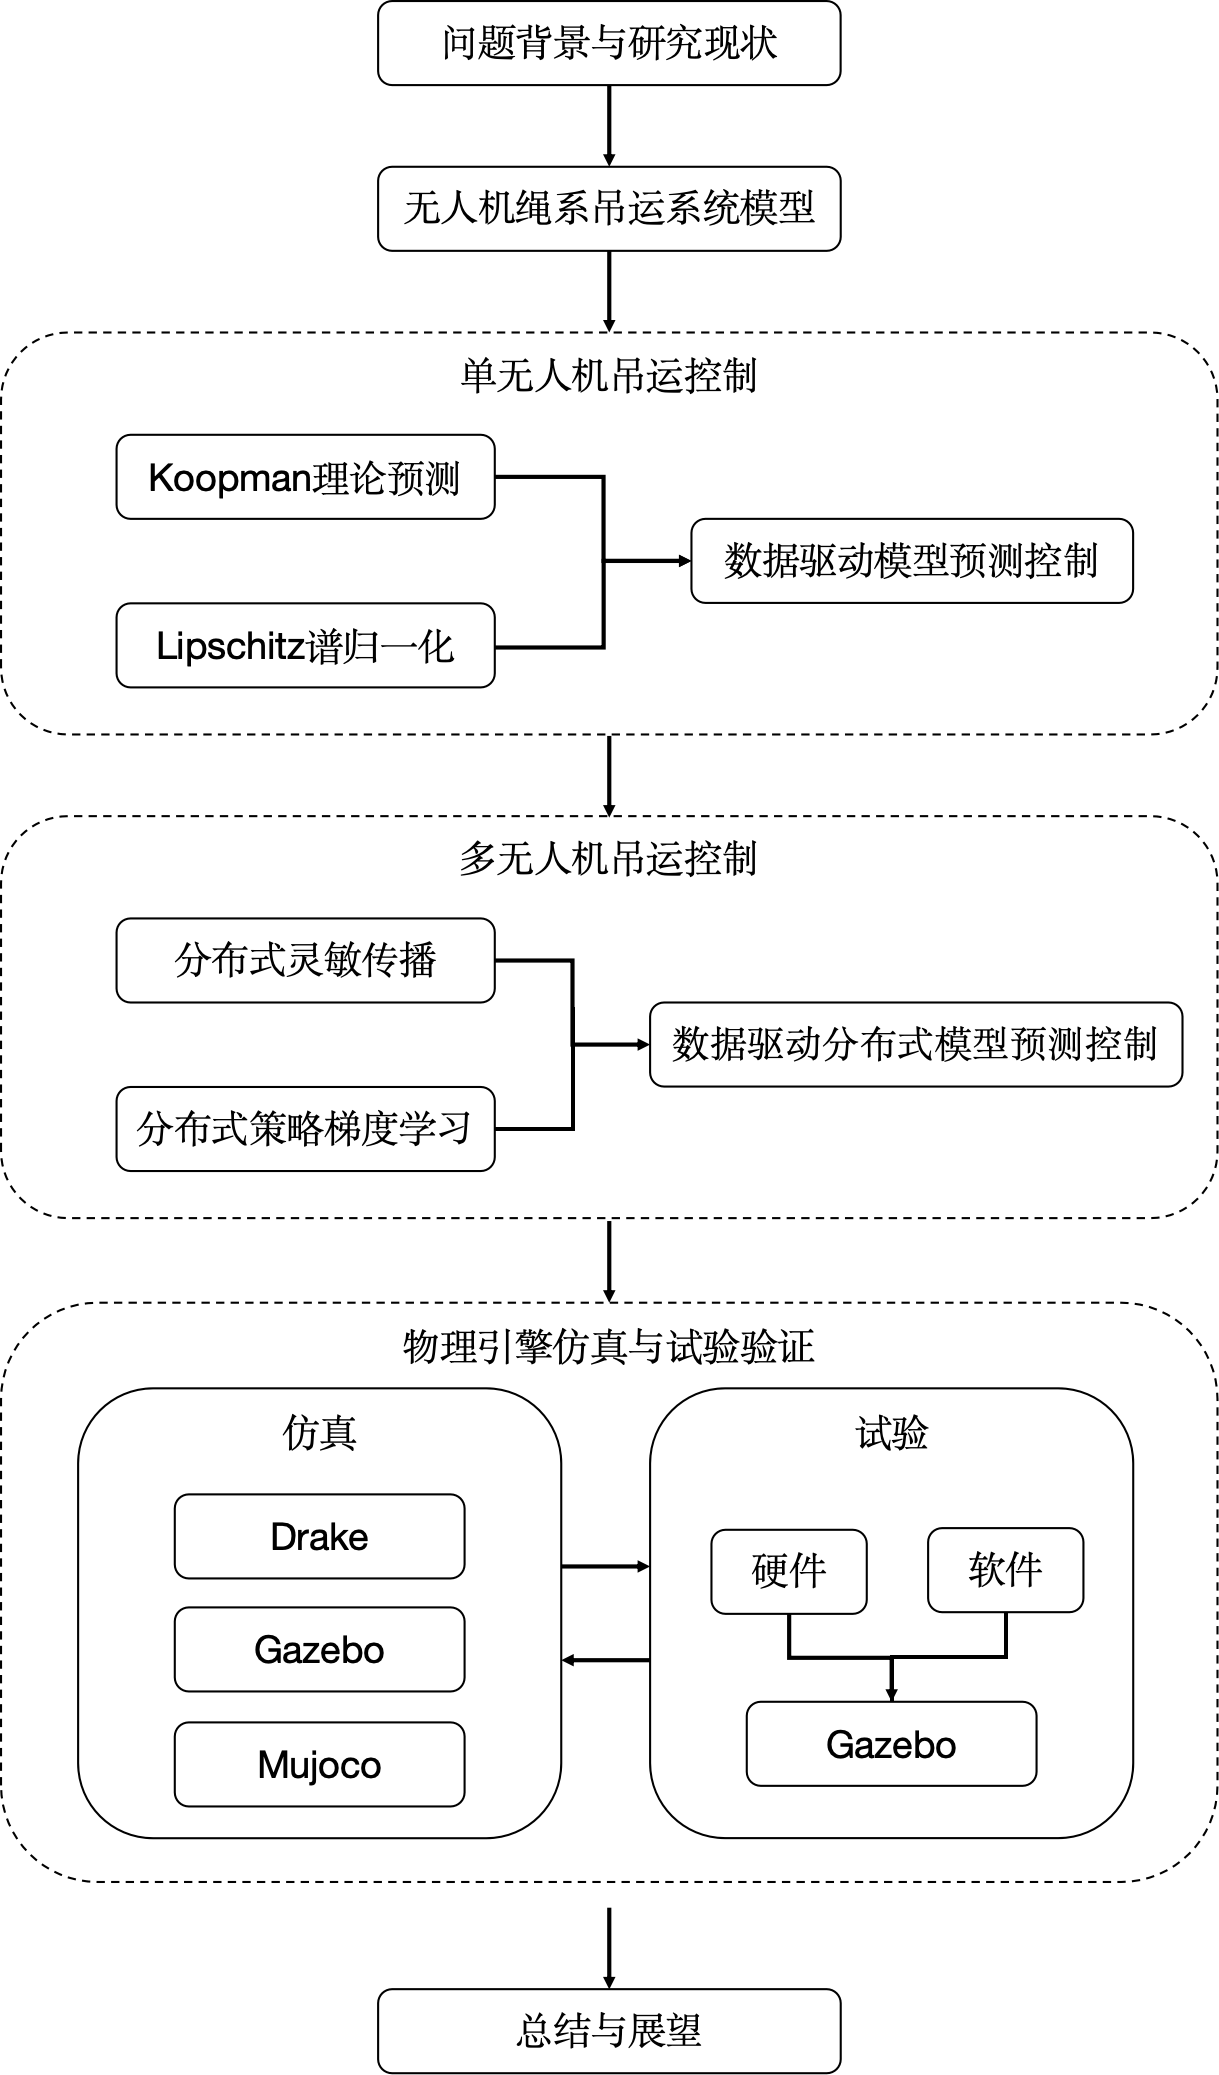
\includegraphics[width=28pc]{picture/1_0.png} 
	\caption{论文研究框架} \label{1_0}
\end{figure}

\cleardoublepage

\chapter{无人机绳系吊运系统建模}
\chaptermark{无人机绳系吊运系统建模}
在本章中,将建立无人机绳系吊运系统的动力学模型。无人机绳系吊运系统由三个子系统构成:四旋翼、系绳以及吊运的载荷,系绳和吊运的载荷会对无人机自身造成一定的扰动。本章首先对四旋翼无人机的动力学模型进行推导,然后建立单无人机绳系吊运系统的动力学方程,进而将其推广到多无人机绳系吊运系统的动力学模型中,以此作为控制模型的基础。

\section{单无人机绳系吊运系统的动力学模型}
四旋翼运输系统是一个复杂的系统,由四个旋翼组成,这些旋翼固定在刚性交叉体上。载荷通过绳系与四旋翼的主体连接,实现对载荷的精确控制和运输。
四旋翼无人机是一种基于旋翼的飞行器,由四个旋翼推动飞行。为了平衡扭矩,转子由两对对置的转子构成,一对正时针转动,一对反时针转动。四旋翼系统是高度非线性的,并且是一个欠驱动系统,有六个自由度和四个控制输入(即旋翼转速)。可以通过调整旋翼的转速来对四旋翼无人机进行控制,从而改变四旋翼无人机的扭矩和推力特性。如图\ref{2_1}所示,四旋翼无人机设计为四个旋翼交叉共振。两个相对的旋翼沿同一方向旋转,通过改变旋翼的角速度可以控制四旋翼无人机的高度和位置。如果电机$T_1$、$T_2$、$T_3$和$T_4$产生的扭矩相同,则四旋翼无人机可以保持平衡位置而不旋转。

\begin{figure}[hbt!]
	\centering
	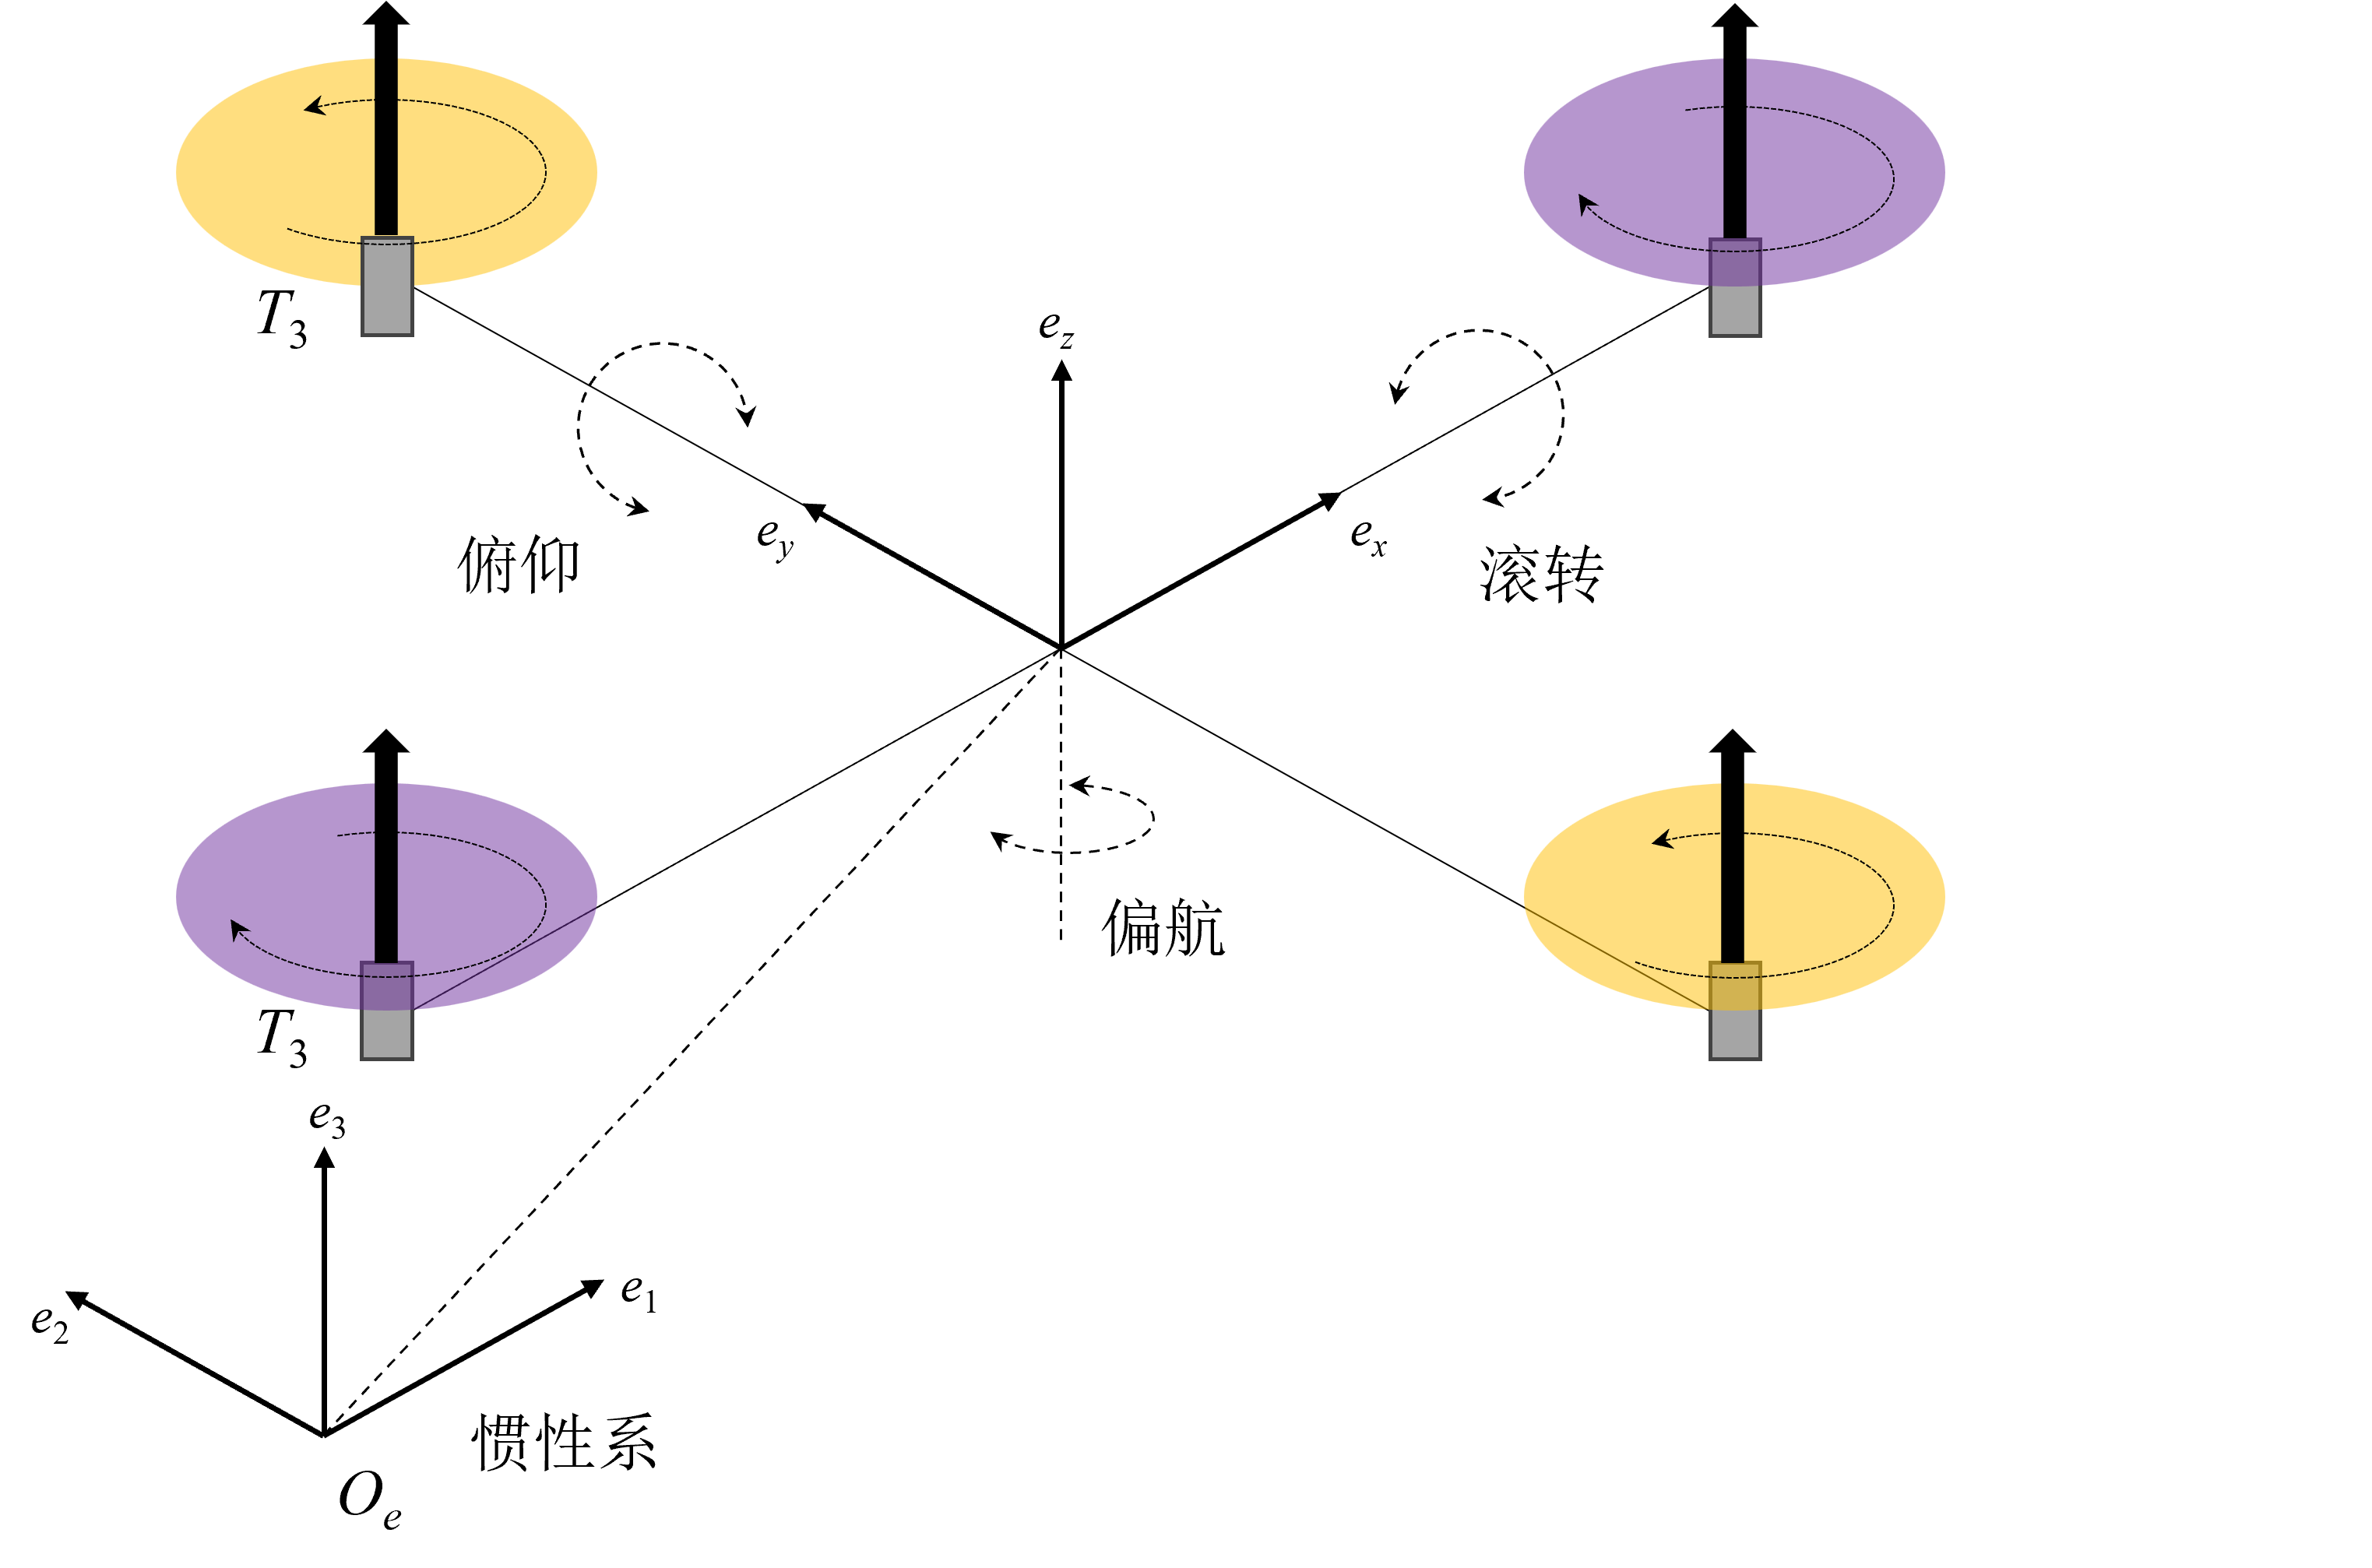
\includegraphics[width=28pc]{picture/2_1.png} 
	\caption{四旋翼无人机动力学结构} \label{2_1}
\end{figure}


对于四旋翼无人机的上升和下降,可以通过同时增加或减小电机$T_1$、$T_2$、$T_3$和$T_4$的转速来实现;滚转是四旋翼无人机通过向左或向右倾斜,以允许侧向移动的运动;俯仰是指四旋翼无人机通过前倾或后仰,向前或向后运动;偏航是指在与地面保持水平的情况下,以顺时针或逆时针的方式改变四旋翼无人机的方向。四旋翼无人机通过控制四个电机的转速,可以完成不同的飞行作业。本章根据四旋翼无人机的动力学特性建立数学模型,为下面章节控制器的设计奠定基础。


\subsection{四旋翼无人机的坐标系}
为了便于建模和描述,首先引入两个右手直角坐标系的定义,并给出两个坐标系之间的转换关系。
\subsubsection{地面坐标系}
地面坐标系$o_ex_ey_ez_e$用于研究四旋翼无人机相对于地面的运动状态,确定机体的三维位置。一般来说,在地面坐标系中,常用的局部坐标系统有 NED(North-East-Down)和ENU(East-North-Up)两种。NED坐标系$o_ex_e$轴指向正北,$o_ey_e$轴指向正东,$o_ez_e$轴垂直于地面向下。ENU坐标系 $o_ex_e$ 轴指向正东,
$o_ey_e$ 轴指向正北,$o_ez_e$ 轴垂直向上,即指向天空的方向。NED 坐标系适合飞行器或船舶等需要考虑垂直下降的系统;而ENU 坐标系更直观,符合日常地理方向的习惯,常用于地面交通、测量和定位。本文使用NED坐标系,坐标原点选择在固连于地面的任意一点。

\subsubsection{机体坐标系}
本文的四旋翼无人机为“X”型气动布局结构,运动更加灵活。
机体坐标系固连于四旋翼无人机,其原点取在四旋翼无人机的重心位置。$o_bx_b$轴在四旋翼无人机对称平面内指向机头。 $o_bz_b$轴在四旋翼无人机对称平面内,垂直轴向下。$o_by_b$轴按右手定则进行确定。机体坐标系与无人机固定连接,构成一个随四旋翼无人机运动的动坐标系。
\subsubsection{地面坐标系与机体坐标系之间的转换关系}
地面坐标系和机体坐标系的转换在无人机导航与控制中发挥着至关重要的作用。它可以帮助我们理解无人机在空间中的位置和姿态,同时实现精确的导航与控制。地面坐标系与机体坐标系之间的转换关系可以通过三个旋转矩阵来描述。具体来说,可以将地面坐标系依次沿机体坐标系进行旋转,即绕$z_b$轴旋转偏航角$\psi$,绕$y_b$旋转俯仰角$\theta$,绕$x_b$旋转滚转角$\phi$。对应的三个旋转矩阵$\boldsymbol{R}_\psi$、$\boldsymbol{R}_\theta$和$\boldsymbol{R}_\phi$分别为:
$$
\boldsymbol{R}_\psi=\begin{bmatrix}\cos\psi&-\sin\psi&0\\sin\psi&\cos\psi&0\\0&0&1\end{bmatrix} $$
$$	\boldsymbol{R}_\theta=\begin{bmatrix}\cos\theta&0&\sin\theta\\0&1&0\\-\sin\theta&0&\cos\theta\end{bmatrix} $$
$$\boldsymbol{R}_\phi=\begin{bmatrix}1&0&0\\0&\cos\phi&\sin\phi\\0&-\sin\phi&\cos\phi\end{bmatrix}
$$

因此,通过上述三个旋转矩阵,可以得到将任意矢量从地面坐标系转换到机体坐标系的转换矩阵为:
$$\begin{aligned}\boldsymbol{R}_{e-b}&=\boldsymbol{R}_{\psi}\boldsymbol{R}_{\theta}\boldsymbol{R}_{\phi}\\&=\begin{bmatrix}\cos\theta\cos\psi&\cos\theta\cos\psi&-\sin\theta\\\sin\phi\sin\theta\cos\psi-\cos\phi\sin\psi&\sin\phi\sin\theta\sin\psi+\cos\phi\cos\psi&\sin\phi\cos\theta\\\cos\phi\sin\theta\cos\psi+\sin\phi\sin\psi&\cos\phi\sin\theta\sin\psi-\sin\phi\cos\psi&\cos\phi\cos\theta\end{bmatrix}\end{aligned}$$

从机体坐标系到地面坐标系的转换矩阵为:
$$\begin{aligned}\boldsymbol{R}_{b-e}&=\bm{R}_{e-b}^\mathrm{T}\\&=\begin{bmatrix}\cos\theta\cos\psi&\sin\phi\sin\theta\cos\psi-\cos\phi\sin\psi&\cos\phi\sin\theta\cos\psi+\sin\phi\sin\psi\\\cos\theta\cos\psi&\sin\phi\sin\theta\sin\psi+\cos\phi\cos\psi&\cos\phi\sin\theta\sin\psi-\sin\phi\cos\psi\\-\sin\theta&\sin\phi\cos\theta&\cos\phi\cos\theta\end{bmatrix}\end{aligned}$$

\subsection{四旋翼无人机的模型}
四旋翼无人机模型分为运动学模型、动力学模型和控制效率模型,动力学模型既涉及运动又涉及受力情况,与物体的质量和转动惯量相关,主要用于分析无人机的受力对无人机运动速度的影响,输入为无人机旋翼产生的拉力和力矩,输出为无人机的速度和角速度。运动学模型与质量和受力无关,主要分析无人机速度对无人机位置变化产生的影响,输入为速度和角速度,输出为无人机的位置和姿态。控制效率模型输入为螺旋桨转速,输出为拉力和力矩,当已知螺旋桨转速时,可以通过控制效率模型计算出拉力和力矩。

为了简便,在对四旋翼无人机进行建模时,做了如下假设:

(1)四旋翼无人机是刚体结构,没有内力,飞行时结构无形变;

(2)四旋翼无人机的质量、螺旋桨阻力系数和转动惯量等基础参数默认不变;

(3)四旋翼无人机总保持对称结构,其几何中心与重心位置一致。



运动学方程描述了无人机位置与速度以及速度和角速度之间的关系,其运动学方程可以表示为:

\begin{equation}
    \begin{aligned}
	\dot{\boldsymbol{p}}_e &= \boldsymbol{v}_e = \bm{R}_{b-e} \bm{v}_b \\
	\bm{\Theta}_e &= \bm{W}_{b-e} * \bm{\omega}_b
\end{aligned}\label{2-1}
\end{equation}
其中,$\boldsymbol{p}_e=\left[x,y,z\right]^\mathrm{T}$为无人机在地面坐标系下的位置坐标,$\boldsymbol{v}_e=\left[v_{x},v_{y},v_{z}\right]^\mathrm{T}$为无人机在地面坐标系下的线速度,$\boldsymbol{v}_b=\left[u,v,w\right]^\mathrm{T}$表示无人机在机体坐标系下的线速度,$u$、$v$、$w$表示分别沿$x$、
$y$、$z$机体坐标轴方向的线速度分量,$\boldsymbol{R}_{b-e}$为上一小节定义的转换矩阵,$\bm{\Theta}_e=\left[\phi,\theta,\psi\right]^\mathrm{T}$表示无人机在地面坐标系下的姿态角度,$\bm{W}_{b-e}$表示地面坐标系下欧拉角速度变换到机体旋转角速度的旋转矩阵,$\boldsymbol{\omega}_b=\left[{\omega}_{xb},{\omega}_{yb},{\omega}_{zb}\right]^\mathrm{T}$ 为无人机机体坐标系下的角速度,可以得到姿态旋转矩阵具体形式如式(\ref{2-2})所示:
\begin{equation}
	\boldsymbol{\omega}_b=\begin{bmatrix}\omega_{xb}\\\omega_{yb}\\\omega_{zb}\end{bmatrix}=\begin{bmatrix}1&0&-\sin\theta\\0&\cos\phi&\cos\theta\sin\phi\\0&-\sin\phi&\cos\theta\cos\phi\end{bmatrix}\begin{bmatrix}\dot\phi\\\dot\theta\\\dot\psi\end{bmatrix}
	\label{2-2}
\end{equation}



一般来说,四旋翼无人机飞行时其姿态角在小范围内运动,可以近似认为有下式成立:
\begin{equation}
	\boldsymbol{\omega}_b=\begin{bmatrix}{\omega}_x\\{\omega}_y\\{\omega}_z\end{bmatrix}=\begin{bmatrix}\dot{\phi}\\\dot{\theta}\\\dot{\psi}\end{bmatrix}
	\label{2-3}
\end{equation}

以上详细描述了四旋翼无人机系统的运动学模型以及其在不同坐标系下的位置与线速度、角度与角速度之间的转换关系。接下来,将无人机整体视为一个刚体,将其分解为平移运动和旋转运动两个部分。通过牛顿法分析其平移运动,通过欧拉法分析其旋转运动,从而构建其动力学模型。其动力学的基本方程如式(\ref{2-4})所示:
\begin{equation}
	\begin{aligned}
		m\dot{\boldsymbol{v}}_e&=mg\bm{e}_{3}-\boldsymbol{R}_{b-e}f\bm{e}_{3}\\
		\boldsymbol{J}\dot{\boldsymbol{\omega}_b}&=-\bm \omega_b \times \bm J \bm \omega_b+\boldsymbol{\tau}
	\end{aligned}\label{2-4}
\end{equation}
其中$m$为无人机的质量,$g\in\mathbb{R}_+$为重力加速度,$\bm{e_{3}}=\left[0,0,1\right]^\mathrm{T}$,$\boldsymbol{\tau}=\left[\tau_x,\tau_y,\tau_z\right]^\mathrm{T}$表示无人机四个螺旋桨产生的扭矩,$\boldsymbol{J}$为无人机的惯量矩阵,$f\in\mathbb{R}_+\cup\{0\}$表示无人机螺旋桨总拉力的大小,该拉力是单向的,其形式如式 (\ref{2-5})所示:
\begin{equation}
	f=\sum_{i=1}^4f_i=c_\mathrm{T}\Omega_i^2
	\label{2-5}
\end{equation}
其中$f_i$表示表示一个旋翼在机体坐标系下旋转产生的升力,与旋翼的转速的平方正相关。$c_\mathrm{T}=1/4\pi^2\cdot\rho D_\mathrm{p}^4C_\mathrm{T}$为螺旋桨的升力系数,其大小与无人机自身的材质、倾斜角等因素有关,$\Omega_i$为
单个螺旋浆的旋转速度。由于本文采用“X”型气动布局,实际力臂长度是机臂长度的$\sqrt{2}/2$倍,可以得到无人机每个螺旋桨产生的力矩如式(\ref{2-6})所示:


\begin{equation}
	\left\{ \begin{array}{l}
		\tau_x={\sqrt{2}}/{2}dc_\mathrm{T}\left(\Omega_1-\Omega_2-\Omega_3+\Omega_4\right)\\
		\tau_y={\sqrt{2}}/{2}dc_\mathrm{T}\left(\Omega_1+\Omega_2-\Omega_3-\Omega_4\right)\\
		\tau_z=c_\mathrm{M}\left(\Omega_1-\Omega_2+\Omega_3-\Omega_4\right)\\
	\end{array} \right.
		\label{2-6}
\end{equation}
其中$c_M$为螺旋桨的反扭力系数,其产生的力矩方向沿$z$轴方向。$d\in\mathbb{R}_+$为无人机重心和任一电机转动轴线之间的距离。为了能够对应控制器中的控制量,定义虚拟控制变量为$\bm{U}=\left[U_1,U_2,U_3,U_4\right]^\mathrm{T}=\left[f,\tau_x,\tau_y,\tau_z\right]^\mathrm{T}$,那么,将式(\ref{2-2})、(\ref{2-3})、(\ref{2-5})、(\ref{2-6})代入式(\ref{2-1})和(\ref{2-4})中,即可得到四旋翼无人机的控制模型:


\begin{equation}
		\left\{
	\begin{aligned}
		&\dot{x}=v_{x}\\
		&\dot{y}=v_{y}\\
		&\dot{z}=v_{z}\\
		&\ddot{x}=\frac{U_{1}}{m}\left(\cos\phi\cos\psi\sin\theta+\sin\phi\sin\psi\right)\\
		&\ddot{y}=\frac{U_{1}}{m}\left(\cos\phi\sin\psi\sin\theta-\cos\psi\sin\phi\right)\\
		&\ddot{z}=\frac{U_{1}}{m}\left(\cos\phi\cos\theta\right)-g\\
		&\dot{\phi}={\omega}_x+\tan\theta\left({\omega}_y\sin\phi+{\omega}_z\cos\phi\right)\\
		&\dot{\theta}={\omega}_y\cos\phi-{\omega}_z\sin\phi\\
		&\dot{\psi}=\frac{{\omega}_y\sin\phi+{\omega}_z\cos\phi}{\cos\theta}\\
		&\ddot{\phi}=\frac{(I_{y}-I_{z})\cdot \dot{\theta}\dot{\psi}+U_{2}}{I_{x}}\\
		&\ddot{\theta}=\frac{(I_{z}-I_{x})\cdot \dot{\phi}\dot{\psi}+U_{3}}{I_{y}}\\
		&\ddot{\psi}=\frac{(I_{x}-I_{y})\cdot \dot{\phi}\dot{\theta}+U_{4}}{I_{z}}\end{aligned}
	\right.
	\label{2-7}
\end{equation}
\subsection{四旋翼无人机绳系吊运系统的动力学模型}
在本文的吊装运输场景中,四旋翼无人机在满足自身飞行需求的同时,还会受到吊装载荷对其作用的拉力干扰,单无人机吊装载荷受力分析如图 \ref{2_2} 所示,其中$F$表示无人机的升力,$G$表示无人机自身的重力,$G_0$表示无人机自身的重力,$T$表示载荷对无人机产生的拉力,$\theta$表示系绳与垂直平面之间的夹角。
\begin{figure}[hbt!]
	\centering
	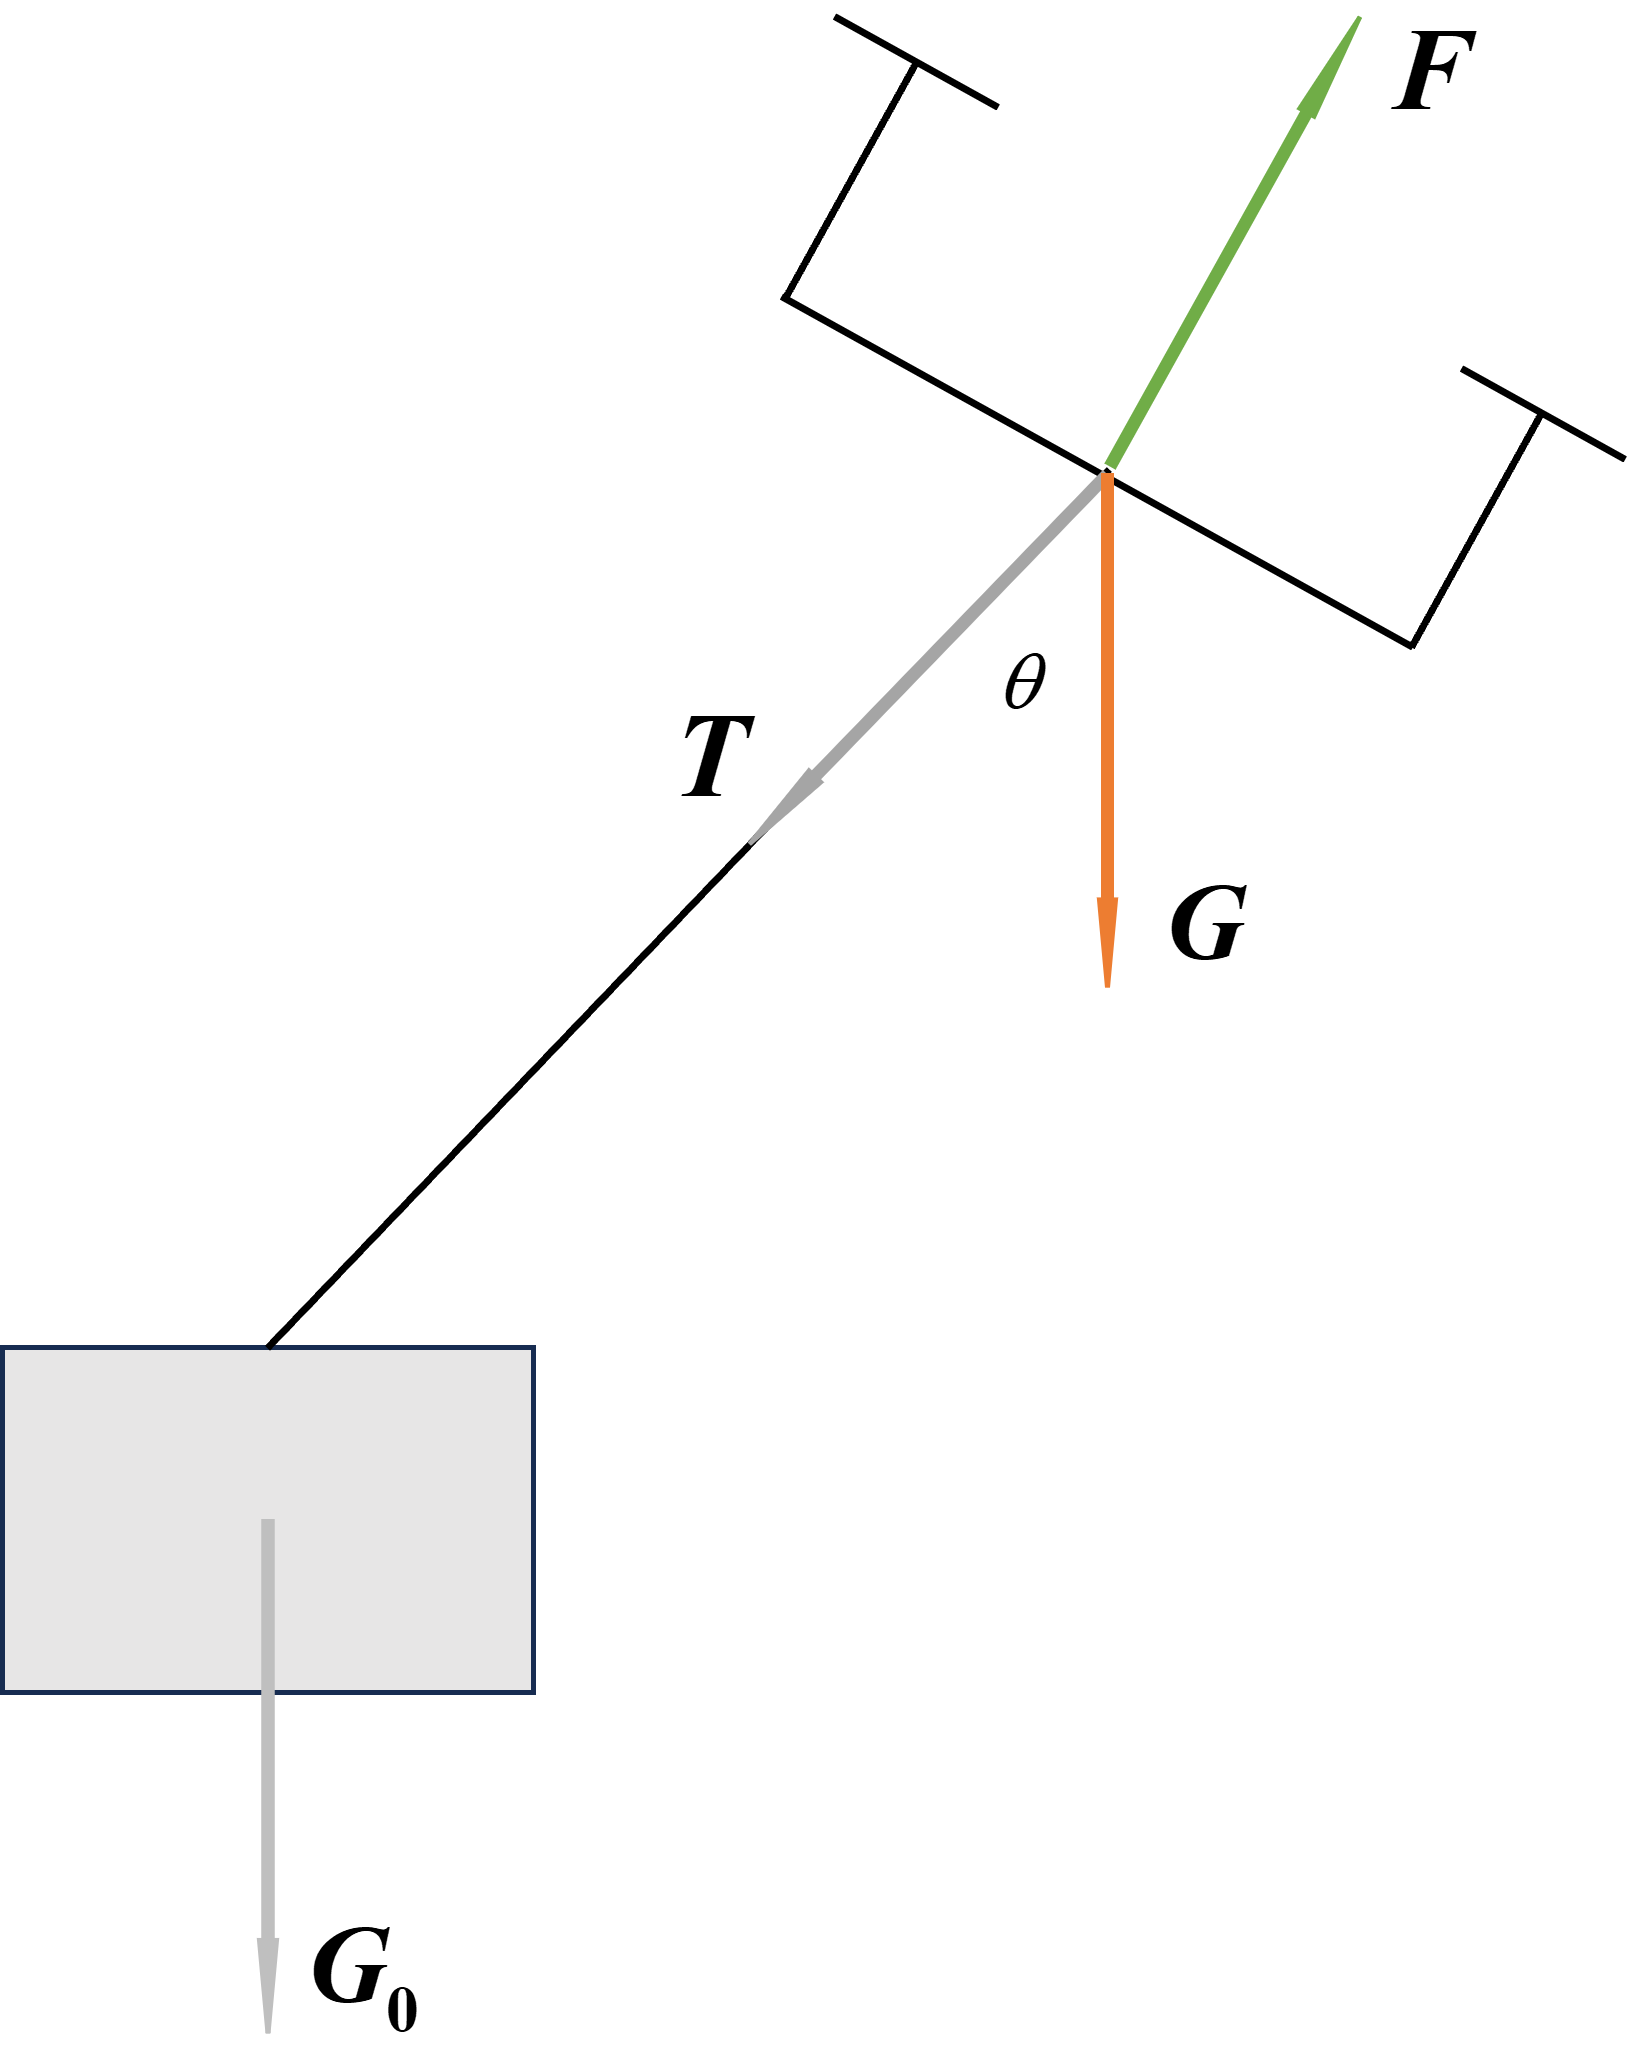
\includegraphics[width=21pc]{picture/2_2.png} 
	\caption{单无人机吊装载荷受力分析} \label{2_2}
\end{figure}

对于四旋翼无人机绳系吊运系统来说,在轨迹跟踪时其系绳并不一定总是保持绷直状态的,在无人机的高速移动中系绳上的张力可能为零。因此,本文建立四旋翼无人机绳系吊运系统的混合模型,考虑系绳上的张力不为零和张力为零这两种情况。

\subsubsection{系绳张力不为零时的动力学模型}

四旋翼无人机绳系吊运系统由载荷相对于地面坐标系的位置、载荷姿态和四旋翼无人机的姿态来定义。当系绳拉紧时,该系统具有八个自由度,并存在四个自由度的欠驱动。四旋翼无人机和载荷的位置之间的关系为:

\begin{equation}
	\bm p_q\bm p_l-l\bm q
\end{equation}
其中$\bm p_q$、$\bm p_l$分别为四旋翼无人机和载荷的位置,$l$为系绳的长度,$\bm q$表示从四旋翼无人机质心指向载荷质心的单位向量。本文采用拉格朗日法来推导运动方程。系统的拉氏量 $\mathcal{L}:T\bar{Q}\to\mathbb{R}$ 定义为$\mathcal{L}=\mathcal{T}-\mathcal{U}$,其中$\mathcal{T}:TQ\to\mathbb{R}$和${\mathcal{U}}:Q\to\mathbb{R}$分别是机械系统的动能和势能,它们的定义如下:

\begin{equation}
\begin{aligned}
	\mathcal{T}=\frac{1}{2}&m_{q}\bm v_{q}\cdot \bm v_{q}+\frac{1}{2}m_{l}\bm v_{l}\cdot \bm v_{l}+\frac{1}{2}\langle\hat{\bm  \omega_q},\widehat{\bm J_{q}\bm  \omega_q}\rangle\\
	&\mathcal{U}=m_{q}g\bm e_{3}\cdot \bm x_{Q}+m_{l}g\bm e_{3}\cdot \bm x_{l}
\end{aligned}
	\label{2-9}
\end{equation}
其中$\bm v_q$、$\bm v_l$分别为无人机和载荷的速度,$m_q$、$m_l$分别为无人机和载荷的质量,$\langle\cdot,\cdot\rangle $表示内积,$\hat{.}$被定义为使得 $\hat{\bm x}\bm y=\bm x\times \bm y$对于所有$\bm x,\bm y\in\mathbb{R}^3$恒成立,$\omega_q$为四旋翼无人机在机体坐标系下的角速度。在本文中,$\lambda_m(\cdot)$和 $\lambda_n(\cdot)$ 分别表示矩阵的最小和最大特征值。系统的动力学满足拉格朗日原理:
\begin{equation}
	\bm \delta\int_0^\tau\mathcal{L} dt+\int_0^\tau\left(\langle \bm W_1,\hat{\bm \tau}\rangle+\bm W_2\cdot f\bm{R}_{b-e}\bm e_3\right) dt=0
	\label{2-10}
\end{equation}
其中$\bm W_{1}=\bm R_{b-e}^\mathrm{T}\bm \delta \bm R_{b-e}$是定义在旋转空间上的变分向量场, $ \bm W_{2}=\bm \delta \bm x_{Q}=\bm \delta \bm x_{L}-l\bm \delta q$是定义在平移空间上的变分向量场,两者共同描述刚体系统中的变分动态,并且满足以下条件:
\begin{equation}
	\begin{aligned}
	&\bm \delta \bm q = \bm \xi \times \bm q\\
	\bm \delta \dot{\bm q} = &\dot{\bm \xi} \times \bm q + \bm \xi \times \dot{\bm q} \\
	\bm \delta\bm  R&_{b-e} = \bm R_{b-e} \hat{\bm \eta} \\
	\bm \delta \hat{\bm  \omega _q}& = \widehat{\hat{\bm  \omega_q} \bm \eta} + \hat{\dot{\bm \eta}}
\end{aligned}
\end{equation}
其中$\bm \delta \bm q$为二维球面上的变分,$\bm \delta \bm R$为三维空间上的变分。
向量 $\bm{\xi} \in \mathbb{R}^3$ 是一个三维实数向量,满足 $\bm{\xi}$ 与向量 $\bm{q}$ 的点积为零,即$\bm{\xi}$ 垂直于 $\bm{q}$,向量 $\bm{\eta} \in \mathbb{R}^3$ 是一个三维实数向量。

由于(\ref{2-10})对所有可能的变化都是满足的,因此得到带有系绳载荷的四旋翼无人机的运动方程为:

\begin{equation}
	\begin{aligned}
		&\dot{\bm x}_{l}=\bm v_{l} \\
		(m_q+m_l)(\dot{\bm v}_L+g\bm e_3)& =(\bm q\cdot f\bm R\bm e_3-m_Ql(\dot{\bm q}\cdot\dot{\bm q}))\bm q \\
		&\dot{\bm q}=\bm \omega_l\times \bm q \\
		m_{q}l \dot{\bm \omega_l}&=-\bm q\times f\bm R\bm e_{3} \\
		&\dot{\bm R_{b-e}}=\bm R_{b-e}\hat{\bm  \omega_q} \\
		\bm J_{q}\dot{\bm  \omega_q}+&\bm  \omega_q\times \bm J_{q}\bm  \omega_q=\bm \tau
	\end{aligned}
\end{equation}

上述动力学可以写成标准形式 $\dot{\bm X}_n=\bm f_n(\bm X_n)+\bm g_n(\bm X_n)\bm u$ ,其中 $\bm X_n = \{\bm x_l,\bm q,\bm R_{b-e},\bm v_l,\bm \omega_l,\bm \omega_q\}$ 是系统的状态,$\bm u = \left[f,\bm \tau \right]$是系统的输入。
\subsubsection{系绳张力为零时的动力学模型}
当系绳张力趋于零时,四旋翼无人机和吊挂载荷作为独立系统,载荷处于自由落体状态。在这种情况下,四旋翼无人机绳系吊运系统的运动方程为:
\begin{equation}
	\begin{aligned}
	&\dot{\bm x}_{l}=\bm v_{l}\\
	\quad m_{l}(&\dot{\bm v}_{l}+g\bm e_{3})=0\\
	&\dot{\bm x}_{q}=\bm v_{q}\\
	\quad m_{q}(\dot{\bm v}_{q}&+g\bm e_{3})=f\bm R_{b-e}\bm e_{3}\\
	&\dot{\bm R_{b-e}}=\bm R_{b-e}\hat{\Omega}\\
	\quad \bm J_{q}\dot{\bm \Omega}+&\bm \Omega\times \bm J_{q}\bm \Omega=\bm \tau
\end{aligned}
\end{equation}
上述方程也可以写成标准形式$\dot{\bm X}_z=\bm f_z(\bm X_z)+\bm g_z(\bm X_z)\bm u$,其中中$\bm X_z = \{\bm x_L,\bm x_q,\bm R_{b-e},\bm v_l,\bm v_q,\bm \omega_b\}$为状态。

\subsubsection{混合系统的动力学模型}
系绳悬挂载荷的四旋翼无人机是一个混合系统,因为当缆索中的张力降为零或当张力恢复时松弛的缆索变得绷紧时,动力学会发生切换。混合模型可以写成,
\begin{equation}
	\left.\begin{aligned}&\Sigma_{n}:\left\{\begin{array}{ll}\dot{\bm X_n}=\bm f_n(\bm X_n)+\bm g_n(\bm X_n)\bm u  &\bm X_n\notin \mathbb{S}_z\\\bm X_z^+=\Delta_{n\to z}(\bm X_n^-)  &\bm X_n\in \mathbb{S}_z\end{array}\right.\\&\Sigma_{z}:\left\{\begin{array}{ll}\dot{\bm X_z}=\bm f_z(\bm X_z)+\bm g_z(\bm X_z)\bm u \ \ &\bm X_z\notin \mathbb{S}_n\\\bm X_n^+=\Delta_{z\to n}(\bm X_z^-) \ &\bm X_z\in \mathbb{S}_n\end{array}\right.\end{aligned}\right.
\end{equation}
其中集合$\mathbb S_z = \{ \bm X_n \mid  T \equiv 0 \}$,$\mathbb S_n = \{ \bm X_z \mid \|\bm x_Q - \bm x_L\| \equiv l, d \|\bm x_Q - \bm x_L\| /dt> 0 \}$,系绳上的张力定义为$T = \|m_L (\ddot{\bm x}_L + g\bm{e}_3)\|$,状态转移映射$\Delta_{n\to z}$为单位映射,$\Delta_{z\to n}$为两个物体非弹性碰撞的模拟,并满足条件$\dot{\bm x}_Q^+-\dot{\bm x}_L^+=0$。

\section{多无人机绳系吊运系统的动力学模型}
由于单个无人机的承载能力有限,提出了多无人机协同吊装运输方案,显著提升系统的承载能力。当无人机数量$n\geq3$时,多架无人机可以协同对载荷进行精准控制。本文研究由三架规格型号相同的四旋翼无人机协同运输吊挂载荷的问题。该吊运系统
由三个四旋翼无人机、三根系绳和需要被运输的载荷组成。三个四旋翼无人机协同吊装运输载荷的飞行系统示意图如图 \ref{2_3} 所示,每个四旋翼无人机用
$q1$,$q2$,$q3$ 表示,吊挂载荷用$p$表示,三架无人机保持水平高度一致,无人机之间的相对距离为$d$。

\begin{figure}[hbt!]
	\centering
	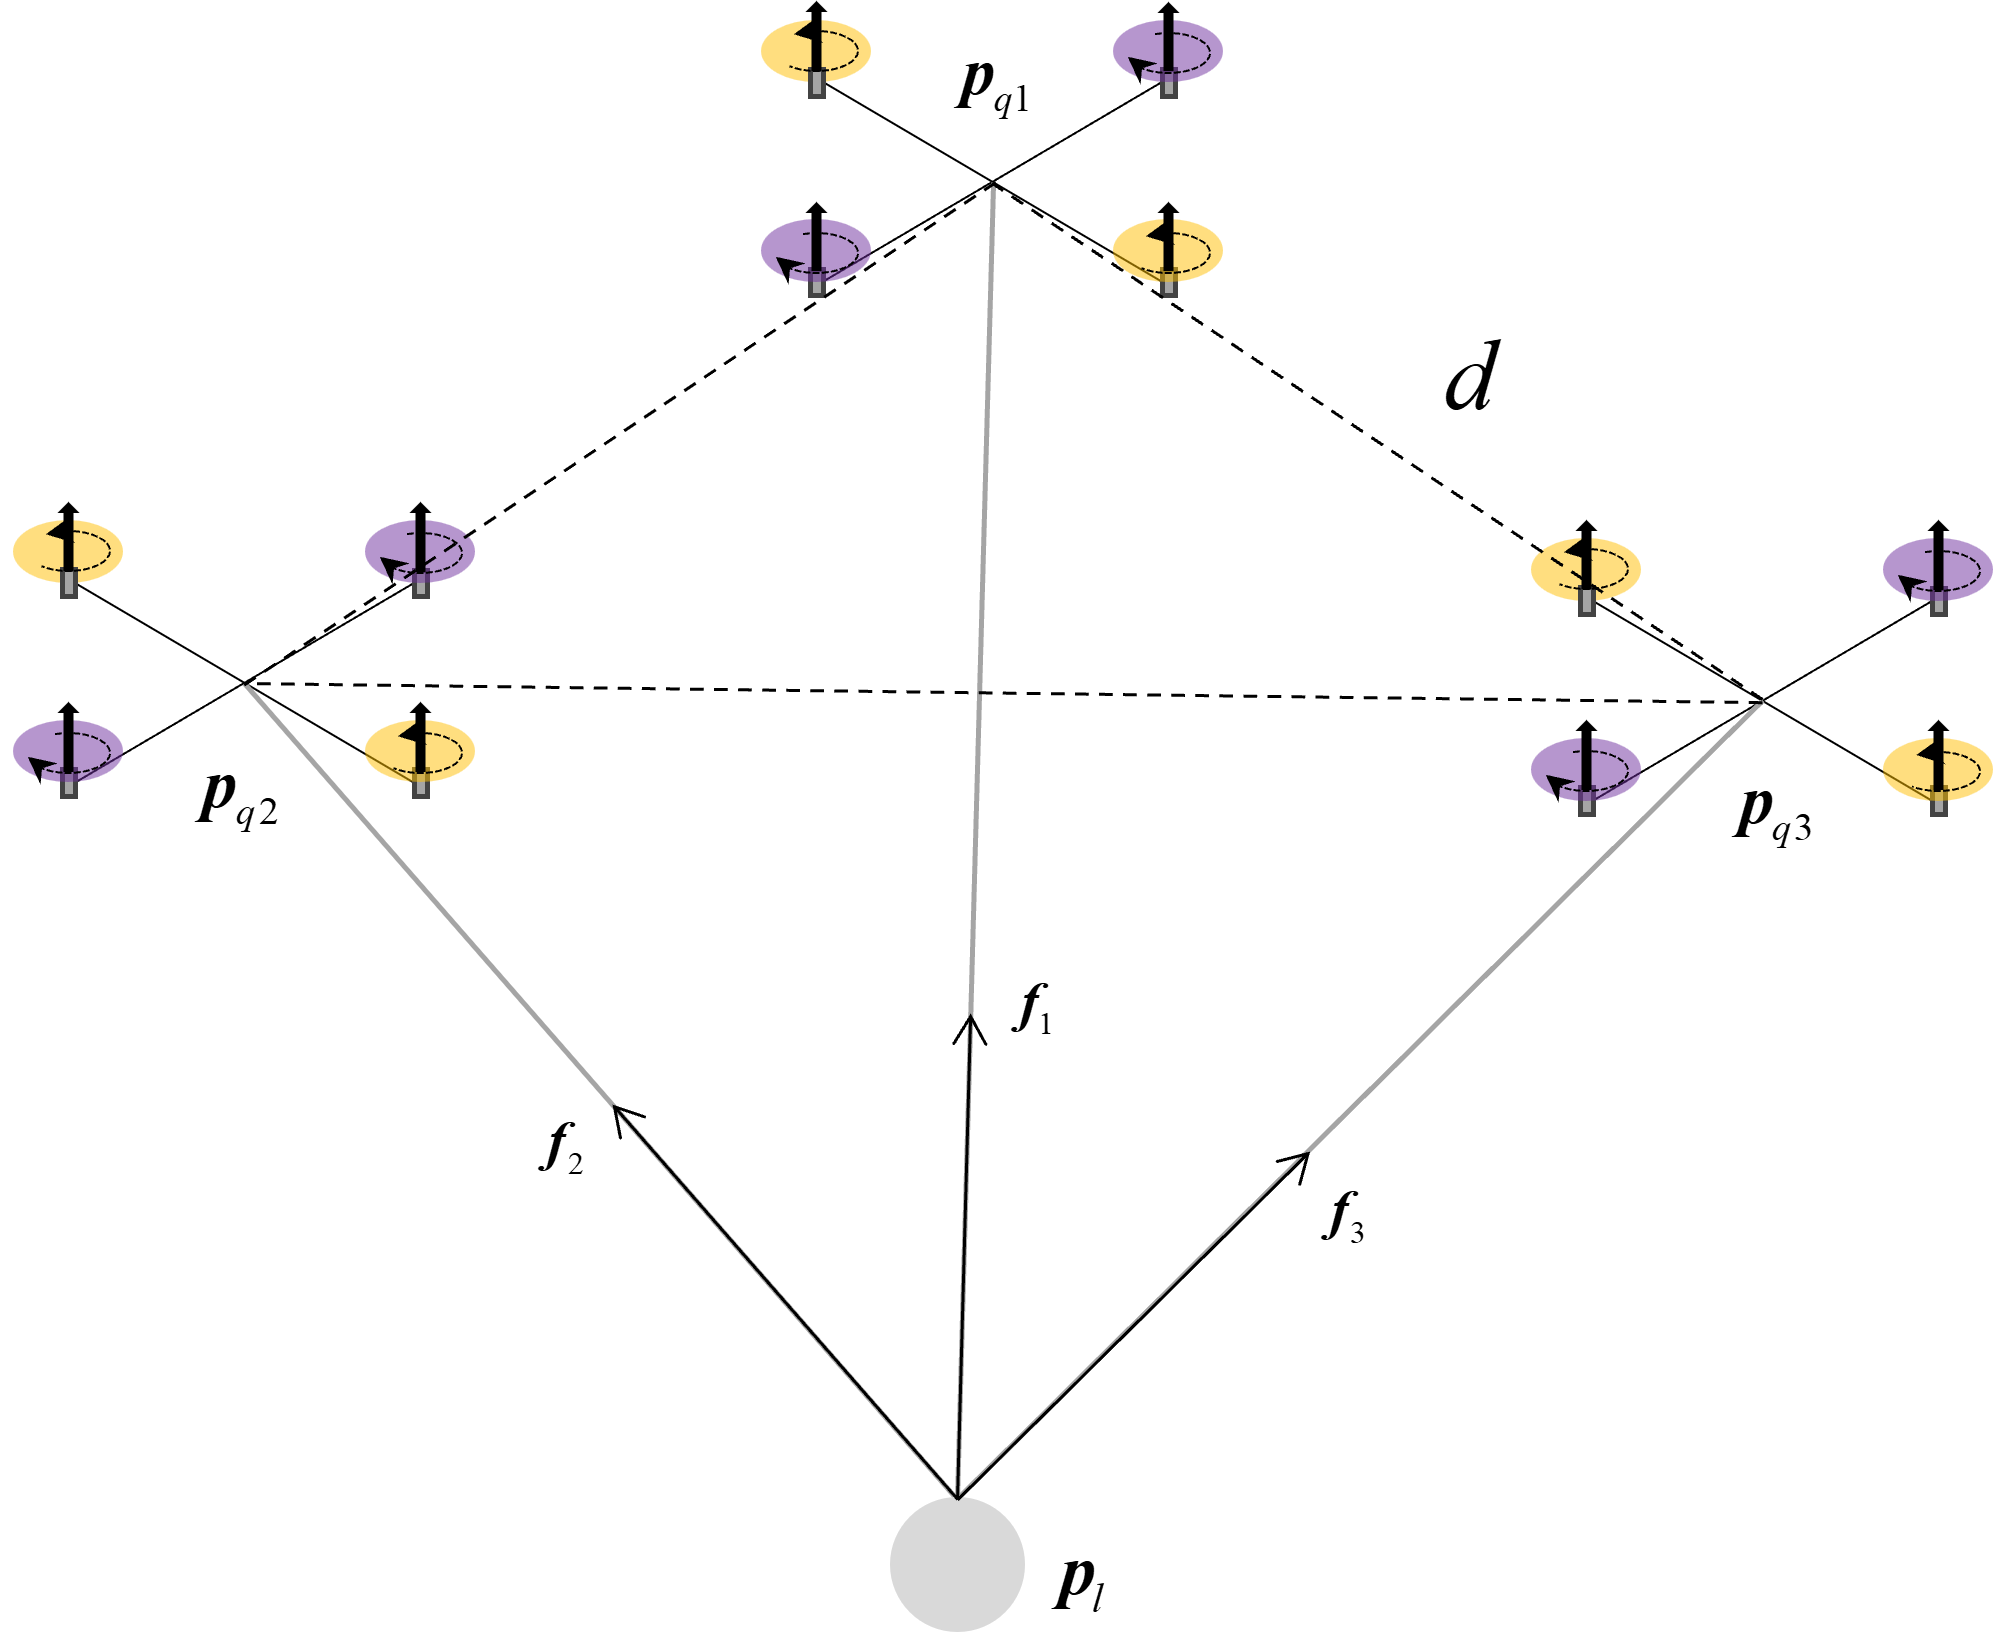
\includegraphics[width=28pc]{picture/2_3.png} 
	\caption{多无人机吊运系统} \label{2_3}
\end{figure}

在推导多无人机绳系吊运系统的动力学模型之前,先做了如下假设:



(1)无人机绳系吊运系统所吊挂的载荷被视为刚体; 


(2)连接无人机与有效载荷之间的系绳没有质量,且不会发生缠绕;

(3)所有系绳都连接在无人机的质心处,系绳的牵引力能够影响无人机的平
动,但是不影响无人机的转动。 

基于上述假设,本小节将建立多无人机绳系吊运系统的动力学模型。


在地面坐标系下,载荷位置向量为$p_{l}=[p_{lx},p_{ly},p_{lz}]^{\mathrm{T}}$,三个无人机的位置向
量分别用$p_{q1}$、$p_{q2}$、$p_{q3}$来表示,吊绳长度为$L$。对悬吊的载荷进行受力分析,由牛顿第二定律可得出:
\begin{equation}
	\label{2-15}
	\begin{aligned}
		&f_{Li}=\frac{1}{L}(p_{qi}-p_{l})T_{i} \\
		&m_{1}\ddot{p}_{1}=-m_{1}ge_{3}+\sum_{i=1}^{3}f_{Li}
	\end{aligned}
\end{equation}
其中$f_{Li}$表示第i根绳子在惯性坐标系下所提供的拉力向量;$T_{i}$表示第$i$根绳子提供的拉力值标量。

对于系统来说,$\alpha_{i}$和$\beta_i$分别描述了系绳在地面坐标系 下相对于吊挂载荷的偏角,从载荷
质心到无人机质心的单位方向向量为:
\begin{equation}
	\boldsymbol{q}_i=\left[\cos\alpha_i\cos\beta_i,\sin\alpha_i\cos\beta_i\,\sin\beta_i\right]^\mathrm T
\end{equation}

默认在实际过程中吊挂载荷始终位于三架四旋翼无人机之间,$\alpha_{i}$和$\beta_i$满足条件:
$0^\circ\leq\alpha_i\leq360^\circ$,$0^\circ\leq\beta_i\leq90^\circ$,再考虑到各个无人机在飞行中可能碰撞的情况,实际的$\beta_i$应该处在一个更小的合理范围内。

类似(2-5),确定吊挂载荷的位置后,可以确定三架无人机的位置:
\begin{equation}
\begin{aligned}
	\boldsymbol{p}_{l}=&\left[p_{l_{x}},p_{l_{y}},p_{l_{z}}\right]^{\mathrm{T}} \\
	\boldsymbol{p}_{q1}&=\boldsymbol{p}_l+l\boldsymbol{q}_1 \\
	\boldsymbol{p}_{q2}&=\boldsymbol{p}_{l}+l\boldsymbol{q}_{2} \\
	\boldsymbol{p}_{q3}&=\boldsymbol{p}_l+l\boldsymbol{q}_3
\end{aligned}
\end{equation}
上式中,$\bm{p}_{q1}$,$\bm{p}_{q2}$,$\bm{p}_{q3}$和$\bm{p}_l$分别表示三个无人机和吊挂载荷的位置,$l$是系
绳长度。

与前文类似,无人机的控制输入为$\bm{U}=\left[U_1,U_2,U_3,U_4\right]^\mathrm{T}=\left[f_i,\tau_{x_i},\tau_{y_i},\tau_{z_i}\right]^\mathrm{T}$,其中$f_{i}$,$\tau_{x_i}$,$\tau_{y_i}$,$\tau_{z_i}$表示第 $i$ 个无人机的控制力和控制力矩大小,具体表述参
考式(\ref{2-5})和(\ref{2-6})。
同时,为了模拟系统受到的未知扰动(四旋翼无人机的诱导气流等),考虑有一个直接作用在吊挂载荷上的外界干扰力${\boldsymbol{f}}_{w}=\left[F_{xw},F_{yw},F_{zw}\right]^\mathrm{T}$。

在三个四旋翼无人机绳系吊挂载荷系统中,存在三个非零张力系绳产生的完整约束,不考虑载荷的刚体转动情况下,整个系统自由度为18(6×3+3-3)。本文为方便后续多机吊挂研究,选择吊挂载荷的位置,三个无人机的姿态角以及三根系绳与吊挂载荷形成的偏离角度作为系统的广义坐标,记作:
$$\boldsymbol{X}_n=
\left[
	p_{l_x} , p_{l_y} , p_{l_z},\alpha_1,\beta_1,\phi_1,\theta_1,\psi_1,\alpha_2,\beta_2,\phi_2,\theta_2,\psi_2,\alpha_3,\beta_3,\phi_3,\theta_3,\psi_3
\right]^\mathrm T$$

类似式(\ref{2-9}),三个无人机吊挂载荷系统的动能和势能可分别表示如下:
\begin{equation}
	\begin{aligned}
	\mathcal{T}=\frac{1}{2}m_{l}{\boldsymbol{v}}_{l}^\mathrm{T}{\boldsymbol{v}}_{l}+&\frac{1}{2}\left[\sum_{i=1}^{3}\left(m_{q_{i}}\dot{\boldsymbol{v}}_{q_{i}}^{T}\dot{\boldsymbol{v}}_{q_{i}}+\boldsymbol{\omega}_{q_{i}}^{T}\boldsymbol{J}_{q_{i}}\boldsymbol{\omega}_{q_{i}}\right)\right] \\
	\mathcal{U}=\sum_{i=1}^{3}&m_{q_{i}}g\boldsymbol{e}_3\cdot\boldsymbol{x}_{q_{i}}+m_{l}g\boldsymbol{e}_3\cdot\boldsymbol{x}_{l}
\end{aligned}
\label{2-18}
\end{equation}
其中,$m_{q_{i}}$,$m_l$ 表示第 $i$ 个无人机和吊挂载荷的质量,

$\boldsymbol{J}_{q_{i}}$ 为无人机的转动惯量。
可以得到系统的欧拉-朗格朗日方程为:
\begin{equation}
\begin{aligned}
	&\mathcal{L}=\mathcal{T}-\mathcal{U} \\
	\boldsymbol{F}_{\boldsymbol{X}_n}=&\frac{\mathrm{d}}{\mathrm{d}t}\left(\frac{\partial\mathcal{L}}{\partial\dot{\boldsymbol{X}_n}}\right)-\frac{\partial\mathcal{L}}{\partial\boldsymbol{X}_n}
\end{aligned}
\label{2-19}
\end{equation}


把式(\ref{2-18})代入式(\ref{2-19})中可得到如下二阶非线性微分方程:
\begin{equation}	
	\dot{\bm X}_n=\bm f_n(\bm X_n)+\bm g_n(\bm X_n)\bm u+\bm k_{n}\left(\bm f_{w}\right)
\end{equation}
其中$\bm k_{z}\left(\bm F_{p}\right)$为未知的外部干扰。
进一步选择状态向量为:$$\bm X=\left[x_{p},x_{p},y_{p},y_{p},z_{p},z_{p},\alpha_{i},\dot{\alpha}_{i},\beta_{i},\dot{\beta}_{i},\phi_{i},\dot{\phi}_{i},\theta_{i},\dot{\theta}_{i},\psi_{i},\dot{\psi}_{i}\right]^\mathrm{T}$$
记$\bm{U}=\left[f_i,\tau_{x_i},\tau_{y_i},\tau_{z_i}\right]^\mathrm{T}$作为控制力、力矩向量,${\boldsymbol{U}}_{w}=\left[F_{xw},F_{yw},F_{zw}\right]^\mathrm{T}$为外部干扰输入,从而把式(2-24)转换为一阶非线性微分方程:
\begin{equation}
	\dot{\boldsymbol{X}}=\bm f\left(\boldsymbol{X},\boldsymbol{U}\right)+\bm f_w\left(\boldsymbol{U}_w\right)
	\label{2-21}
\end{equation}

式(\ref{2-21})可以完整地描述出三个四旋翼无人机运输吊挂载荷的动力学模型,而且当无
人机数量增加时,只需在状态变量中相应增加系绳偏角α、β即可。但是在实际运输控制中,无人机的控制器很难获取系绳偏角和吊挂载荷的位置信息,依照现有模型无法进
行控制器设计,因
此需要一个不包含载荷信息的简化模型,可以将系绳拉力可以被当作对无人机平动运动
的一个干扰力,绳子牵引力作用下的第$i$架无人机动力学模型为: 
\begin{equation}
	\left\{
	\begin{aligned}
		&\ddot{x}=\frac{U_{1i}\left(\cos\phi_i\cos\psi_i\sin\theta_i+\sin\phi_i\sin\psi_i\right)-f_{xi}}{m}+d_{xi}\\
		&\ddot{y}=\frac{U_{1i}\left(\cos\phi_i\sin\psi_i\sin\theta_i-\cos\psi_i\sin\phi_i\right)-f_{yi}}{m}+d_{yi}\\
		&\ddot{z}=\frac{U_{1i}\cos\phi_i\cos\theta_i-f_{zi}}{m}-g+d_{zi}\\
		&\ddot{\phi}=\frac{(I_{y}-I_{z})\cdot \dot{\theta}_i\dot{\psi}_i+U_{2i}}{I_{x}}\\
		&\ddot{\theta}=\frac{(I_{z}-I_{x})\cdot \dot{\phi}_i\dot{\psi}_i+U_{3i}}{I_{y}}\\
		&\ddot{\psi}=\frac{(I_{x}-I_{y})\cdot \dot{\phi}_i\dot{\theta}_i+U_{4i}}{I_{z}}\end{aligned}
	\right.
	\label{2-22}
\end{equation}
其中为$\boldsymbol{f}_{i}=
\left[f_{xi} , f_{yi} , f_{zi}\right]^\mathrm{T}$系绳拉力,$\bm d_i=\left[d_{xi},d_{yi},d_{zi}\right]^T$为系统受到的未知干扰,其中包括未知风扰等。 

式(\ref{2-22})表示了对各个无人机而言的简化模型,可以看出,式(\ref{2-22})中不包含载荷信息和其他无人机的状态耦合,而是用一个位置干扰力$\boldsymbol{d}_{i}$来表示。

\section{本章总结}

\cleardoublepage

\chapter{单无人机吊运控制}
\chaptermark{单无人机吊运控制}

许多学者都关注了单个无人机的控制问题,但是对于单个无人机搬运的控制问题,尤其是高精度跟踪控制问题比较难处理,再加上本文还有无人机搬运的载荷也会对无人机产生影响,所以本章考虑对载荷的精确位置跟踪控制问题。本章的任务是对无人机设计控制器,使得载荷能够跟踪指定的参考路径运动。 

本文把载荷当成一种干扰,首先用干扰观测器把载荷对无人机外环和内环的影响估计出来,然后在所设计的控制器中将该干扰进行补偿,这样所设计的控制器可以消除干扰对系统的影响,从而提高无人机搬运载荷的控制精度。

\section{问题描述}
在第 2 章中,我们介绍了单无人机绳系吊运系统的动力学模型,并建立了系绳上张力为零和不为零这两种情况组成的混合模型,该模型需要考虑两种情况之间的切换过程,然而对于控制器来说,载荷的状态信息是难以直接进行获取的。因此,本章采用数据驱动的方法,将动力学模型表达式(2-26)改写成如下形式:
\begin{equation}
	\begin{aligned}
		\dot{\boldsymbol{p}}_e = \boldsymbol{v}_e, \
		\dot{\boldsymbol{v}}_e = m^{-1}\left(-mg\bm{e}_3+\boldsymbol{R}_{b-e}f\bm{e}_3+\bm{f}_p+\bm{f}_{\text{res}}\right) \\
		\dot{\bm{R}_{b-e}} = \bm{R}_{b-e} \bm{\omega}_b^{\times}, \
		\dot{\boldsymbol{\omega}}_b = \boldsymbol{J}^{-1}\left(-\bm{\omega}_b^{\times}\bm{J} \bm{\omega}_b+\boldsymbol{\tau}+ \bm{\tau}_p+ \bm{\tau}_{\text{res}}\right)
	\end{aligned}\label{3-1}
\end{equation}



其中,$\bm{f}_p$和$\bm{\tau}_p$分别为有效载荷作用在无人机上的力和扭矩,$\bm{f}_\text{res}$和$\bm{\tau}_\text{res}$分别为无人机自身产生的残余力和扭矩。
为完整起见,我们将无人机受到的有效载荷和残余力叠加到一起,当作未知的非线性项即$\bm f_e = \bm f_p+ \bm f_{\text{res}}$ 和 $\bm \tau_e = \bm \tau_p+\bm \tau_{\text{res}}$ 。
	
该动力学模型中,非线性项$\bm f_e$和$\bm \tau_e$都是动态时变函数,其与无人机和吊挂载荷的运动状态高度耦合。本章使用基于数据驱动的方法学习单无人机绳系吊运系统未知的系绳和载荷模型,然后将学习到的模型用非线性项进行表示,并集成到控制器中,实现无人机对期望轨迹的准确跟踪。 




\section{Koopman算子理论}

Koopman算子理论是一种用于分析和控制非线性动力系统的强大工具。该理论的核心思想是通过将非线性系统的状态空间映射到一个更高维的线性空间,从而将非线性系统转化为线性系统进行分析和控制。具体来说,Koopman算子理论通过引入一组称为“可观测量”的函数,将原始系统的非线性状态映射到一个线性状态空间中,从而使得原本复杂的非线性系统可以用线性系统的方法进行处理。
Koopman算子理论的提出为建模方法以及模型线性化方法提供了新的思路,本章中基于数据驱动的方法使用了Koopman算子理论的思想,因此,在本小节先对Koopman算子理论进行一个简单的介绍。

\subsection{经典Koopman算子理论}

考虑一个离散时间动力系统,其状态向量 \( x \in \mathcal{X} \subseteq \mathbb{R}^{N_x} \)。系统的传播规则由非线性函数 \( T \) 表示(如图 \ref{3_1} 所示)。通过使用可观测函数 \( x \mapsto g(x) \) 将原始状态 \( x \) 提升到新的空间,系统的动力学可以在一个新空间中重新定义,其中线性算子,称为Koopman算子 \( \mathcal{K} \),描述了系统的动力学。换句话说,尽管 \( T \) 和 \( \mathcal{K} \) 作用在不同的空间上,但它们封装了相同的动态特性。例如,给定当前状态 \( x \),可以通过两种途径将其传播到下一个时间步并进行观测:要么使用 \( T \) 计算 \( T(x) \) 并观测结果状态(底部路径),要么使用可观测函数,应用 \( \mathcal{K} \) 并在 \( x \) 处进行评估(顶部路径)。这种“等价”或“替代”概念提供了几个优势:

(1)它使得非线性动力学 \( T \) 能够全局线性表示,从而使得适用于线性系统的方法得以应用。

(2)它通过实时学习线性算子来估计底层动力学,从而消除了对非线性函数进行最小二乘回归的需求,这在一般情况下需要大量数据。
\begin{figure}[hbt!]
	\centering
	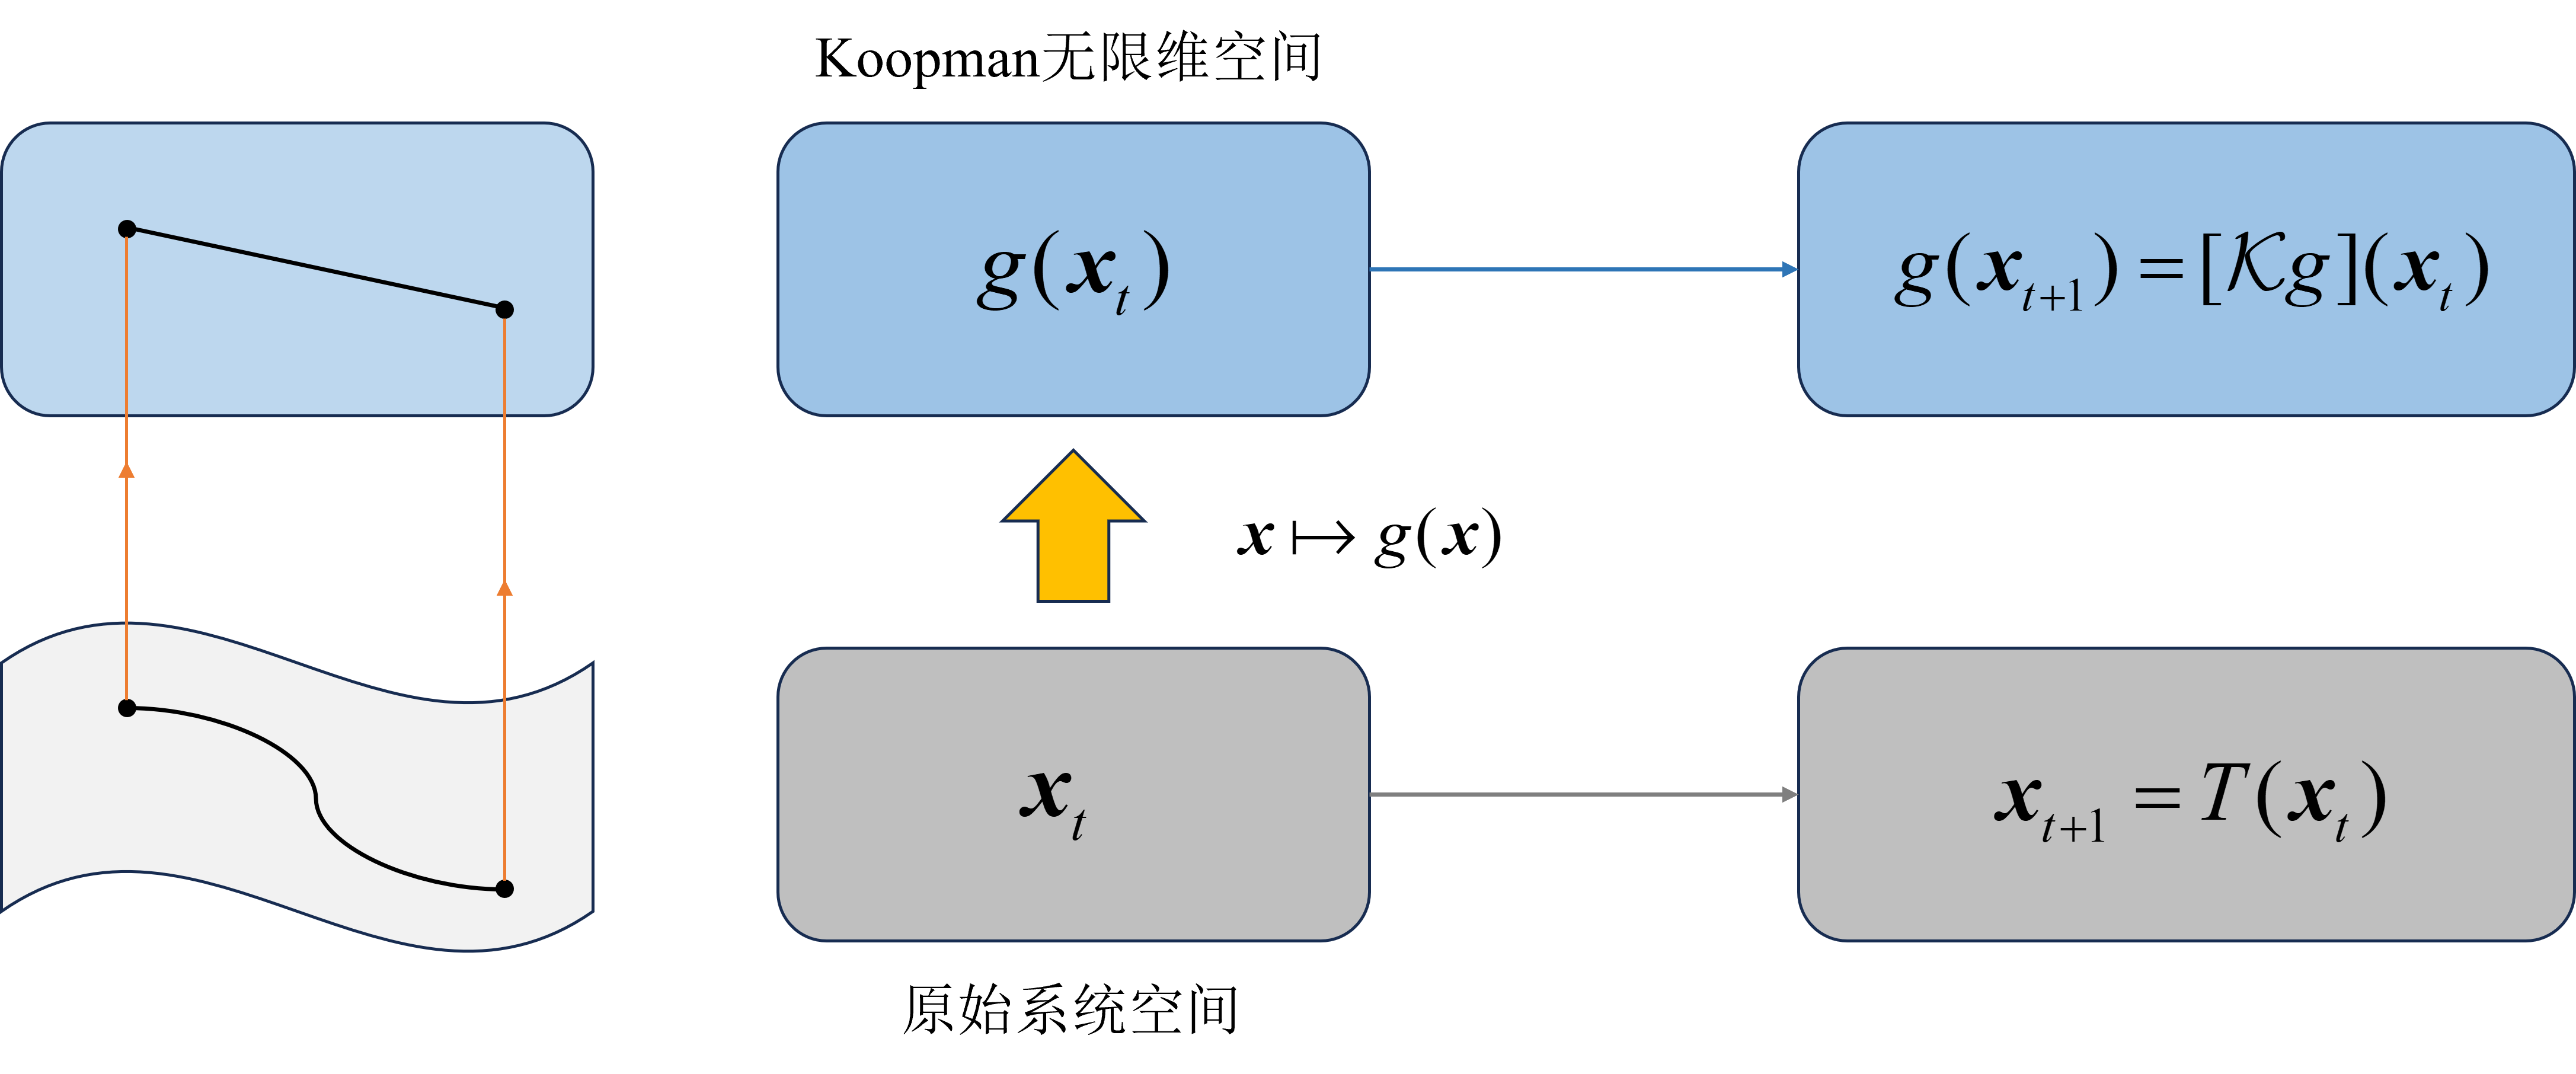
\includegraphics[width=34pc]{picture/3_1.png} 
	\caption{Koopman算子理论} \label{3_1}
\end{figure}
\subsection{基于Koopman理论的数据驱动预测}

考虑一个离散时间的动力学系统:
\begin{equation}
	x_{t+1} = T(x_t)\label{3-2}
\end{equation}

考虑一个复值函数(称为可观测量)的向量空间 \( \mathcal{F} \),其定义域为系统的状态空间。可以将可观测量 \( g \in \mathcal{F} \) 视为映射或提升的状态。使用与式(\ref{3-2})相关的Koopman算子 \( \mathcal{K}: \mathcal{F} \to \mathcal{F} \) 对可观测量 \( g \) 的演化表示为:
\begin{equation}
	\mathcal{K}g = g \circ T, \quad \forall g \in \mathcal{F}
	\label{3-3}
\end{equation}
其中 \( \circ \) 表示函数复合。为了确保 \( \mathcal{K} \) 是良定义的, \( \mathcal{F} \) 必须在 \( T \) 的复合下封闭。如果 \( \mathcal{F} \) 包含特定的预定义函数(如返回完整状态值的函数),这一条件可能迫使 \( \mathcal{F} \) 成为无限维的。Koopman算子根据以下规则将系统向前传播一步:
\begin{equation}
	\mathcal{K}g(x_t) = g \circ T(x_t) = g(T(x_t)) = g(x_{t+1})
	\label{3-4}
\end{equation}

提升状态 \( g(x) \) 本质上将原始(非线性)系统转化为在Koopman空间中演化的线性系统,从而可以设计和实现各种线性控制器(如LQR)。为了避免处理无限维空间,可以使用Koopman算子的有限维表示。因此,在Koopman算子下不变的有限维子空间 \( \mathcal{S} \subset \mathcal{F} \) 起着至关重要的作用。形式上,设 \( \mathcal{S} \subset \mathcal{F} \) 是一个有限维Koopman不变子空间,并将Koopman算子的作用限制在 \( \mathcal{S} \) 上,即 \( \mathcal{K} \rvert_\mathcal{S}: \mathcal{S} \to \mathcal{S} \)。由于 \( \mathcal{S} \) 是有限维的,给定其基,可以将其表示为矩阵。形式上,设 \( \Psi \) 是一个向量值函数,其元素构成 \( \mathcal{S} \) 的基,则存在一个矩阵 \( \mathcal{K} \in \mathbb{C}^{\text{dim}(\mathcal{S}) \times \text{dim}(\mathcal{S})} \),使得:
\begin{equation}
	\mathcal{K}\Psi = \Psi \circ T = \mathcal{K}\Psi
	\label{3-5}
\end{equation}

结合(\ref{3-5})和(\ref{3-4}),可以得到系统轨迹的线性演化,从而使得(\ref{3-2})可以使用线性系统理论的方法,即:
\begin{equation}
	\Psi(x_{t+1}) = \mathcal{K}\Psi(x_t)\label{3-6}
\end{equation}

通过定义 \( z_t := \Psi(x_t) \),(\ref{3-6})可以写成线性形式 \( z_{t+1} = \mathcal{K}z_t \)。如果空间 \( \mathcal{S} \) 包含状态可观测量 \( g_i(x) = x_i \),其中 \( x_i \) 是状态 \( x \) 的第 \( i \) 个元素,则可以选择基 \( \Psi \) 使其包含 \( g_i \) 作为其元素。在这种情况下,提升的线性系统(\ref{3-6})捕获了原始非线性系统(\ref{3-2})的完整信息。此外,矩阵 \( \mathcal{K} \) 的特征分解允许识别Koopman特征函数和特征值。

通常,找到包含所有状态可观测量的精确有限维不变子空间是具有挑战性的(有时是不可能的)。一个流行的解决方法是近似。假设空间 \( F \) 配备了内积,给定任意空间 \( \mathcal{S} \)(不一定是Koopman算子下的不变空间),可以考虑算子 \( P_\mathcal{S} \mathcal{K}: \mathcal{F} \to \mathcal{F} \),其中 \( P_\mathcal{S} \) 是 \( \mathcal{S} \) 上的正交投影算子。对于这个算子,空间 \( \mathcal{S} \) 是通过构造不变的。因此,可以将这个算子的作用限制在 \( \mathcal{S} \) 上,即 \( P_\mathcal{S} \mathcal{K} \rvert_\mathcal{S}: \mathcal{S} \to \mathcal{S} \),并给定 \( \mathcal{S} \) 的基 \( \Psi \),该算子承认矩阵表示:
\begin{equation}
	P_\mathcal{S} \mathcal{K}\Psi = \hat{\mathcal{K}}\Psi
	\label{3-7}
\end{equation}
其中 \( \hat{K} \in \mathbb{C}^{\text{dim}(\mathcal{S}) \times \text{dim}(\mathcal{S})} \)。在这种情况下,可以写出(4)的近似版本如下:
\begin{equation}
	\Psi(x_{t+1}) = [\mathcal{K}\Psi](x_t) \approx [P_\mathcal{S} K\Psi](x_t) = \hat{\mathcal{K}}\Psi(x_t)
	\label{3-8}
\end{equation}

通过定义 \( z_t := \Psi(x_t) \),前述方程可以写成近似线性形式 \( z_{t+1} \approx \hat{\mathcal{K}}z_t \),从而可以使用高效的线性方法来近似系统的行为。在实践中,通常可以访问系统的离散采样测量数据。这可以用于获得无限维Koopman算子的有限维近似矩阵以及这些基于Koopman的组件。

与标准状态空间模型不同,Koopman算子模型了由系统动力学 \( f \) 驱动的函数演化,并且其存在性对于前向完备系统是保证的。由于Koopman算子是作用在函数空间上的算子,因此它通常是无限维的,但关键在于即使动力学 \( f \) 是非线性的,Koopman算子仍然是线性的。因此,如果 \( \phi \) 是与特征值 \( \lambda \in \mathbb{C} \) 相关联的特征函数,则有 \( K\phi = \lambda\phi \)。由此可以看出,特征函数(或特征函数的线性组合)沿着非线性系统(5)的轨迹线性演化:
\begin{equation}
	\phi(x_{k+1}) = \phi(f(x_k)) = (K\phi)(x_k) = \lambda\phi(x_k)
\end{equation}

给定一组特征函数 \(\{\phi_i\}_{i=1}^{n_\phi}\),任何位于这些特征函数张成的空间内的可观测量都可以分解为:
\begin{equation}
	\psi = \sum_i c_i(\psi)\phi_i
\end{equation}
其中 \( c_k(\psi) \) 称为 \( \psi \) 的Koopman模态。于是我们有:
\begin{equation}
	K\psi = \sum_i c_i(\psi)\lambda_i\phi_i
\end{equation}
其中 \( \lambda_i \) 表示 \( \phi_i \) 的特征值。

在后续内容中,下标 \( u \) 用于表示与带有控制输入的系统相对应的组成部分。给定一个带有控制输入的非线性动力学:
\begin{equation}
	x_{k+1} = f_u(x_k, u_k)
\end{equation}

Koopman算子可以以不同的方式定义。在本工作中,我们考虑了文献[22]中的框架。具体来说,记无限控制序列 \( u := \{u_k\}_{\infty}^{k=0} \in l(U) \),其中 \( l(U) \) 表示所有控制序列的空间。增广状态为:
\begin{equation}
	\chi=\begin{bmatrix}x\\u\end{bmatrix}
\end{equation}

系统的动力学被增广为:
\begin{equation}
	F(\chi_k)=\begin{bmatrix}f_u(x_k,u_k(0))\\Su_k\end{bmatrix}
\end{equation}

其中 \( S \) 是左移算子,定义为 \( Su(i) := u(i + 1) \),且 \( u(i) \) 是 \( u \) 的第 \( i \) 个元素的值。在这种设置下,\( u \) 可以被视为从索引 \( i \) 到实际输出 \( u_i \) 的序列映射。值得注意的是,这个动力系统是无限维的但自治的。因此,上述Koopman算子的定义可以直接应用,并且相应的特征函数假设由以下基函数字典张成:
\begin{equation}
	\{\phi_u(x, u)\}_{i=1}^{n_{\phi_u} + n_u} := \{\phi_{u,1}(x), \ldots, \phi_{u,n_{\phi_u}}(x), u(0)\}
\end{equation}

如果这个基函数字典的演化在系统动力学下是封闭的,那么我们有:
\begin{equation}
\begin{aligned}
	z_{k+1}=Az_k+&Bu_k(0)\\u_{k+1}(0)=&u_k(1)
\end{aligned}
\end{equation}
其中 \( z_k := [\phi_{u,1}(x_k), \ldots, \phi_{u,n_{\phi_u}}(x_k)] \),且 \( A \) 和 \( B \) 捕获了Koopman算子。类似地,这些基函数张成的空间内的任何函数都可以通过Koopman模态恢复为:
\begin{equation}
	\psi_u(x, u(0)) = c_u^T \begin{bmatrix} z \\ u(0) \end{bmatrix}
\end{equation}
其中 \( c := [c_{u,1}, c_{u,2}, \ldots, c_{u,n_{\phi_u} + n_u}] \) 是Koopman模态的向量。特别地,我们对系统输出的恒等函数评估的Koopman模态感兴趣。假设我们有 \( n_y \) 个输出,第 \( i \) 个输出的评估为 \( I_{y,i}(y_k) := y_{k,i} \)。通过一些符号的滥用,输出评估的Koopman模态分解为:
\begin{equation}
	y_k = \begin{bmatrix} I_{y,1}(y_k) \\ I_{y,2}(y_k) \\ \vdots \\ I_{y,n_y}(y_k) \end{bmatrix} = \begin{bmatrix} c_{u,1}^T \\ c_{u,2}^T \\ \vdots \\ c_{u,n_y}^T \end{bmatrix} \begin{bmatrix} z \\ u(0) \end{bmatrix} := C_u \begin{bmatrix} z \\ u(0) \end{bmatrix}
\end{equation}
其中 \( C_u \) 堆叠了输出评估的Koopman模态。

总之,Koopman算子理论通过将非线性系统提升到更高维的线性空间,使得复杂的非线性控制问题可以用线性方法进行处理,从而为非线性系统的控制设计提供了一种有效的工具。

\section{模型预测控制方法}

本小节重点阐述模型预测控制(Model Predictive Control,简称MPC)的基本原理及其应用流程,结合鲁棒非线性控制方法和离散化建模,形成适用于四旋翼无人机系统的完整设计框架。从预测模型建立到代价函数设计,再到优化问题求解,MPC为复杂控制问题提供了一种系统化、灵活性强的解决方案。通过系统状态的预测、滚动优化与反馈修正的有机结合,MPC方法在应对系统非线性、不确定性和外部扰动方面表现出显著的优势。


模型预测控制的核心思想是利用系统的数学模型预测未来的动态行为,并通过在线求解优化问题生成控制输入。其主要特性包括:

(1)预测与滚动优化:通过预测系统在未来一段时间内的行为,寻找最优的控制输入序列;仅执行最优序列中的首个输入,并滚动更新预测区间。

(2) 反馈矫正:实时采集反馈信息,用于修正模型误差和外部扰动的影响。

(3)优化问题求解:将控制问题转化为约束优化问题,通过数值算法在线求解。


以一般形式的二阶非线性系统为例,其状态方程和输出方程为:
\begin{equation}
\begin{aligned}
	\dot{x} = f(x, u&)\\
	\quad y = g(x)&
\end{aligned}
 \label{3-19}
\end{equation}
其中,状态变量 $x \in \mathbb{R}^2$,输入变量 $u$,输出变量 $y \in \mathbb{R}^2$。以下按照参考轨迹生成、系统建模和迭代优化三个步骤对控制器设计流程展开说明。

\subsection{参考轨迹}
在实际应用中,控制系统并不总是追求状态快速收敛。例如在进行轨迹追踪任务中,过快的状态变化可能导致跟踪不收敛。类似PID、
滑模控制、反步法等经典控制方法难以实现对预先设计的追踪,而MPC控制方
法可以比较方便地实现这一点。因此,需要为系统设计合理的参考轨迹 $x_\text{ref}$ 和 $u_\text{ref}$ ,使得目标状态 $x_\text{ref}$ 满足以下动态方程:
\begin{equation}
	\dot{x}_\text{ref} = f(x_\text{ref}, u_\text{ref})
	\label{aa}
\end{equation}
参考轨迹的设计不仅依赖于系统动态特性,还需要综合考虑实际任务需求。

\subsection{名义系统建模}

为便于计算和预测,引入名义系统作为实际系统的线性化近似模型。名义系统亦称标称系统,是实际物理系统的近似描述模型,通常用于预测系统在未来一段时间内的动态行为。针对非线性系统,常以平衡点附近的线性化模型作为其近似表达形式,对非线性函数 $f(x, u)$ 进行泰勒展开得:
\begin{equation}
	\dot{x} = f(x_\text{ref}, u_\text{ref}) + A_\text{con} (x - x_\text{ref}) + B_\text{con} (u - u_\text{ref})
	\label{a}
\end{equation}
其中,矩阵 $A_\text{con}$ 和 $B_\text{con}$ 分别为系统的状态和输入的偏导数矩阵:
\begin{equation}
	A_\text{con} = \frac{\partial f(x, u)}{\partial x} \bigg|_{x = x_\text{ref}, u = u_\text{ref}}, \quad B_\text{con} = \frac{\partial f(x, u)}{\partial u} \bigg|_{x = x_\text{ref}, u = u_\text{ref}}
\end{equation}
定义误差变量 $\tilde{x} = x - x_\text{ref}$,$\tilde{u} = u - u_\text{ref}$,将公式(\ref{a})与公式(\ref{aa})相减,可以得到误差动态方程为:
\begin{equation}
	\dot{\tilde{x}} = A_\text{con} \tilde{x} + B_\text{con} \tilde{u}
\end{equation}

在嵌入式控制应用中,系统需离散化以适应数字控制器的计算能力。假设采样周期为 $T$,利用欧拉法对连续时间系统进行离散化处理得到:
\begin{equation}
	\tilde{x}(k+1) = A_\text{dis} \tilde{x}(k) + B_\text{dis} \tilde{u}(k)
\end{equation}
其中$	A_\text{dis} = I + T A_\text{con}$,$ \quad B_\text{dis} = T B_\text{con}$,$T$为采样周期。
进一步构造增广状态向量,令$\varrho(k|t)=\left[\tilde{x}(k|t),\tilde{u}(k-1|t)\right]^\mathrm{T}$,可以得到:
\begin{equation}
	\begin{aligned}\varrho(k+1|&t)=A\varrho(k|t)+B\Delta u(k|t)\\&\sigma(k|t)=C\varrho(k|t)\end{aligned}
\end{equation}
其中
$$A_0=\begin{bmatrix}A_{dis}&B_{dis}\\0&I\end{bmatrix},B_0=\begin{bmatrix}B_{dis}\\I\end{bmatrix},C_0=\begin{bmatrix}C_{dis}&0\end{bmatrix}$$

假设$N_p$为预测周期,$N_c$为控制周期,通过迭代扩展预测模型可得未来 $N_p$ 步的输出序列:
\begin{equation}
	Y=\psi\varrho(k|t)+\kappa\Delta U
\end{equation}
其中$$
\boldsymbol{Y} = 
\left[
	\boldsymbol{\sigma}(k+1|t) , \boldsymbol{\sigma}(k+2|t) , \boldsymbol{\sigma}(k+3|t) , \cdots , \boldsymbol{\sigma}(k+N_p|t)
\right]^\mathrm{T}$$
$$\boldsymbol{\Psi} = 
\left[
	\boldsymbol{C}_0\boldsymbol{A}_0 , \boldsymbol{C}_0\boldsymbol{A}_0^2 , \boldsymbol{C}_0\boldsymbol{A}_0^3 , \cdots , \boldsymbol{C}_0\boldsymbol{A}_0^{N_p}
\right]^\mathrm{T}$$
$$\boldsymbol{\Delta U} = 
\left[
	\Delta u(k|t) , \Delta u(k+1|t) , \Delta u(k+2|t) , \cdots , \Delta u(k+N_c-1|t)
\right]^\mathrm{T}$$
$$\left.\kappa=\left[\begin{array}{ccccc}{C_{0}B_{0}}&{0}&{0}&{\cdots}&{0}\\{C_{0}A_{0}B_{0}}&{C_{0}B_{0}}&{0}&{\cdots}&{0}\\{C_{0}A_{0}^{2}B_{0}}&{C_{0}A_{0}B_{0}}&{C_{0}B_{0}}&{\cdots}&{0}\\{\vdots}&{\vdots}&{\vdots}&{\ddots}&{0,}\\{C_{0}A_{0}^{Np-1}B_{0}}&{C_{0}A_{0}^{Np-2}B_{0}}&{C_{0}A_{0}^{Np-3}B_{0}}&{\cdots}&{C_{0}A_{0}^{Np-Nc}B_{0}}\\\end{array}\right.\right]$$


\subsection{迭代优化}
模型预测控制的核心在于将控制问题转化为优化问题,并利用先进的计算机技术进行实时求解。对于一般非线性系统 (\ref{3-19}),其代价函数通常定义为:
\begin{equation}
	J = (Y - Y_\text{ref})^T Q (Y - Y_\text{ref}) + \Delta U^T R \Delta U + \rho \epsilon^2
\end{equation}
其中 $Q$ 和 $R$ 分别为输出权重矩阵和输入权重矩阵,$\rho$ 为松弛因子。代价函数中的三项分别对应参考轨迹的跟踪性能、对控制输入量进行约束,以及通过松弛因子方便对优化问题的求解。

令 $E = \Psi \xi - Y_{\text{ref}}$,则有:
\begin{equation}
	\begin{aligned}
		Y - Y_{\text{ref}} &= \Psi \xi + \Theta \Delta U + E - \Theta \Delta U 
		\\&= E + \Theta \Delta U
	\end{aligned}
\end{equation}

通过进一步整理,优化问题最终可以将代价函数表示为具有标准形式的二次规划问题:
\begin{equation}
	J_0 = \frac{1}{2} X^T H X + f^T X
\end{equation}

结合约束条件,将优化问题转化为标准形式的二次规划问题:

\begin{equation}
\begin{aligned}
	&\operatorname*{minimize}_{\Delta U,\varepsilon}&& \frac{1}{2}x^{\mathrm{T}}Hx+f^{\mathrm{T}}x  \\
	&\text{subject to}&& \begin{aligned}&Ax\leq b\\
		&A_{eq}x=b_{eq}\end{aligned}  \\
	&&&lb\leq x\leq ub\
\end{aligned}
\label{3-30}
\end{equation}

模型预测控制就是求解形如公式(\ref{3-30})的优化问题来得到控制量,利用快速二次规划算法可在线计算最优控制输入。




\section{基于数据驱动的非线性模型预测控制器设计}
本节详细阐述了所提出框架的原理与实现方法。核心思想是将外力 $\bm{f}_e$ 和力矩 $\bm{\tau}_e$ 建模为动态系统,并通过数据学习其行为。具体来说,提出的框架借助由Koopman算子理论导出的升维线性系统(Lifted Linear System, LLS),以显式方式捕获外力和力矩的动态特性。

\subsection{升维线性系统}
Koopman算子可以从数据中将非线性系统通过数据映射为全局线性系统 \cite{Mamakoukas2023}。这一性质为显式捕获未知非线性动态(如公式(\ref{quadrotordynamics})中的$\bm f_e$和$\bm \tau_e$)提供了一种数据驱动的方法。因此,本文采用这一特性,通过数据驱动的方式学习$\bm f_e$和$\bm \tau_e$。

考虑一个具有控制输入的未知非线性动力学系统: \begin{equation} \dot{\bm{x}} = \bm{f}(\bm{x},\bm{u}) \label{nonlinear_input} \end{equation} 其中$\bm{x} \in \mathbb{R}^n$为系统状态,$\bm{u} \in \mathbb{R}^p$为控制输入。定义一组标量值函数$\bm{g}$作为升维函数,这些函数构成了一个无限维的Hilbert空间$\mathcal{H}$。假设这些升维函数可以表示为: \begin{equation} \bm{g}(\bm{x},\bm{u}) = \bm{\Phi}(\bm{x}) + \bm{L}\bm{u} \end{equation} 其中$\bm{L}$为常数矩阵。在假设控制输入$\bm{u}$ 不会在Hilbert空间 $\mathcal{H}$ 中演化的条件下,公式(\ref{nonlinear_input})中的非线性动力学系统可以重新表述为: \begin{equation} \bm{\Phi}(\bm{x}(t_0+t_s)) = \bm{\mathcal{K}} \bm{g}(\bm{x}(t_0), \bm{u}(t_0)) = \begin{bmatrix} \bm{A} & \bm{B} \end{bmatrix} \begin{bmatrix} \bm{\Phi}(\bm{x}) \ \bm{u} \end{bmatrix}
\label{3-21} \end{equation} 其中,$\bm{x}(t_0+t_s)=\bm{x}(t_0)+\int_{t_0}^{t_0+t_s}\bm{f}(\bm{x},\bm{u}){\mathrm{d}t}$,$t_s$ 为采样时间$t_s$。上述公式描述了升维函数$\bm{g}(\bm{x})$的前向时间演化。令$\bm{z}(t) \triangleq \bm{\Phi}(\bm{x}(t))$,可以将公式(\ref{3-21})改写为: \begin{equation} \bm{z}(t_0 + t_s) = \bm{A}\bm{z}(t_0) + \bm{B}\bm{u}(t_0) \label{lls} \end{equation} 这被称为未知非线性动力学系统 (\ref{nonlinear_input}) 的升维线性系统(Lifted Linear System, LLS)。

如果给定非线性系统(\ref{nonlinear_input})的一组数据序列 $\{(\bm{x}_1,\bm{u}_1),\cdots,(\bm{x}_{T-1},\bm{u}_{T-1}),(\bm{x}_T)\}$,则可以通过求解以下最小二乘优化问题来近似估计矩阵$\bm{A}$和$\bm{B}$:
\begin{equation}
	\bm{A},\bm{B} = \mathop{\arg\min\limits_{\bm{A},\bm{B}}} \Vert \bm{Z}_{2:T} - (\bm{A}\bm{Z}_{1:T-1}+\bm{B}\bm{U}_{1:T-1}) \Vert \label{LS_AB}
\end{equation} 
其中,$\bm{Z}_{1:T-1}= [ \bm{z}_1,\bm{z}_2,\cdots,\bm{z}_{T-1} ]^\mathrm{T}$,$\bm{Z}_{2:T}= [\bm{z}_2,\bm{z}_3,\cdots,\bm{z}_{T}]^\mathrm{T}$,$\bm{U}_{1:T-1}= [\bm{u}_1,\bm{u}_2,\cdots,\bm{u}_{T-1}]^\mathrm{T}$,$\bm{z}_i$ 表示对应于第 $i$ 个样本 $\bm{x}_i\ (i=1,2,\cdots,T)$ 的状态。当$\bm{Z}{1:T-1}$和$\bm{U}{1:T-1}$的序列长度$T$有限时,上述优化问题实际上对Koopman算子进行了有限维近似 \cite{Hao2024}。

公式(\ref{lls})是离散形式,因其由数据驱动推导得到。因此,根据式 (\ref{lls}),未知非线性系统 (\ref{nonlinear_input}) 的连续有限维近似形式可以表示为: 
\begin{equation}
	\left\{ \begin{array}{c}
		\dot{\bm{z}}=\bm{A_c}\bm{z}+\bm{B_c}\bm{u}\\
		\bm{x}=\bm{Cz}\\
	\end{array} \right. \label{lift_linear}
\end{equation}

其中$\bm{A_c}=\log(\bm{A})/t_s$, $\bm{B_c}=\bm{B}/(\int_{0}^{t_s}e^{\bm{A}t}\text{dt})$, $\bm{z} = \bm{\Phi}(\bm{x}):\mathbb{R}^n \rightarrow \mathbb{R}^K$, $K\gg n$, $\bm{u}\in \mathbb{R}^p$, $\bm{A_c} \in \mathbb{R}^{K\times K}$,  $\bm{B_c} \in \mathbb{R}^{K\times p}$, $\bm{C} \in \mathbb{R}^{n\times K}$,$t_s$为采样时间间隔。





\subsection{基于学习的未知外力和力矩捕获方案}
本节提出了一种数据驱动的基于学习的框架,用以捕捉外力 $\bm{f}_e$ 和力矩 $\bm{\tau}_e$ 的未知动态特性。假设外力和力矩的未知动力学系统可描述为以下形式:

\begin{equation}
	\dot{\bm \chi} = \bm{\xi}(\bm \chi,\bm \zeta) \label{dynamics}
\end{equation}
其中 $\bm \chi = [ \bm f_e, \bm \tau_e]^\mathrm{T}$,$\bm{\xi}$ 表示外力和扭矩的未知动态函数,$\bm{\zeta}$ 表示系统的控制输入,通常是四旋翼的状态或部分子状态。$\bm{\zeta}$ 的选择将在后续的实现部分讨论。

如上所述,类似于公式(\ref{dynamics})这样的未知非线性动力学可以通过有限维的升维线性系统(\ref{lift_linear})从数据中捕捉。然而,寻找合适的基函数 $\bm{\Phi}$ 并非易事。因此,本文提出使用深度神经网络(DNN)来近似构造有限维的基函数,其表示形式如下:
\begin{equation}
	\bm{\Phi}(\bm \chi;\bm{\theta}) = W^{L+1}\phi(W^L(...\phi(W^1 \bm \chi...)) \label{dnn}
\end{equation}
其中,$\bm{\theta} = \{W^1, ..., W^{L+1}\}$ 表示网络的权重参数,$\phi$ 是ReLU激活函数。使用深度神经网络的主要动机在于其在函数近似中的强大能力。
为了找到与Koopman算子相关联的基函数,通过最小化以下损失函数来进行训练:
\begin{equation}
	L = \beta_1 L_{\text{recons}} + \beta_2 L_{\text{forward}} + \beta_3 L_{\text{backward}}
\end{equation}
其中 $\beta_1$、$\beta_2$ 和 $\beta_3$ 是正的超参数,分别衡量三种损失函数的权重。三个损失函数 $L_{\text{recons}}$、$L_{\text{forward}}$ 和 $L_{\text{backward}}$ 定义如下:

\textbf{\romannumeral1) 重构损失 $L_{\text{recons}}$}: 非线性系统的状态应从Hilbert空间 $\mathcal{H}$ 中重构。重构损失函数 $L_{\text{recons}}$ 定义为:
\begin{equation}
	L_{\text{recons}}=\Vert \bm{f}_e(t) - \bm{C} \bm{z}(t) \Vert
\end{equation}

\textbf{\romannumeral2) 多步预测损失 $L_{\text{forward}}$ 和 $L_{\text{backward}}$}: 从带有基准控制器的四旋翼无人机系绳吊运系统中采样数据,构建包含 $s$ 条轨迹的数据集 $\{\bm{X}_i \in \mathbb{R}^{n\times m}, \bm{U}_i \in \mathbb{R}^{p \times m}, i=1,\cdots,s\}$。每条轨迹含有 $m$ 个时间步长的数据。训练所需的标签,即每个采样时刻的外力 $\bm{f}_e$ 和力矩 $\bm{\tau}_e$,由四旋翼动力学方程 (\ref{3-1}) 计算得出。

每个采样时刻的+状态可以表示为 $\bm{Z}_i = [\bm{z}_0^i,\cdots,\bm{z}_{m-1}^i]=[\bm{\Phi}(\bm{\chi_{0}}^i),\cdots,\bm{\Phi}(\bm{\chi}_{m-1}^i)]\in \mathbb{R}^{K\times m}$。
通过升维线性系统(\ref{lift_linear}),基于初始状态 $\bm{z}_0^i$ 进行时间前向和后向预测,得到的预测状态分别为$\hat{\bm{Z}}_i^{\text{forward}} = [\hat{\bm{z}}_0^i, \cdots, \hat{\bm{z}}_{m-1}^i]$ 和 $\hat{\bm{Z}}_i^{\text{backward}} = [\hat{\bm{z}}_0^i, \cdots, \hat{\bm{z}}_{m-1}^i]$。


前向和后向预测误差的损失函数定义为:
\begin{equation}
	\begin{aligned}
		L_{\text{forward}} = \sum_{i=1}^{k} \mu_1^{i} {\rm MSE}(\bm{Z_{i}},\hat{\bm{Z_{i}}}^{\text{forward}})  \\
		L_{\text{backward}} = \sum_{i=1}^{k} \mu_2^{i} {\rm MSE}(\bm{Z_{i}},\hat{\bm{Z_{i}}}^{\text{backward}})\label{L2}
	\end{aligned}
\end{equation}
其中 $\mu_1,\mu_2 \in(0,1)$ 为超参数,用于调整损失项的时间步长权重。损失函数(\ref{L2})专注于最小化向前和向后的多步预测误差,这有助于在更长的预测范围内更精确地预测状态。

\subsection{学习动力学的理论保证}
尽管学习得到的动力学模型能够很好地拟合外力与力矩的动态特性,但其预测结果可能存在发散的风险,进而导致外力和力矩估计误差较大。为确保学习动力学的预测误差在全局范围内可控,需要引入一种约束条件对预测误差进行界定。以下定理为学习动力学的预测误差提供了理论上的全局有界性保证。

\begin{theorem}\label{error_boundness}
	假设存在正数 $\alpha_{\bm{\chi}}$ 和 $\alpha_{\bm{\zeta}}$,使得 $\Vert \bm{\chi}(t_0+t_s)-\bm{\chi}(t_0)\Vert \le \alpha_{\bm{\chi}}$ 和 $\Vert \bm{\zeta}(t_0+t_s) - \bm{\zeta}(t_0) \Vert \le \alpha_{\bm{\zeta}}$ 成立,并且近似得到的Koopman算子 $\hat{\bm{\mathcal{K}}}$ 是稳定的,且与其相关的基函数满足Lipschitz常数 $L_{\bm{\Phi}}$,则学习得到的动力学的预测误差是全局有界的。
\end{theorem}
\begin{proof}
	
在时刻 \( t_0 + n\Delta t \),定义基函数在真实状态 \( s(t_0 + n\Delta t) \) 下的真实值为 
$
\Psi(s(t_0 + n\Delta t))$,
其近似解为$
\tilde{\Psi}_n
$,
其中 $ n \in \mathbb{Z}^+ $ 表示向未来推进的时间步数。

局部误差考虑的是模型在单个时间步长内的精度;全局误差考虑的是模型在所有时间步长内的精度。用$e_n$表示由近似的 Koopman 算子 \( \tilde{K}_d \)引起的第 
\( n \)个时间步的局部误差,其假设 Koopman 算子从前一个时间步开始传播基函数的真实值,即:
\begin{equation}
	e_n\equiv\Psi(s(t_0+n\Delta t))-\tilde{K}_d\Psi(s(t_0+(n-1)\Delta t))
	\label{k}
\end{equation}

其假设为 Koopman 算子可以将上一时间步的基函数真实值进行传播。此外,第 \( n \) 个时间步的全局误差记为 $E_n$。它假设Koopman算子从前一个时间步传播基函数的真实值。类似地,我们用$E_n$来表示第\( n \) 个时间步的全局误差:	
\begin{equation}
	E_n\equiv\Psi(s(t_0+n\Delta t))-\tilde{\mathcal{K}}_d^n\Psi(s(t_0))
	\label{kk}
\end{equation}


当 \( n = 1 \) 时,全局误差与局部误差(公式 (\ref{k}))相等。然而需要注意的是,全局误差(公式 (\ref{kk}))并不是局部误差(公式 (\ref{k}))的累积: 
$
E_n \neq \sum_{i=1}^n e_i
$。
我们在图 \ref{3_2} 中展示了局部误差与全局误差之间的区别。

	令$z(x)=\Psi(s(x))$,基于近似Koopman算子 $\hat{\bm{\mathcal{K}}}$ 的预测误差在经历 $n$ 个采样时刻后的全局误差可以表示为:
	\begin{equation}
		\bm{E}_n = \bm{z}(t_0 + nt_s) - \hat{\bm{\mathcal{K}}}^n \bm{z}(t_0)
	\end{equation}


	
	通过递归迭代(\ref{lls}), 全局预测误差可以表示为
	\[
	\begin{aligned}
		\Vert \bm{E_n} \Vert &= \Vert \bm{\Phi}(t_0+nt_s) -\hat{\bm{\mathcal{K}}}^n\bm{\Phi}(t_0) \Vert  \\
		&=\Vert \sum_{i=0}^{n-1}\hat{\bm{\mathcal{K}}}^i\bm{e}(t_0+(n-i)t_s)\Vert \\
		&\le \sum_{i=0}^{n-1}\Vert \hat{\bm{\mathcal{K}}}^i\Vert \cdot \Vert \bm{e}(t_0+(n-i)t_s) \Vert
	\end{aligned}
	\]
	其中,局部预测误差 $\bm{e}(t)=\bm{\hat{\chi}}(t)-\bm{\chi}(t)$,$\bm{\hat{\chi}}$ 表示外部力和力矩的预测值。
	
	由于 $\bm{\chi}$, $\bm{\zeta}$ 和基函数 $\bm{\Phi}$ 是Lipschitz连续的,根据文献\cite{Hao2024}的定理1,局部预测误差 $\bm{e}(t)$ 有界,即
	\[
	\begin{aligned}
		\lim_{n_h\rightarrow \infty} \text{sup} \Vert \bm{e}(t) \Vert &=(\Vert \bm{CA} \Vert L_{\bm{\Phi}}+1) \alpha_{\bm{\chi}}+\Vert \bm{CB}\Vert \alpha_{\bm{\zeta}} \\
		&+\max_{\overline{\bm{\chi}}\in \mathbb{B}} \Vert \overline{\bm{\chi}} -\bm{C}\bm{\Phi(\overline{\bm{\chi}}}) \Vert \triangleq c
	\end{aligned}
	\]
	其中,$n_h$ 是基函数中最后一个隐藏层的层数,$\mathbb{B}$ 是包含每个采样时刻 $\bm{\chi}$ 的集合。由于局部预测误差 $\bm{e}(t)$ 有界,且近似Koopman算子 $\hat{\bm{\mathcal{K}}}$ 稳定,因此
	\[
	\Vert \bm{E_n} \Vert \le \sum_{i=0}^{n-1}\Vert \hat{\bm{\mathcal{K}}}^i\Vert \cdot \Vert \bm{e}(t_0+(n-i)t_s) \Vert\le \Vert c \Vert \sum_{i=0}^{n-1}\Vert \bm{\mathcal{K}}^i \Vert
	\]
	是有界的。即预测误差有界。
\end{proof}


综上所述,上述定理表明,在满足特定条件下,学习的动力学模型的预测误差在全球范围内是有界的,从而保证了模型的稳定性与预测的准确性。
\begin{figure}[hbt!]
	\centering
	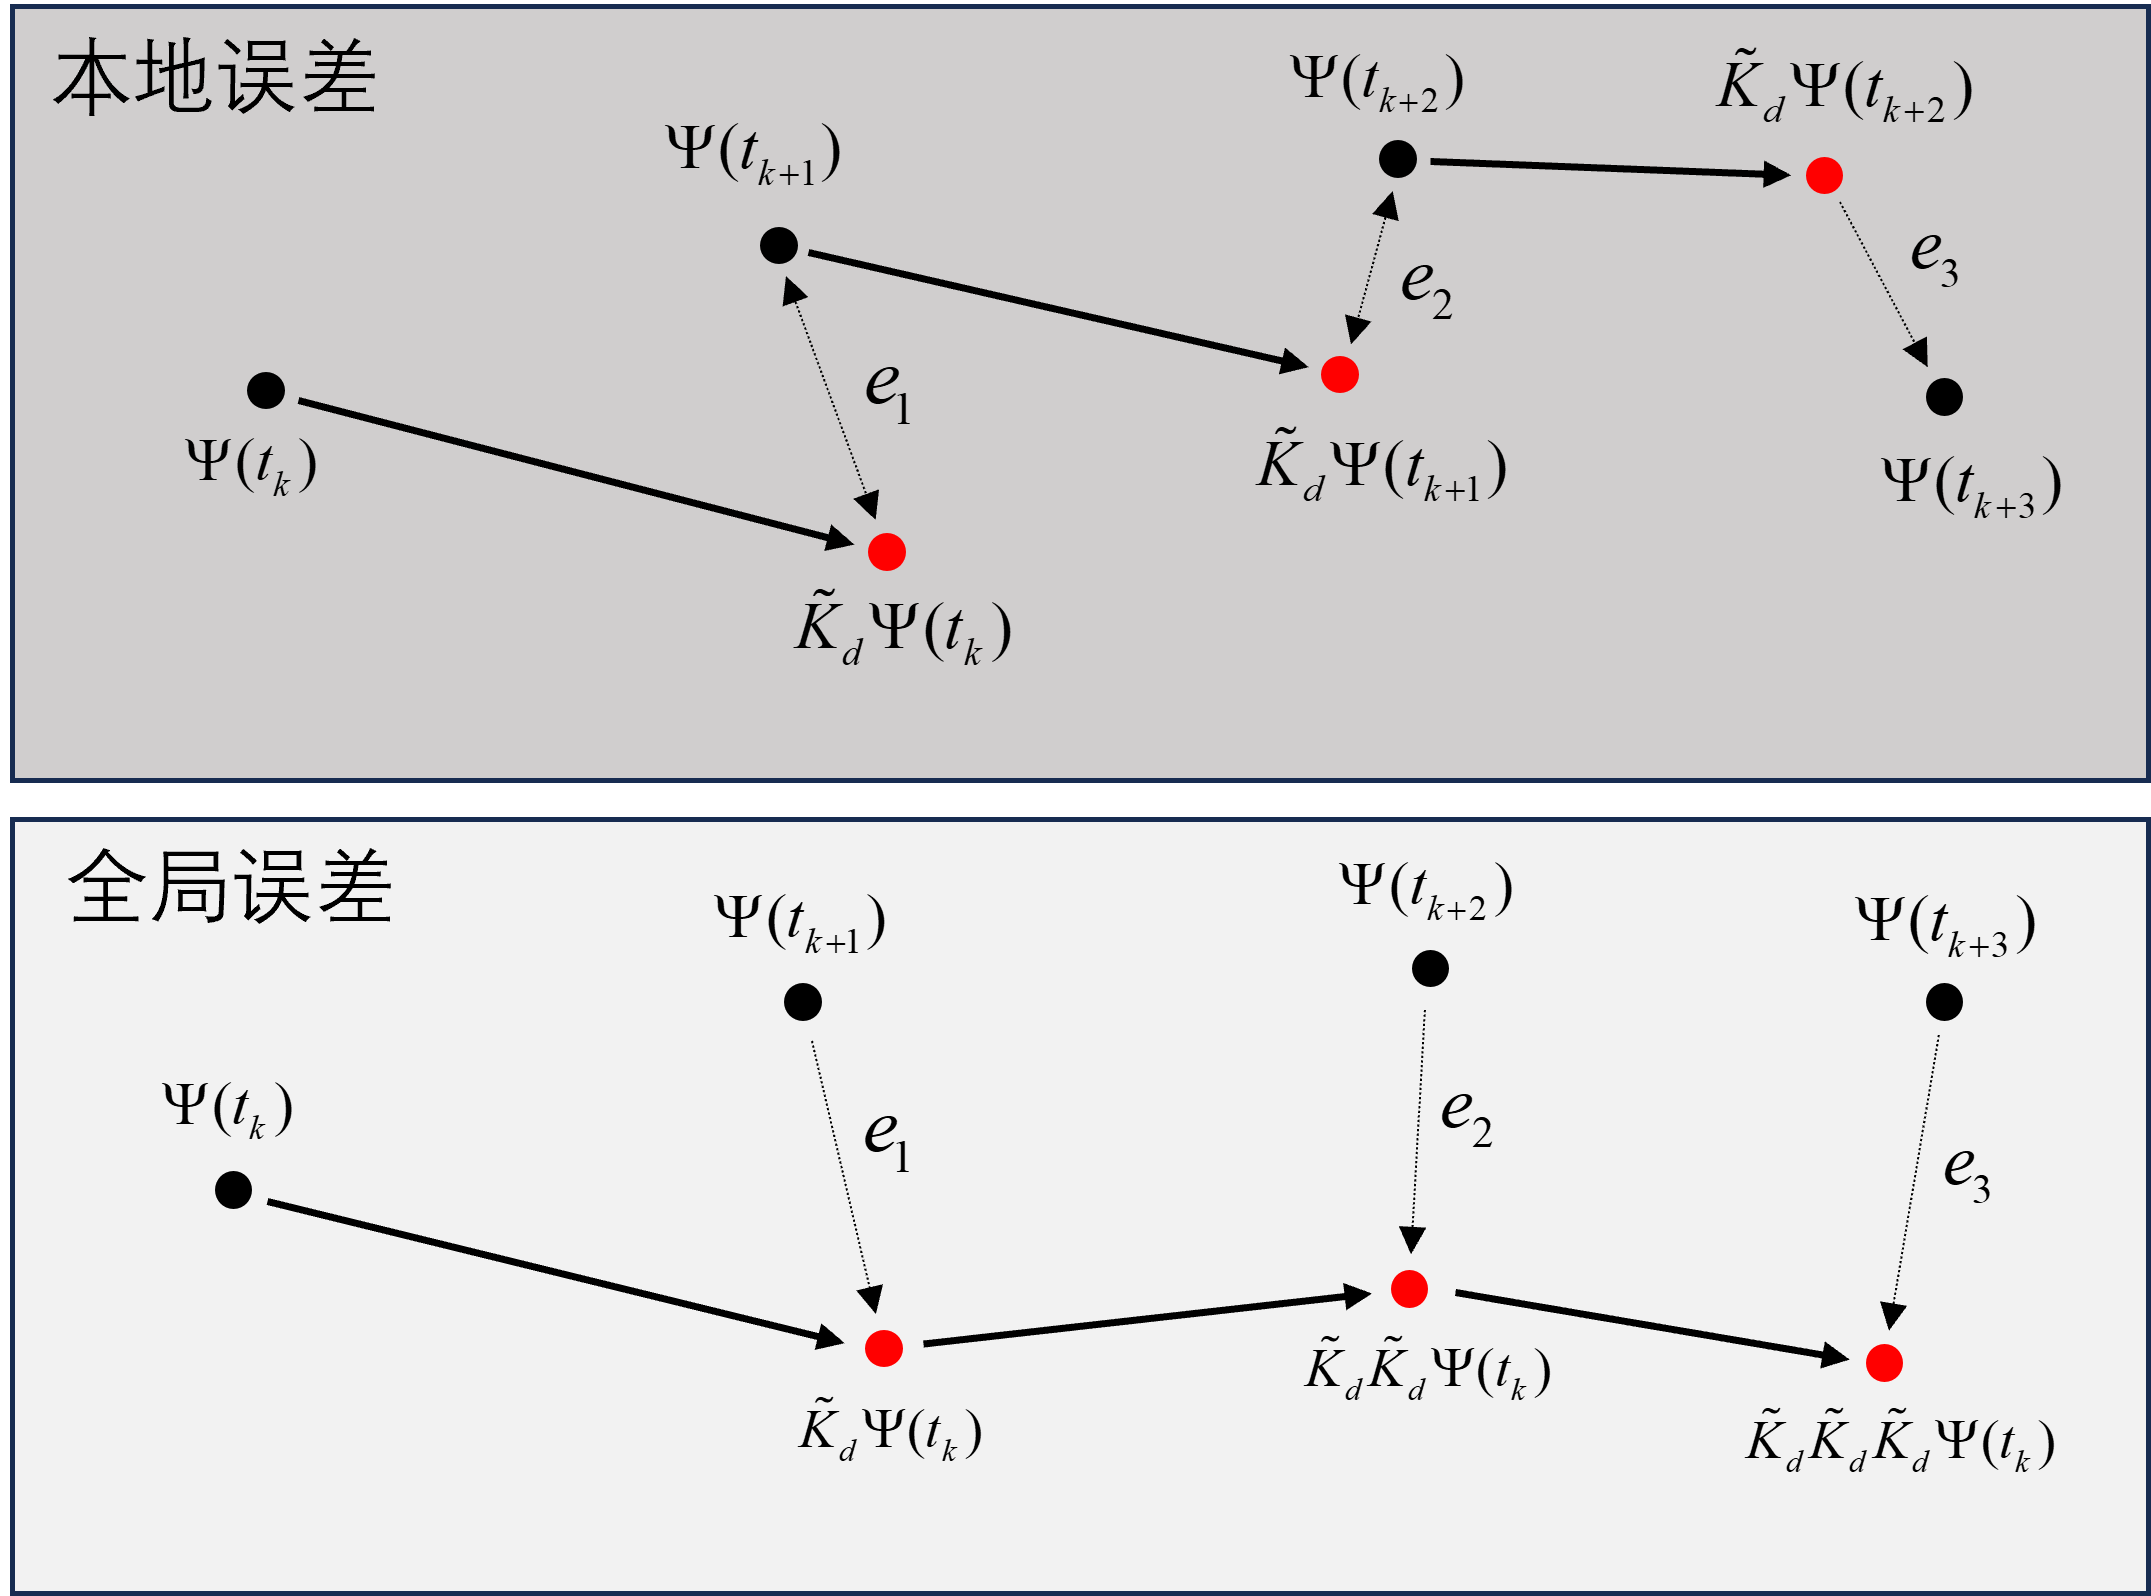
\includegraphics[width=30pc]{picture/3_2.png} 
	\caption{近似Koopman算子引起的局部误差和全局误差} \label{3_2}
\end{figure}
\subsection{基函数的Lipschitz常数约束}

如定理 \ref{error_boundness} 所述,如果基函数 $\bm{\Phi}$ 具有Lipschitz常数时,则预测误差是有界的。为了实现这一目标,用谱归一化(Spectral Normalization, SN)方法来约束基函数 $\bm{\Phi}$ 的Lipschitz常数。

根据定义,函数 $\rho$ 的Lipschitz常数等于其梯度的最大谱范数,即 $\Vert \rho \Vert_{\text{Lip}} = \sup \sigma (\nabla \rho)$。因此,对于由深度神经网络(\ref{dnn})参数化的基函数 $\bm{\Phi}$,可以通过限制每一层的谱范数来限定其Lipschitz常数。

线性层 $g(\bm{x})=\bm{W}\bm{x}$ 的Lipschitz常数为 $\Vert g \Vert_{\text{Lip}} = \sup \sigma(\nabla(g))=\sup \sigma(\bm{W})=\sigma(\bm{W})$。因此,基函数$\bm{\Phi}$的Lipschitz常数可以计算为(利用不等式 $\Vert g_1 \circ g_2 \Vert_{\text{Lip}} \le \Vert g_1 \Vert_{\text{Lip}}\cdot \Vert g_2 \Vert_{\text{Lip}}$):

\[
\begin{aligned}
	\Vert \bm{\Phi}(\bm{\chi}) \Vert_{\text{Lip}} &\le \Vert g^{L+1} \Vert_{\text{Lip}} \cdot \Vert \phi_L \Vert_{\text{Lip}} \cdots \Vert \phi_1 \Vert_{\text{Lip}} \cdot \Vert g_1 \Vert_{\text{Lip}} \\
	&= \prod_{l=1}^{L+1}\sigma(\bm{W}^l)
\end{aligned}
\]
其中,ReLU激活函数的Lipschitz常数为1,即 $\Vert \phi_l \Vert_{\text{Lip}} = 1$。在训练过程中,对每一层的权重 $\bm{W}$ 进行谱归一化可以表示为:

\[
\hat{\bm{W}} = \bm{W} / \sigma(\bm{W}) \cdot \gamma ^{\frac{1}{L+1}}  \label{sn}
\]


\begin{lemma} \label{lemma_lip}
	通过对基函数应用谱归一化(\ref{sn})方法之后,基函数的Lipschitz常数将满足以下约束:
	\[
	\Vert \bm{\Phi}(\bm{\chi}) \Vert_{\text{Lip}}\le \gamma
	\]
	其中,$\gamma$ 是基函数的目标Lipschitz常数。
\end{lemma}

\begin{proof}
	对DNN的每一层应用谱归一化之后,基函数的Lipschitz常数满足
	\[
	\Vert \bm{\Phi}(\bm{\chi}) \Vert_{\text{Lip}} \le \prod_{l=1}^{L+1}\sigma(\hat{\bm{W}}^l) = \prod_{l=1}^{L+1}\gamma^{\frac{1}{L+1}}=\gamma
	\]
	因此,通过谱归一化可以有效约束基函数的Lipschitz常数。
\end{proof}

综上所述,在深度神经网络的训练过程中,引入谱归一化技术不仅能够确保网络的Lipschitz常数满足特定的约束,还能提高模型的稳定性和泛化能力。这种方法在实现对嵌入函数约束的同时,避免了直接优化Lipschitz常数所带来的计算复杂性,从而为动态系统的学习提供了更加稳健的理论支撑。


\subsection{基于数据驱动下的学习动力学的控制器实现}

传统的鲁棒模型预测控制方法虽然能够有效应对系统中的不确定性,但其实际应用往往受到严格假设条件的限制,难以完全满足实际工程需求。此外,模型预测控制的闭环性能在很大程度上依赖于其内部模型的准确性,模型误差可能导致控制效果的下降。

为了解决这些问题,引入数据驱动预测模型的方法,利用其强大的数据拟合能力捕捉系统中难以建模或缺失的动态特性,从而显著提升控制器的整体性能和鲁棒性。
对于四旋翼无人机系绳吊运系统来说,使用基于Koopman理论的升维线性系统,对未知有效载荷和残余动力学引起的外力进行建模,捕获得到未知外力和力矩并集成到模型预测控制框架中,系统的模型以及状态和输入约束被考虑在如下形式的优化问题中:
\begin{equation}
	\begin{aligned} \label{nmpc}
		&\operatorname*{minimize}_{\bm{\bar{u}}}& & \sum_{i=0}^{N-1}\left(\bm{\bar{x}}_i^T\bm{Q}\bm{\bar{x}}_i + \bm{\bar{u}}_i^T\bm{R}\bm{\bar{u}}_i\right) + \bm{\bar{x}}_N^T\bm{P}\bm{\bar{x}}_N  \\
		&\text{subject to}& & \begin{aligned}
			&\bm{\bar{x}}_{0} = \bm{x}_k, \quad \bm{\bar{x}}_{N} \in \mathcal{X}_f, \\
			&\bm{\bar{x}}_{i+1} = \bm{f}_{\text{nominal}}(\bm{\bar{x}}_i, \bm{\bar{u}}_i) + \bm{f}_{\text{learned}},
		\end{aligned} \\
		&&& \bm{\bar{x}}_i \in \mathcal{X}, \quad \bm{\bar{u}}_i \in \mathcal{U}, \quad \forall i = 0, \ldots, N-1
	\end{aligned}
\end{equation}
其中,$\bm{x}_k$表示无人机在时间$k$时刻的状态,$\bm{\bar{x}}_i$和$\bm{\bar{u}}_i$分别是时间$k$的预测状态和控制输入,$N$是预测时域。$\mathcal{X}$、$\mathcal{U}$和$\mathcal{X}_f$分别是状态、控制输入和终端状态的约束集。$\bm{Q}$和$\bm{R}$是状态和控制输入的权重矩阵,$\bm{P}$是终端状态的权重矩阵。$\bm{f}_{\text{nominal}}$是四旋翼无人机的名义动力学,而$\bm{f}_{\text{learned}}$是通过升维线性系统学习得到的动态特性。

该优化问题通过序列二次规划(SQP)求解,并在实时迭代(RTI)方案中使用高斯-牛顿海森近似来提高计算效率。这种方法将学习到的动态特性融合到传统的名义模型里,从而提高控制器的性能和鲁棒性,整个算法的框架如图\ref{illustration_framework}所示,

\begin{figure}[hbt!]
	\centering
	\includegraphics[width=38pc]{picture/3_3.png} 
	\caption{数据驱动下的非线性模型预测控制框架} \label{illustration_framework}
\end{figure}
\section{仿真验证}

\section{神经预测器的性能评估}

在本节中,我们通过数值仿真验证了神经预测器(Neural Predictor)的性能,以证明所提出方案的有效性。升力函数 $\Phi$ 由一个两层的深度神经网络参数化,每层包含128个神经元,激活函数选用ReLU。在所有数值仿真和物理实验中,线性最小二乘法(LLS)的维度 $K$ 被设定为24。我们提出的方案在数值仿真和实际飞行中的实现代码可在以下仓库找到:\href{https://github.com/NPU-RCIR/Neural-Predictor.git}{https://github.com/NPU-RCIR/Neural-Predictor.git}。

在这一部分,我们将神经预测器与最先进的基于学习的估计方法NeuroMHE \cite{NeuroMHE} 和 NeuroBEM \cite{NeuroBEM} 进行了对比,以证明我们所提出方法在捕获外部力/力矩方面的优越性。训练和验证所用数据集与文献 \cite{NeuroBEM} 中提出的 dataset3 相同。神经预测器与NeuroMHE一样采用监督学习进行训练(参见文献 \cite{NeuroMHE} 的第VIIA节)。神经预测器的输入是四旋翼飞行器的线速度和角速度。为了保证公平比较,训练数据集选取了一个10秒长的“摇摆圆轨迹”片段,其速度范围限定在0.19到5.18 m/s,与NeuroMHE中使用的训练数据一致 \cite{NeuroMHE}。在测试阶段,我们同样使用文献 \cite{NeuroMHE} 中所提到的13个未见过的敏捷飞行轨迹来比较神经预测器与NeuroMHE和NeuroBEM的性能。

图2展示了NeuroMHE、NeuroBEM和神经预测器(NP)在一段激烈轨迹(表I中“随机点”,时间段为45s至55s)上的外部力/力矩估计表现。从整体上看,这三种方法都能够准确地估计外部力/力矩。然而,在飞行器执行激烈机动的情况下(图2中的局部放大部分),NeuroMHE和NeuroBEM的外部力/力矩估计效果较差,导致估计性能下降。而我们的神经预测器在该场景下的估计结果更接近真实值,这表明神经预测器在外部力/力矩估计方面仍然保持较高精度。这一优势源于神经预测器将力/力矩建模为一个线性动态系统,并将飞行器状态作为输入。当四旋翼飞行器进行激烈机动时,状态变化驱动神经预测器响应力/力矩的变化,从而实现快速自适应。此外,与最先进的NeuroMHE方法相比,神经预测器在外部力和力矩估计误差上分别显著降低了66.15\%和33.33\%。

为了进一步验证我们方法的有效性,我们在6个未见过的敏捷飞行轨迹上评估了神经预测器的性能。详细结果如表I所示,其中NP表示我们提出的神经预测器。估计误差的均方根误差(RMSE)计算方法与文献 \cite{NeuroMHE} 中的NeuroMHE一致。关于13个未见过的敏捷轨迹的完整比较结果,请参考我们的代码仓库。从结果可以看出,神经预测器在所有情况下均取得了更低的外部力/力矩估计误差,且表现明显优于NeuroMHE和NeuroBEM。在力估计方面,我们的方法在“赛道1”轨迹上将误差最多减少了72.06\%。在力矩估计方面,神经预测器在四个案例中表现优于NeuroMHE和NeuroBEM,且在另外两个案例中表现相当。这些结果表明,神经预测器在许多未见过的激烈飞行轨迹上具有良好的泛化能力,并在外部力/力矩估计方面优于当前最先进的基于学习的估计方法。

为验证所提出方法的样本效率,我们使用1K、2K、3K、4K、5K和6K个样本对神经预测器进行训练,并在测试数据集上评估了估计性能,结果如图3所示。从图中可以看出,随着训练样本量的增加,神经预测器的均方根误差逐渐降低。然而,当训练样本达到4K、5K和6K时,模型在测试集上的表现趋于一致。这表明,4K训练样本已足够揭示外部力/力矩与线速度/角速度之间的动力学关系。此外,与使用4K样本训练的NeuroMHE相比,神经预测器在样本量少于4K的情况下仍表现出较高的性能。具体而言,在力估计任务上,神经预测器达到与NeuroMHE相当的性能时,仅需约1.8K训练样本,大幅减少了训练所需的样本量。

此外,尽管神经预测器是在离线阶段进行训练的,但如前述结果所示,它在外部力/力矩估计中依然具有很强的自适应能力。而由于其训练过程在离线完成,神经预测器在在线执行阶段仅需进行前向推理,显著降低了对机载计算机的计算负担。

综上所述,数值仿真结果表明:
\begin{enumerate}
    \item 所提出的神经预测器能够在飞行器进行激烈机动时快速响应并准确估计外部力/力矩;
    \item 训练后的神经预测器在未见过的敏捷飞行场景下表现出良好的泛化能力和样本效率。
\end{enumerate}


\section{本章总结}




\cleardoublepage

\chapter{多无人机吊运控制}
\chaptermark{多无人机吊运控制}

针对载荷未知的多无人机绳系吊运系统,结合第3章数据驱动的模型预测控制,自动调整控制器的参数并解决各无人机之间的系绳拉力分配问题。基于拉格朗日原理,建立了该系统的动力学方程。在此基础上,结合分布式策略梯度算法,提出了一种新的自适应控制器,在确保系统的稳定性的同时进一步提高跟踪精度。此外,提出了一种基于优化的系绳拉力分配方法,在保障系统稳定性的同时优化了编队的构型。图 \ref{4_1} 展示了该算法的流程图。

\begin{figure}[hbt!]
	\centering
	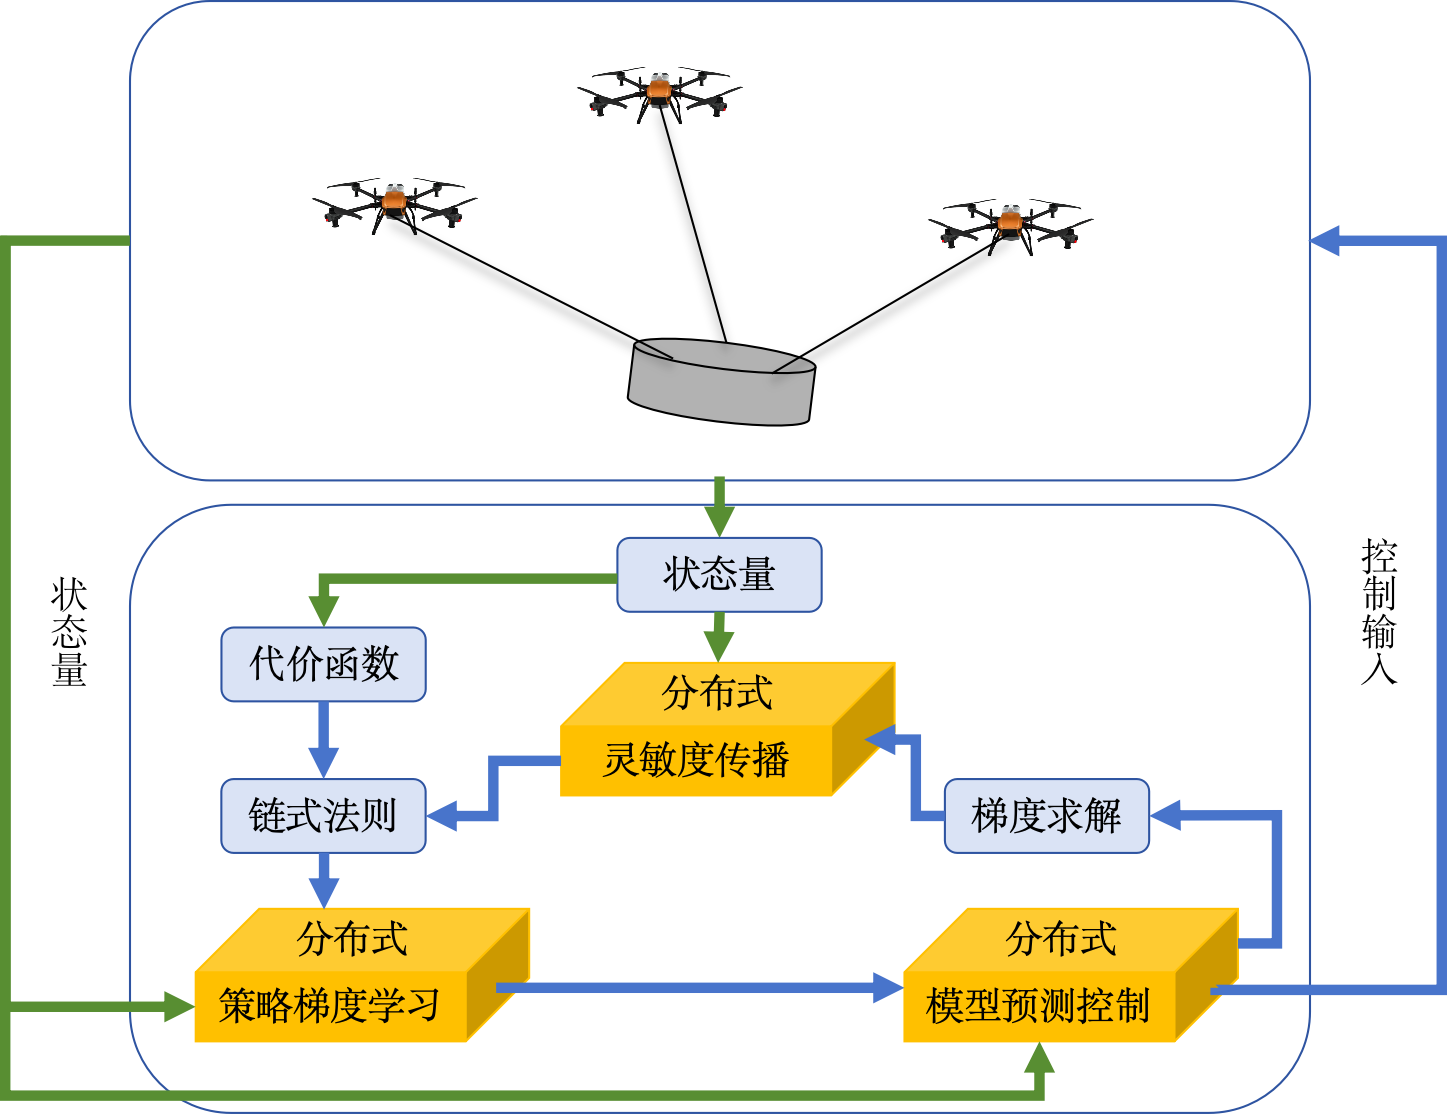
\includegraphics[width=38pc]{picture/4_1.png} 
	\caption{多无人机系统数据驱动控制算法整体框图} 
	\label{4_1}
\end{figure}


\section{问题描述}
考虑 3 架无人机协同运输一个载荷,吊挂载荷通过 3 根等长系绳与多无人机相连,可以通过对第3章的数据驱动的模型预测控制算法进行延伸,应用到本章的多无人机绳系吊运系统中。

对于多无人机系统中,控制策略通常可以分为集中式和分布式两种方式。
集中式控制是指系统的所有无人机都由一个中央控制器进行协调和管理,分布式控制则是让每个无人机根据局部信息和相邻无人机的状态进行决策。集中式控制依赖单一控制中心,本章考虑一种完全分布式的控制方法。
在实际操作中,由于多无人机系统的超参数数量庞大且相互动态耦合,手动调节这些超参数通常既
困难又低效。首先,随着多无人机系统中无人机数量的增加,超参数
的数量也随之增加,从而使调节过程更加复杂。其次,由于通过系绳连接的无人机之间
存在动态耦合,这种耦合效应在载荷具有非均匀质量分布、进行敏捷飞行等情形下会变
得尤为显著。
在这些情况下,无人机之间的拉力分配往往是不均衡且动态变化的,从而需要动态
耦合的模型预测控制权重。此外,模型预测控制的参考轨迹应随着环境和系统状态的变
化而适应系统动态调整的配置,以避免与障碍物发生碰撞。

本章需要解决问题是使用基于数据驱动的分布式、闭环的模型预测控制学习框架来在线动态调整算法参数的权重。这些权重同时在无人机之间以最优的方式对系绳上的张力进行分配,以保持载荷的姿态稳定。

% 在多无人机绳系吊运系统对于给定的任务路径,控制载荷
% 对于多无人机绳系吊运系统,可以对整个
% 将第3章的数据驱动的模型预测控制方法包含在一个集中式 MPC 框架
% 在本章中,

\section{多无人机模型预测控制方法}
我们采用模型预测控制(MPC)来设计多机吊运系统的运动控制与规划策略,目标是跟踪所有无人机(包括载荷)的参考轨迹,并在运输过程中保持载荷的稳定姿态。
\subsection{集中式模型预测控制}


集中式模型预测控制是一种以全局优化为目标的控制策略,适用于多无人机系统的运动控制和路径规划。集中式模型预测控制全局优化能力强,能够协调多主体之间的耦合关系。在本小节中,我们提出了一种集中式的模型预测控制公式,用于为系统生成状态与控制轨迹,并扩展到刚体载荷的情况。

令 \( \bm x_i = \left[ \bm p_i, \bm v_i, \bm q_i, \bm \omega_i \right] \in \mathbb{R}^{13} \) 表示第 \( i \) 个无人机的状态,\( \bm u_i = \left[ f_i, \bm \tau_i \right] \in \mathbb{R}^4 \) 表示第 \( i \) 个无人机的控制,\( \bm x_l = \left[ \bm p_l, \bm v_l, \bm q_l, \bm \omega_l \right] \in \mathbb{R}^{13} \) 表示载荷的状态,\( \bm u_l = \left[ \bar{T}_1, \cdots, \bar{T}_n \right] \in \mathbb{R}^n \) 表示载荷的虚拟控制。需要注意的是,MPC中使用第3章的数据驱动模型预测方法中优化的张力值作为系绳的上的拉力大小(该张力用于开环预测,但并不直接作用于系统,因此 \( \bar{T}_i \) 被视为载荷的虚拟控制量。

集中式 MPC 的代价函数由无人机和载荷的代价函数组成,每个无人机的代价函数以二次形式设计,用于惩罚无人机的状态与控制相较于参考值的偏差。单个无人机的代价函数表示为:
\begin{equation}
	J_i = \frac{1}{2}\sum_{k=0}^{N-1}\left(\bar{\boldsymbol{x}}_{i,k}^T\boldsymbol{Q}_{x_i}\bar{\boldsymbol{x}}_{i,k}+\bar{\boldsymbol{u}}_{i,k}^T\boldsymbol{R}_{x_i}\bar{\boldsymbol{u}}_{i,k}\right)+\frac{1}{2}\bar{\boldsymbol{x}}_{i,N}^T\boldsymbol{P}_{x_i}\bar{\boldsymbol{x}}_{i,N}
	\label{juav}
\end{equation}
其中,$N$ 是预测时域,$\bar{\boldsymbol{x}}_{i,k}$ 和$\bar{\boldsymbol{u}}_{i,k}$ 是时间 $k$ 时刻无人机 $i$ 的预测状态和控制输入,$\boldsymbol{Q}_{x_i}$ 和 $\boldsymbol{R}_{x_i}$ 是无人机$i$ 的状态和控制输入的权重矩阵,$\boldsymbol{P}_{x_i}$ 是无人机$i$ 的终端状态的权重矩阵。

载荷的成本函数与 \( J_i \) 形式相同,定义为:
\begin{equation}
    J_i = \frac{1}{2}\sum_{k=0}^{N-1}\left(\bar{\boldsymbol{x}}_{l,k}^T\boldsymbol{Q}_{x_l}\bar{\boldsymbol{x}}_{l,k}+\bar{\boldsymbol{u}}_{l,k}^T\boldsymbol{R}_{x_l}\bar{\boldsymbol{u}}_{l,k}\right)+\frac{1}{2}\bar{\boldsymbol{x}}_{l,N}^T\boldsymbol{P}_{x_l}\bar{\boldsymbol{x}}_{l,N}
	\label{jpayload}
\end{equation}
其中$\bar{\boldsymbol{x}}_{l,k}$ 和$\bar{\boldsymbol{u}}_{l,k}$ 是时间 $k$ 时刻载荷的预测状态和控制输入,$\boldsymbol{Q}_{x_i}$ 和 $\boldsymbol{R}_{x_i}$ 是载荷的状态和控制输入的权重矩阵,$\boldsymbol{P}_{x_i}$ 是载荷的终端状态的权重矩阵。


基于上述定义,可以将多无人机系统集中式模型预测控制问题表述为:

\begin{equation}
	\begin{aligned} 
	&\operatorname*{minimize}_{X,U}& & J_l(X_l, U_l) + \sum_{i=1}^n J_i(X_i, U_i)  \\
	&\text{subject to}& & \begin{aligned}
& x_i^{k+1} = \bar{f}_i^k(x_i^k, u_i^k, \Delta t; x_l^k, u_l^k), \quad \forall i \in \mathcal{I}_q \\
& x_l^{k+1} = \bar{f}_l^k(x_l^k, u_l^k, \Delta t; x_1^k, \cdots, x_n^k) \\
& x_i^0 = x_i^t, \quad \forall i \in \mathcal{I}_q \\
& x_l^0 = x_l^t \\
& u_i^{\min} \leq u_i^k \leq u_i^{\max}, \quad \forall i \in \mathcal{I}_q \\
& 0 < \bar{T}_i \leq \bar{T}_{\max}, \quad \forall i \in \mathcal{I}_q \\
& \|p_i^k - p_l^k - R_l^k r_i\|^2 = l_0, \quad \forall i \in \mathcal{I}_q \\
& 2d_\text{quad} - \|p_i^k - p_j^k\|^2 < 0, \quad \forall i, j \in \mathcal{I}_q, i \neq j \\
& d_\text{quad} + d_\text{obs} - \|p_i^k - p_\text{obs}\|^2 < 0, \quad \forall i \in \mathcal{I}_q \\
& d_\text{load} + d_\text{obs} - \|p_l^k - p_\text{obs}\|^2 < 0        
	\end{aligned}	
\end{aligned}
\label{multimpc}
\end{equation}
其中,\( X_i = \left[ x_i^0, \cdots, x_i^N \right] \) 和 \( X_l = \left[ x_l^0, \cdots, x_l^N \right] \) 分别表示第 \( i \) 个无人机和载荷的长度为 \( N+1 \) 的状态轨迹,
\( U_i = \left[ u_i^0, \cdots, u_i^{N-1} \right] \) 和 \( U_l = \left[ u_l^0, \cdots, u_l^{N-1} \right] \) 表示相应的控制轨迹,\( X \) 和 \( U \) 是整个系统的状态与控制轨迹集合。

公式 (\ref{multimpc}) 中的约束从上到下分别表示:
无人机与载荷的离散动态方程,载荷张力的虚拟控制 \( u_l \) 用作优化变量;初始条件;
无人机的控制约束;
系绳张力约束,用于保持系绳绷紧;
系绳长度约束,防止无人机与载荷之间的碰撞;
无人机之间的安全距离;
无人机和载荷的障碍物避让约束。

\subsection{分布式模型预测控制}
解决集中式模型预测控制问题 (\ref{multimpc}) 的计算复杂度较高,同时对通信带宽和系统可靠性要求较高,在多无人机绳系吊运系统中扩展性较差,难以满足实时性的需求。为此,提出了一种分布式的模型预测控制方法,该方法通过将问题分解到各个无人机无人机中实现并行计算,从而降低整体计算复杂度并提高系统的扩展性。

在设计分布式模型预测控制时,需要对集中式模型预测控制问题 (\ref{multimpc}) 的特性进行分析。首先,该代价函数具有分离性,因为载荷与无人机的状态和控制变量之间没有直接耦合,因此目标函数可以按每个无人机独立分离,减少耦合度;其次,无人机之间的动力学通过系绳张力(即载荷状态和控制量的函数)以及系绳的长度约束间接耦合;此外,无人机的状态之间的状态仅通过安全间距约束耦合。

这些特点为分布式优化提供了理论依据,基于这些观察,通过将所有其他无人机的模型预测控制轨迹视为单个无人机进行模型预测控制开环预测时的外部信号,可以实现问题的分解。在此基础上,通过独立更新所有模型预测控制的轨迹直至收敛,得以实现分布式形式。

为了有效提升收敛性,将方程 (\ref{multimpc}) 中的约束转换为软约束,并将其引入到代价函数中。同时,受内点法的启发,软约束通过障碍函数表述,使用充分小的障碍参数可逼近原始约束问题。障碍参数 $\gamma > 0$ 控制约束满足程度和计算效率之间的权衡。

软约束的定义如下:

    (1) \textbf{绳索长度约束}:$h_i^k = \|p_{l,i}\|^2 - l_0$;

    (2)\textbf{安全间距约束}:$g_j^k = 2d_{\text{quad}} - \|p_i^k - p_j^k\|^2$;

    (3)\textbf{避障约束}:$g_{o,i}^k = d_{\text{quad}} + d_{\text{obs}} - \|p_i^k - p_{\text{obs}}\|^2$。


上述软约束通过对约束违规情况进行对数函数的惩罚引入到目标函数中。

具体而言,对于第 $i$ 个无人机,其分解后的模型预测控制问题定义如下,其中其他无人机的轨迹 $X_j, \forall j \neq i, X_l$ 和 $U_l$ 被视为外部信号,在开放式预测中保持不变:
\begin{equation}
	\begin{aligned} 
	&\operatorname*{minimize}_{X^i,U^i}& & J_i + \sum_{k=0}^{N} \left( \frac{1}{2\gamma} h_i^k{}^2 - \gamma \sum_{j \neq i} \ln(-g_j^k) + J_{o,i}^k \right)\\
	&\text{subject to}& & \begin{aligned}
& x_i^{k+1} = \bar{f}_i^k(x_i^k, u_i^k, \Delta t; x_l^k, u_l^k) \\
& x_i^0 = x_i^t\\
& u^i_{\text{min}} \leq u^i_k \leq u^i_{\text{max}}		\end{aligned}	
\end{aligned}
\label{multiuav}
\end{equation}
其中
$\gamma \in \mathbb{R}^+$ 为障碍参数,
$h_i^k = \|p_{l,i}\|^2 - l_0$,$p_{l,i}$ 见公式 (4),
$g_j^k = 2d_{\text{quad}} - \|p_i^k - p_j^k\|^2$,
$J_{o,i}^k = -\gamma \ln(-g_{o,i}^k)$,
$g_{o,i}^k = d_{\text{quad}} + d_{\text{obs}} - \|p_i^k - p_{\text{obs}}\|^2$。

对于载荷的分解模型预测控制问题,其轨迹 $X_i, \forall i \in I_q$ 被视为外部信号,问题定义如下:
\begin{equation}
	\begin{aligned} 
	&\operatorname*{minimize}_{X^l, U^l}& & \min_{X_l, U_l} J_l + \sum_{k=0}^{N} \left( \frac{1}{2\gamma} \sum_{i=1}^{n} h_i^k{}^2 + J_{o,l}^k \right)\\
	&\text{subject to}& & \begin{aligned}
& x_l^{k+1} = \bar{f}_l^k(x_l^k, u_l^k, \Delta t; x_1^k, \cdots, x_n^k) \\
& x_l^0 = x_l^t\\
& 0 < u_l^k \leq \bar{T}_{\text{max}}, \forall i \in I_q		\end{aligned}	
\end{aligned}
\label{multipayload}
\end{equation}
其中$J_{o,l}^k = -\gamma \ln(-g_{o,l}^k)$,$g_{o,l}^k = d_{\text{load}} + d_{\text{obs}} - \|p_l^k - p_{\text{obs}}\|^2$。
\begin{algorithm}[h]
	\caption{多提升系统的分布式 模型预测控制}
	\label{alg:mpc_multilift}
	\textbf{输入:} 阈值 $\delta$,最大迭代次数 $k_{\text{max}}$,以及初始条件 $X^i_0$,$U^i_0$,$X^l_0$ 和 $U^l_0$。\\
	\textbf{输出:} $X^i$ 和 $U^i, \forall i \in \mathcal{I}_A$。
	
	\begin{algorithmic}[1]
	\State $k \gets 1$
	\While{$e \geq \delta$ \textbf{且} $k \leq k_{\text{max}}$}
		\For{$i \gets 1$ 到 $n$ \textbf{(并行)}}
			\State 通过外部轨迹求解问题 (10) 计算 $X^i$ 和 $U^i$
			\Statex \quad 基于外部轨迹 
			\Statex \quad $X^j_{k-1}, \forall j \in \mathcal{I}_q, j \neq i$, $X^l_{k-1}$ 和 $U^l_{k-1}$;
			\Statex \quad $\triangleright$ 在每个智能体上运行并发送到中央无人机
		\EndFor
		\State 更新无人机轨迹: $X^i_k \gets X^i$ 和 $U^i_k \gets U^i, \forall i \in \mathcal{I}_q$;
		\State 通过 $X^i_k, \forall i \in \mathcal{I}_q$ 求解问题 (11) 计算 $X^l$ 和 $U^l$
		\State 更新载荷轨迹: $X^l_k \gets X^l, U^l_k \gets U^l$;
		\Statex \quad $\triangleright$ 在中央无人机中运行
		\State 计算误差: $e \gets \max \{ e^i_X, e^i_U \}, \forall i \in \mathcal{I}_A$ 
		\Statex \quad 其中 $e^i_X = \frac{1}{N} \| X^i_k - X^i_{k-1} \|_2$ \textbf{和} 
		\Statex \quad $e^i_U = \frac{1}{N} \| U^i_k - U^i_{k-1} \|_2$;
		\State 更新迭代次数: $k \gets k + 1$;
	\EndWhile
	\end{algorithmic}
\end{algorithm}

分布式模型预测控制由式 (\ref{multiuav}) 和式 (\ref{multipayload}) 组成,迭代求解。设第 $k$ 次迭代时的轨迹为 $X_i^k, U_i^k, X_l^k, U_l^k$。在每个采样时刻 $t$,给定初始条件 $X_i^0, \forall i \in I_q, X_l^0, U_l^0$,通过以下步骤实现分布式求解:

(1) \textbf{并行计算旋翼无人机轨迹}:各旋翼无人机并行求解问题 (10),使用其他无人机的外部轨迹 $X_j^{k-1}, X_l^{k-1}, U_l^{k-1}$ 进行计算。

(2) \textbf{更新旋翼无人机轨迹}:更新得到的新轨迹 $X_i^k, U_i^k$。

(3) \textbf{计算载荷轨迹}:基于更新后的 $X_i^k$ 求解问题 (11),得到 $X_l^k, U_l^k$。

(4) \textbf{误差计算与收敛判断}:计算误差 $e = \max(e_X^i, e_U^i, \forall i \in I_A)$,其中:
    \begin{equation}
        e_X^i = \frac{1}{N} \|X_i^k - X_i^{k-1}\|^2, \quad e_U^i = \frac{1}{N} \|U_i^k - U_i^{k-1}\|^2
    \end{equation}

(5) \textbf{迭代更新}:若误差 $e \geq \delta$ 且迭代次数未超出最大阈值 $k_{\text{max}}$,继续迭代。


由载荷本身缺乏计算能力,随机选择一个旋翼无人机作为 "中心无人机",负责顺序求解式 (\ref{multiuav}) 和式 (\ref{multipayload})。分布式模型预测控制的流程总结如算法 \ref{alg:mpc_multilift} 所示。

\section{自适应学习的控制参数优化}

分布式模型预测控制 如算法 \ref{alg:mpc_multilift} 所述,通过对集中式 模型预测控制 (\ref{multimpc}) 进行近似来提高计算效率。通常,随着阈值 \(\delta\) 的减小和最大迭代次数 \(k_{\text{max}}\) 的增加,这种近似的准确性会得到改善。然而,算法 \ref{alg:mpc_multilift} 的性能(包括预测轨迹的可行性和跟踪精度)依赖于各种超参数的精细调整。这包括选择权重矩阵以及在 (\ref{juav}) 和 (\ref{jpayload}) 中参考轨迹的设计。

为清晰起见,令 \(\theta^i \in \mathbb{R}^{m_i}, \forall i \in \mathcal{I}_q\) 表示第 \(i\) 个无人机的超参数,\(\theta^l \in \mathbb{R}^{m_l}\) 表示载荷的超参数。因此,我们可以将分解后的 模型预测控制 问题参数化为无人机的
$\text{QMPC}_{\theta^i}, \forall i \in \mathcal{I}_q$和载荷的$\text{LMPC}_{\theta^l}$。
对应的 模型预测控制 预测轨迹分别记为
$\xi^{*,i}_{\theta^i} = \{ X^{*,i}_{\theta^i}, U^{*,i}_{\theta^i} \}$和
$\quad \xi^{*,l}_{\theta^l} = \{ X^{*,l}_{\theta^l}, U^{*,l}_{\theta^l} \}$。

要实现动态耦合的模型预测控制权重的调节,仅通过独立调节各个无人机的 模型预测控制 超参数是不太可能的,且单一固定的超参数集无法普遍适用于所有无人机。手动工程通常依赖于保守的假设,例如均匀的拉力分配和准静态飞行,并且是通过反复试验实现的,这会导致性能不是最优。

\subsection{基于深度神经网络的自适应超参数调整方法}



本研究旨在为多机协同提升系统设计自适应的模型预测控制超参数,并开发一种系统化的自动调优方法。由于此类系统的动态行为复杂且难以通过解析模型进行准确描述,使用深度神经网络(DNN)生成控制器的动态权重和参考值,输入特征包括系统状态、障碍物位置等环境信息。数学上,第 \(i\) 个无人机的自适应模型预测控制超参数可表示为:
\begin{equation}
	\label{4-7}
    \boldsymbol{\theta}^i=f_{\boldsymbol{\pi}^i}\left(\boldsymbol{\chi}^i\right),\mathrm{~}\forall i\in\mathcal{I}_A
\end{equation}


其中,\( \bm \pi_i \) 表示第 \(i\) 个DNN的可学习参数,\( \bm \chi_i \) 包含环境观测数据和系统相关信息,例如系统状态与障碍物信息等。研究的核心问题是,通过优化每个无人机(包括载荷)的DNN参数 \( \pi_i^* \),最小化一个由所有无人机的损失函数组成的总体损失函数。该问题可以形式化为以下优化问题:

\begin{equation}
	\label{4-8}
	\begin{aligned} 
	&\operatorname*{minimize}_{\bm{\pi}}& & L^l+\sum_{i=1}^nL^i  \\
	&\text{subject to}& & \begin{aligned}
		&\boldsymbol{x}_{t+1}^i=\bar{\boldsymbol{f}}_t^i\left(\boldsymbol{x}_t^i,\boldsymbol{u}_{0|t}^{*,i},\Delta t;\boldsymbol{x}_t^l,\boldsymbol{u}_{0|t}^{*,l}\right),\forall i\in\mathcal{I}_q\\&\boldsymbol{u}_{0|t}^{*,i}\text{ generated by QMPC}\left(\boldsymbol{\theta}^i\left(\boldsymbol{\varpi}^i\right)\right)\\&\boldsymbol{x}_{t+1}^l=\bar{\boldsymbol{f}}_t^l\left(\boldsymbol{x}_t^l,\boldsymbol{u}_{0|t}^{*,l},\Delta t;\boldsymbol{x}_t^1,\cdots,\boldsymbol{x}_t^n\right)\\&\boldsymbol{u}_{0|t}^{*,l}\text{ generated by LMPC}\left(\boldsymbol{\theta}^l\left(\boldsymbol{\varpi}^l\right)\right)
	\end{aligned} \\
\end{aligned}
\end{equation}


其中,\( {L}_l \) 和 \( {L}_i \) 分别表示载荷和第 \(i\) 个无人机的损失函数,损失基于它们在给定预测时间范围 \( N_c \in \mathbb{R}^+ \) 内的状态变化计算。参数 \( \pi \) 包含了所有无人机的DNN参数 \( \pi_i \)。



\subsection{基于梯度下降的多无人机闭环训练方法}
上述系统动力学基于名义模型,通过虚拟控制输入 \( u_l \) 进行优化,而实际系统动力学则引入了混合张力大小 \( T = \{T_1, \dots, T_n\} \)。由于 \( T \) 的混合特性,实际系统模型是非可微的,因此无法直接用于优化过程。在实际应用中,由于动态耦合特性和任务复杂性,要求控制器参数优
化能够全面评估闭环性能。为了实现这一目标,提出了一种基于梯度下降的闭环训
练框架,结合分布式分布式灵敏度传播算法,高效计
算灵敏度以优化控制器超参数和深度神经网络(DNN)的参数 π。此方法有效克服了传
统开环训练的局限性,为多无人机协同系统的性能优化提供了灵活高效的解决方案。
与传统开环训练不同,闭环策略考虑了实时反馈对系统性能的影响。

本节提出了针对多机协同提升系统的闭环训练框架,其训练问题采用双层结构进行描述。在底层结构中,通过算法 \ref{alg:mpc_multilift} 解决模型预测控制(\ref{4-8})中的分解子问题,实现系统的开环预测。随后,将计算得到的最优控制指令 \( u^*_{i,0|t} \) 和 \( u^*_{l,0|t} \) 应用于名义系统。其中,\( u^*_{i,\cdot|t} \) 表示基于反馈状态 \( x_i^t \) 计算的最优控制轨迹。在上层结构中,通过优化深度神经网络(DNN)参数 \( \pi \),以最小化总损失函数,从而评估系统的闭环性能。

为了突出闭环训练的优越性,我们将其与现有的开环训练方法进行比较。在保持闭环训练中的模型预测控制设置一致的情况下,继续使用公式 (\ref{4-7}) 中定义的自适应模型预测控制超参数,可以将多机协同提升系统的开环训练问题描述为以下形式:

\begin{equation}
	\label{4-9}
\operatorname*{minimize}_{\bm{\pi}}  \bar{\mathcal{L}}_l + \sum_{i=1}^n \bar{\mathcal{L}}_i,
\end{equation}

其中\( \bar{\mathcal{L}}_l \) 和 \( \bar{\mathcal{L}}_i \) 分别表示载荷和第 $i$ 个无人机的损失函数,基于开环预测轨迹 $\xi_l$ 和 $\xi_i$ 进行定义,其预测时间范围为 \( N_\text{ol} \in \mathbb{R}^+ \);
闭环状态 $X^\text{cl}$ 的演化由动态系统 $x_{t+1} = f(x_t, u_t)$ 和最优控制指令 $u^*$ 决定。

相较于开环训练问题(\ref{4-9}),闭环训练问题(\ref{4-8})具有两大主要优势。首先,在闭环训练中,预测范围 \( N_\text{cl} \) 可以超过模型预测控制的预测范围 \( N \),从而提供了更大的训练灵活性,而开环训练中的预测范围\( N_\text{ol} \) 则不能超过 \( N \)。其次,开环训练中的损失函数 \( \bar{\mathcal{L}}_l \) 和 \( \bar{\mathcal{L}}_i \) 依赖于专家示范轨迹 \( \xi_{d,l} \) 和 \( \xi_{d,i} \),这些示范数据往往难以获取,限制了开环训练仅能用于模仿学习。相反,闭环训练中的损失函数 \( \mathcal{L}_l \) 和 \( \mathcal{L}_i \) 可直接基于系统的闭环状态进行评估,支持更广泛的性能指标(如轨迹跟踪性能和避障能力)。

在闭环训练框架下,优化目标是通过梯度下降调整 DNN 参数 $\bm \pi$,以最小化总损失,我们通过梯度下降求解问题(13)。在闭环训练中,每个个体损失函数对其对应DNN参数$\bm \pi_i$的梯度计算可通过链式法则表达为:

\begin{equation}
	\label{4-10}
\frac{\mathrm{d}\mathcal{L}_i}{\mathrm{d}\pi_i} = \frac{\partial \mathcal{L}_i}{\partial X_i^\text{cl}} \cdot \frac{\partial X_i^\text{cl}}{\partial \theta_i} \cdot \frac{\partial \theta_i}{\partial \pi_i}, \quad \forall i \in \mathcal{I}_A,
\end{equation}

其中 \( X_i^\text{cl} = \{x_i^t\}_{t=T}^{T+N_\text{cl}} \) 表示从某个时间步 \( T \in \mathbb{R}^+ \) 开始的闭环状态轨迹, $\theta_i$ 表示第 $i$ 个无人机控制器的模型预测控制超参数, $\pi_i$ 为控制器参数化的DNN参数。
梯度公式的三项分别对应于损失函数相对于闭环状态的显式梯度、闭环状态对模型预测控制超参数的灵敏度、超参数对 DNN 参数的显式梯度。


在公式(\ref{4-10})中,第一项和第三项的梯度可以直接计算,因为个体损失函数和模型预测控制超参数均是闭环状态和DNN参数的显函数。主要挑战在于求解第二项,即闭环状态对模型预测控制超参数的梯度。为了提高运算效率,下一小节将使用分布式灵敏度传播方法,将计算任务分解到各无人机和载荷中并行执行。


\subsection{多无人机分布式灵敏度传播方法}

在多无人机协同控制系统中,由于无人机与载荷之间的系绳张力耦合和无人机间的间接耦合关系,使得系统的灵敏度传播变得复杂且计算代价较高。为了有效解决这一问题,本文结合 \cite{cheng2023difftune} 中的改进梯度优化方法和分布式灵敏度传播算法,提出了一种适用于多无人机系统的分布式灵敏度传播框架,用于控制器参数的高效调优。

\paragraph{动态系统模型}  
系统由 3 个无人机和一个载荷组成,定义如下的离散时间动力学模型:

\begin{equation}
	\begin{aligned}
		x^i_{t+1} &= f^i(x^i_t, u^i_t, x^l_t, u^l_t)\\
x^l_{t+1} &= f^l(x^l_t, u^l_t, x^i_t, u^i_t).
	\end{aligned}
\end{equation}
其中 $x^i_t \in \mathbb{R}^n$ 和 $u^i_t \in \mathbb{R}^m$ 分别为第 $i$ 个无人机的状态与控制输入;$x^l_t \in \mathbb{R}^n$ 和 $u^l_t \in \mathbb{R}^m$ 为载荷的状态与控制输入。
灵敏度表示系统状态对控制器参数的偏导数,定义以下灵敏度矩阵:
\begin{equation}
	X^i_{i,t} = \frac{\partial x^i_t}{\partial \theta_i}
	\label{4-13}
\end{equation}
\begin{equation}
	\label{4-14}
	X^l_{i,t} = \frac{\partial x^i_t}{\partial \theta_l}
\end{equation}
\begin{equation}
	\label{4-15}
	X^i_{l,t} = \frac{\partial x^l_t}{\partial \theta_i}
\end{equation}
\begin{equation}
	\label{4-16}
	X^l_{l,t} = \frac{\partial x^l_t}{\partial \theta_l}
\end{equation}

其中式 (\ref{4-13}) 表示第 $i$ 个无人机的状态对其自身控制器参数 $\theta_i$ 的灵敏度;
式 (\ref{4-14}) 表示第 $i$ 个无人机的状态对载荷控制器参数 $\theta_l$ 的灵敏度;
式 (\ref{4-15}) 表示载荷的状态对第 $i$ 个无人机控制器参数的灵敏度;
式 (\ref{4-16}) 表示载荷的状态对其自身控制器参数 $\theta_l$ 的灵敏度。

闭环训练的关键难点在于计算灵敏度项 $\frac{\partial X_i^\text{cl}}{\partial \theta_i}$,这涉及非线性系统动力学和模型预测控制问题的求导。为提高计算效率,我们引入分布式敏感性传播方法(DSP),将灵敏度的计算任务分解到各无人机和载荷中并行执行,从而降低计算和通信的复杂性。

% 根据系统动力学方程,对灵敏度进行递推传播,得到以下公式:
% \begin{align}
% 	\label{4-17}
% X^i_{i,t+1} &= F^i_t X^i_{i,t} + F^{il}_t X^l_{i,t} + G^i_t U^i_{i,t}, \\\label{4-18}
% X^l_{i,t+1} &= F^i_t X^l_{i,t} + F^{il}_t X^l_{l,t} + G^{il}_t U^l_{l,t}.\\\label{4-19}
% X^i_{l,t+1} &= F^l_t X^i_{l,t} + F^{li}_t X^i_{i,t}, \\\label{4-20}
% X^l_{l,t+1} &= F^l_t X^l_{l,t} + \sum_{i=1}^n F^{li}_t X^i_{l,t} + G^l_t U^l_{l,t}.
% \end{align}

% 其中式 (\ref{4-17}) 和 (\ref{4-18}) 表示第 $i$ 个无人机的状态对其自身控制器参数 $\theta_i$ 的灵敏度;
% 式 (\ref{4-19}) 和 (\ref{4-20}) 表示第 $i$ 个无人机的状态对载荷控制器参数 $\theta_l$ 的灵敏度。 $F^i_t$, $F^{il}_t$, $F^{li}_t$, $F^l_t$ 为动力学方程的Jacobian矩阵,表示系统动力学对状态或控制输入的偏导数,具体形式可通过自动微分或符号微分计算得到。

% 为了高效计算灵敏度,提出了分布式灵敏度传播算法,该方法将灵敏度传播任务划分为各无人机和载荷分别计算.
分布式灵敏度传播方法的核心思想是将负载灵敏度 $\mathbf{X}_{l,t}^l$ 视为外部给定的轨迹,从而允许无人机系统的灵敏度在各自子系统中独立并行传播。具体步骤如下:

(1)并行传播四旋翼灵敏度:在每个无人机中,灵敏度 $\mathbf{X}_{i,t}^i$、$\mathbf{X}_{i,t}^l$ 和 $\mathbf{X}_{l,t}^i$ 可以独立计算,使用负载灵敏度 $\mathbf{X}_{l,t}^{l,k-1}$ 作为输入参数。

(2)集中传播负载灵敏度:无人机灵敏度 $\mathbf{X}_{l,t}^i$ 计算完成后,这些灵敏度会被发送到中央无人机。在中央无人机中,根据方程 (16d) 重新计算负载灵敏度 $\mathbf{X}_{l,t}^l$。

(3)迭代执行:灵敏度的计算和更新通过迭代进行,直到系统误差满足收敛阈值 $\delta$ 或达到最大迭代次数 $k_{\text{max}}$。


通过该方法,可以实现灵敏度的分布式并行传播,同时在中央无人机处处理负载灵敏度的集中计算。具体的算法流程总结如算法 \ref{alg:sensitivity_propagation} 所示。

\begin{algorithm}[h]
    \caption{分布式灵敏度传播算法}
    \label{alg:sensitivity_propagation}
    \textbf{输入:} 阈值 $\delta$,最大迭代次数 $k_{\text{max}}$,系统矩阵 (17), (18), (19),新的控制输入 $\{\bar{U}_t\}_{t=T}^{T+N_{cl}}$,初始条件 $\bar{X}_T^0 = 0$ 和 $\{X_{l,t}^{l,0} = 0\}_{t=T}^{T+N_{cl}}$。\\
    \textbf{输出:} 灵敏度轨迹 $\bar{\mathbf{Y}}_t \, (\forall t = T, \cdots, T+N_{cl})$。

    \begin{algorithmic}[1]
    \State $k \gets 1$
    \While{$e \geq \delta$ \textbf{且} $k \leq k_{\text{max}}$}
        \For{$i \gets 1$ 到 $n$ \textbf{(并行)}}
            \For{$t \gets T$ 到 $T+N_{cl}$}
                \State 计算灵敏度轨迹:$X_{i,t}^i$, $X_{i,t}^l$, $X_{l,t}^i$
                \Statex \quad 基于负载的灵敏度 $X_{l,t}^{l,k-1}$
                \Statex \quad $\triangleright$ 在每个智能体中运行,并发送至中央无人机
            \EndFor
        \EndFor
        \State 更新四旋翼灵敏度:$X_{i,t}^{i,k} \gets X_{i,t}^i$, $X_{l,t}^{l,k} \gets X_{i,t}^l, \forall i \in \mathcal{I}_q$
        \For{$t \gets T$ 到 $T+N_{cl}$}
            \State 计算负载灵敏度 $X_{l,t}^l$,基于四旋翼灵敏度 $X_{i,t}^{i,k}, \forall i \in \mathcal{I}_q$
        \EndFor
        \State 更新负载灵敏度轨迹:$X_{l,t}^{l,k} \gets X_{l,t}^l$
        \Statex \quad $\triangleright$ 在中央无人机中运行
        \State 计算误差: 
        \Statex \quad $e \gets \max \{ e_i^i, e_i^l, e_l^i, e_l^l \}, \forall i \in \mathcal{I}_q$
        \Statex \quad 其中:
        \Statex \quad $e_i^i = \frac{1}{N_{cl}} \sum_{t=T}^{T+N_{cl}} \| X_{i,t}^{i,k} - X_{i,t}^{i,k-1} \|_2^2$;
        \Statex \quad $e_l^i = \frac{1}{N_{cl}} \sum_{t=T}^{T+N_{cl}} \| X_{i,t}^{l,k} - X_{i,t}^{l,k-1} \|_2^2$;
        \Statex \quad $e_i^l = \frac{1}{N_{cl}} \sum_{t=T}^{T+N_{cl}} \| X_{l,t}^{i,k} - X_{l,t}^{i,k-1} \|_2^2$;
        \Statex \quad $e_l^l = \frac{1}{N_{cl}} \sum_{t=T}^{T+N_{cl}} \| X_{l,t}^{l,k} - X_{l,t}^{l,k-1} \|_2^2$。
        \State 更新迭代次数:$k \gets k + 1$
    \EndWhile
    \end{algorithmic}
\end{algorithm}

\subsection{分布式策略梯度学习算法}


通过分布式灵敏度传播算法,可以高效地获得系统的灵敏度矩阵。这些灵敏度进一步用于 \cite{cheng2023difftune} 的无学习率梯度优化方法,以实现对控制器参数的高效调优。

\paragraph{优化更新公式}  
根据灵敏度矩阵 $\frac{\partial x_t}{\partial \theta}$,计算梯度:
\begin{equation}
\nabla_\theta L = \sum_{k=0}^N \frac{\partial L}{\partial x_k} \frac{\partial x_k}{\partial \theta} + \sum_{k=0}^{N-1} \frac{\partial L}{\partial u_k} \frac{\partial u_k}{\partial \theta}.
\end{equation}
通过优化更新控制器参数:
\begin{equation}
\theta \leftarrow P_\Theta(\theta + \epsilon^*),
\end{equation}
其中 $\epsilon^*$ 是通过最小化二次损失预测函数 $L(\theta + \epsilon)$ 得到的最优更新量。

本节提出了一种分布式策略梯度学习算法,用于实现多无人机绳系吊运系统的闭环轨迹跟踪控制与障碍物自主避让功能。该算法通过分布式闭环方式高效训练深度神经网络(DNN)参数 $\pi$,并应用于多吊点系统的轨迹跟踪任务。

轨迹跟踪是多吊点系统在负载传输任务中的常见应用。针对系统配置,可以采用现有的轨迹规划算法(例如最小曲率方法)生成平滑的参考轨迹。为了评估系统的轨迹跟踪性能,我们定义每个无人机(吊点)的闭环跟踪误差损失函数 $L_i$,其形式如下:
\begin{equation}
L_i = \sum_{t=T}^{T+N_{cl}} \| x_i^t - x_{i,\text{ref}}^t \|_W^2, \quad \forall i \in \mathcal{I}_A,  \label{28}
\end{equation}
其中,$x_i^t$ 为第 $i$ 个无人机在实际动力学下的闭环状态,$x_{i,\text{ref}}^t$ 为对应的参考状态,$W$ 是一个正定加权矩阵,$N_{cl}$ 表示预测时间域。

在复杂环境下,障碍物避让是飞行任务的核心需求。虽然可以直接将障碍物约束引入模型预测控制(MPC)问题中,但复杂约束通常会导致求解过程的数值计算难度增加。因此,更为可行的方法是通过学习自适应参考轨迹,使系统能够主动响应障碍物并简化MPC求解过程。

针对障碍物避让问题,我们设计了新的损失函数 $L_i$,用于惩罚无人机与障碍物之间的相对距离,具体形式如下:
\begin{equation}
L_i = \alpha \sum_{t=T}^{T+N_{cl}} \exp\left(-\eta \| p_i^t - p_{\text{obs}} \|^2 \right), \quad \forall i \in \mathcal{I}_A,  
\label{29}
\end{equation}
其中,$\alpha$ 和 $\eta$ 为正数权重系数,$p_i^t$ 和 $p_{\text{obs}}$ 分别表示无人机和障碍物在世界坐标系中的位置。

\begin{algorithm}[h]
    \caption{分布式策略梯度}
    \label{alg:distributed_pg}
    \textbf{输入:} 学习率 $\epsilon$ 和预先规划的参考轨迹 $x_i^{\text{ref}}, \, \forall i \in \mathcal{I}_A$\\
    \textbf{初始化:} $\varpi_0$
    
    \begin{algorithmic}[1]
        \While{$L_{\text{mean}}$ 未收敛}
            \For{$t \gets 0$ 到 $T_{\text{ep}}$ 以 $\Delta t$ 为步长}
                \State \textbf{前向传播:}
                \State 使用(\ref{4-7})求得自适应超参数 $\theta_t^i, \, \forall i \in \mathcal{I}_A$;
                \State 使用算法 \ref{alg:mpc_multilift} 求得 $u_t^{\ast,i}, \, \forall i \in \mathcal{I}_A$;
                \State 使用(\ref{28})、(\ref{29})或两者的组合计算个体损失 $L_t^i, \, \forall i \in \mathcal{I}_A$;
                \For{$i \gets 1$ 到 $n$ \textbf{(并行)}}
                    \State 使用(5)求得 $T_t^{i,i}$;
                    \State 将 $u_t^{\ast,i}$ 和 $-T_t^{i,i}$ 应用于四旋翼实际模型(\ref{2-22}),以更新闭环状态 $x_t^i$;
                \EndFor
                \State 将 $\left\{ T_t^{i,j} \right\}_{j=1}^n$ 应用于载荷实际模型(\ref{2-15}),以更新闭环状态 $x_t^l$;
                
                \State \textbf{反向传播:}
                \For{$i \gets 1$ 到 $n$ \textbf{(并行)}}
                    \State 使用(26)求得四旋翼的 MPC 相关梯度 $\frac{\partial u_t^{\ast,i}}{\partial \theta_t^i}$;$\triangleright$ 在每个智能体上运行并发送到中央智能体
                \EndFor
                \State 使用与(26)类似的梯度求解器,求得载荷的 MPC 相关梯度 $\frac{\partial u_t^{\ast,l}}{\partial \theta_t^l}$;
                \State $\triangleright$ 在中央智能体中运行
                \If{$t \geq N_{\text{cl}}$}
                    \State 通过 $T_{\text{cl}} \gets t - N_{\text{cl}}$ 确定起始步;
                    \State 使用(17)、(18)和(19)求得系统矩阵;
                    \State 使用(\ref{4-10})求得 $dL_t^i, \, \forall i \in \mathcal{I}_A$;
                    \State 使用基于梯度的优化方法更新 $\varpi_t$;
                \Else
                    \State 保持 $\varpi_t$ 不变;
                \EndIf
            \EndFor
            \State 计算 $L_{\text{mean}} = \frac{\Delta t}{T_{\text{ep}}} \sum_{i=1}^n \sum_{k=0}^{T_{\text{ep}}} L_k^i$,作为下一次迭代的训练误差 $\triangleright$ 一个训练周期
        \EndWhile
    \end{algorithmic}
\end{algorithm}


为了提高训练的灵活性和系统的可行性,我们将轨迹跟踪误差损失(式 \ref{28})与障碍物避让损失(式 \ref{29})进行组合。结合这两种损失函数,通过梯度下降法学习最优策略参数 $\pi$。

具体而言,分布式训练过程包括以下步骤:
\begin{enumerate}
    \item 获取MPC相关梯度(通过式 (26));
    \item 计算系统灵敏度(基于算法2);
    \item 利用链式法则(式 (\ref{4-10}))并行更新各无人机的策略参数 $\pi$。
\end{enumerate}

在此基础上,我们将完整的训练流程总结为算法 \ref{alg:distributed_pg} 。每个训练周期的平均损失 $L_{\text{mean}}$ 由所有个体损失函数的总和计算而得,系统动态离散化的时间步长为 $\bar{\Delta t}$,训练周期的时长为 $T_{\text{ep}}$。


\section{仿真验证}
我们通过广泛的仿真实验验证了\textbf{Auto-Multilift}的有效性,实验主要针对不同飞行场景下模型预测控制(MPC)超参数的学习。具体而言,Auto-Multilift展现出以下几个优势:

\begin{enumerate}
    \item \textbf{快速收敛}:所提出的\textbf{分布式灵敏度传播(DSP)}算法在仅需少量迭代的情况下即可实现快速收敛,且收敛速度不受无人机数量的影响。  

    \item \textbf{自适应MPC权重学习}:Auto-Multilift能够根据轨迹跟踪误差直接学习自适应的MPC权重,与现有的开环学习方法相比,大幅提升了训练稳定性和跟踪性能。  

    \item \textbf{动态障碍物穿越}:除了改进MPC权重学习能力外,我们的方法还能够有效学习自适应张力参考值,使多吊点系统在穿越障碍物时能够进行动态重构。
\end{enumerate}

\subsection{仿真中的实际因素建模}

为了提高仿真的真实性,我们考虑了以下几个实际因素:

\paragraph{弹簧阻尼张力模型} 在弹簧阻尼模型~(3) 中,刚度 \( K = 5000 \, \text{N/m} \),阻尼系数 \( c_t = 0.01 \, \text{s} \)。这种高刚度用于反映绳索张力可能发生的突变现象,这是在绳索负载运输中常见的现象,并将在后续仿真中观察到。

\paragraph{四旋翼的控制模型} 四旋翼的控制输入 \( u_i = [f_i, \tau_i] \) 由螺旋桨的转速生成,然而,螺旋桨的速度无法瞬时变化。因此,我们通过以下一阶系统对四旋翼的控制动态进行建模:
\begin{equation}
    \frac{d}{dt} u_i = \frac{1}{\tau_\Omega} \left( u_i^\text{cmd} - u_i \right),
\end{equation}
其中 \( u_i^\text{cmd} \) 为通过求解四旋翼MPC问题(10)所生成的控制指令,\( \tau_\Omega \) 为电机时间常数。在所有仿真实验中,电机时间常数设定为 \( \tau_\Omega = 33 \, \text{ms} \),这一数值参考文献~\cite{ref41}。

\paragraph{系统模型的离散化} 实际动力学模型~(1) 和~(2) 通过四阶Runge-Kutta方法离散化,时间步长为 \( \Delta \bar{t} = 0.01 \, \text{s} \)。而用于MPC的名义模型~(13b) 和~(13d) 采用相同方法,但时间步长设定为 \( \Delta t = 0.02 \, \text{s} \)。这种较大的时间步长是因为控制系统的更新频率通常低于物理系统,主要是为了适应计算资源的限制或算法设计的策略需求。

\subsection{自适应MPC超参数的约束与网络架构}

为了确保MPC超参数 \( \theta_i \) 在物理上合理且计算上受限,我们采用以下参数化形式:
\begin{equation}
    \theta_i = \theta_i^\text{min} + \left( \theta_i^\text{max} - \theta_i^\text{min} \right) \Theta_i, \quad \forall i \in \mathcal{I}_A,
\end{equation}
其中,\( \theta_i^\text{min} \) 和 \( \theta_i^\text{max} \) 分别表示超参数的下限和上限,\( \Theta_i \) 为归一化超参数,范围在 \([0, 1]\) 之间。

这种参数化对于不同类型的超参数 \( \theta_i \) 都是必要的:
\begin{itemize}
    \item 当 \( \theta_i \) 作为MPC代价函数中的权重时,正的下限可以确保权重矩阵的正定性(假设权重矩阵为对角形式)。
    \item 上限可以防止权重无限增大。
    \item 当 \( \theta_i \) 作为MPC中的张力参考时,指定的范围保证了系统参考值的物理可行性。
\end{itemize}

为了生成在线自适应的归一化超参数 \( \Theta_i \),我们使用多层感知器(MLP)网络。该网络的输出层采用\textbf{Sigmoid激活函数},确保输出范围在 \([0, 1]\) 之间。此外,网络包含两个隐藏层,使用\textbf{ReLU激活函数},并在线性层中应用\textbf{谱归一化},以约束层的Lipschitz常数,从而提高网络的鲁棒性和泛化能力~\cite{ref42}。

\subsection{梯度计算与实现}

针对上述参数化,链式法则~(15) 中的梯度计算公式重写为:
\begin{equation}
    \frac{d L_i}{d \pi_i} = \frac{\partial L_i}{\partial X_i^\text{cl}} \cdot \frac{\partial X_i^\text{cl}}{\partial \theta_i} \cdot \frac{\partial \theta_i}{\partial \Theta_i} \cdot \frac{\partial \Theta_i}{\partial \pi_i}, \quad \forall i \in \mathcal{I}_A.
\end{equation}

我们的方法通过Python实现,分布式MPC问题(如算法1所示)使用\textbf{CasADi}框架中的ipopt求解~\cite{ref43}。MLP网络则通过\textbf{PyTorch}构建,并使用Adam优化器进行训练~\cite{ref44, ref45}。

在训练过程中,我们自定义损失函数 \( L_i^\text{pytorch} \) 以适配PyTorch的训练流程,定义如下:
\begin{equation}
    L_i^\text{pytorch} = \frac{d L_i}{d \Theta_i} \Theta_i^\top \Theta_i,
\end{equation}
其中,
\begin{equation}
    \frac{d L_i}{d \Theta_i} \Theta_i^\top = \frac{\partial L_i}{\partial X_i^\text{cl}} X_i^\text{cl,t} \frac{\partial X_i^\text{cl}}{\partial \theta_i} \theta_i^t \frac{\partial \theta_i}{\partial \Theta_i} \Theta_i^t,
\end{equation}
表示 \( L_i \) 对 \( \Theta_i \) 的梯度在当前时间步 \( t \) 的计算结果。这一设计确保了链式法则下的梯度一致性,即:
\begin{equation}
    \frac{d L_i^\text{pytorch}}{d \pi_i} = \frac{d L_i}{d \pi_i}.
\end{equation}


\section{本章总结}
\subsubsection{5. 方法的优点}

结合 DSP 算法的闭环训练框架在以下方面优于传统开环训练方法:
\begin{itemize}
    \item \textbf{灵敏度计算高效}:DSP 算法将灵敏度传播任务分布到各无人机节点,利用并行计算显著降低计算开销;
    \item \textbf{数据通信优化}:各节点仅需传递必要的灵敏度信息,减少了通信量;
    \item \textbf{性能评估全面}:闭环训练直接基于系统的实际闭环状态,支持多种性能指标(如轨迹跟踪和避障);
    \item \textbf{适应复杂任务}:闭环训练结合学习和优化方法,能够处理高动态耦合任务。
\end{itemize}

\begin{itemize}
    \item \textbf{分布式并行计算}:DSP 将灵敏度传播任务分解到每个无人机节点,减少中心节点负担并加速计算。
    \item \textbf{数据通信高效}:各节点仅需传递必要的灵敏度信息,降低了通信开销。
    \item \textbf{可扩展性强}:方法适用于多无人机系统,节点数量增加时计算与通信复杂度增长有限。
    \item \textbf{真实数据兼容性}:灵敏度传播过程中可结合真实传感器数据,提升实际系统性能。
\end{itemize}

本文提出的基于梯度下降的闭环训练方法通过引入分布式灵敏度传播算法,在保持全局性能优化能力的同时,显著提高了多无人机系统的计算效率。该方法适用于多无人机协同任务(如载荷运输、编队飞行等),为复杂系统的闭环控制器设计和优化提供了一种有效工具。


该分布式策略梯度RL算法能够高效实现多吊点系统的\textbf{轨迹跟踪与障碍物避让},并保证了系统在复杂环境中的闭环稳定性和控制性能。

\cleardoublepage

\chapter{物理引擎仿真与试验验证}
\chaptermark{物理引擎仿真与试验验证}
%为验证所提出方法的可行性与有效性,本章对章动目标消旋地面实验系统进行了搭建。实验系统主要由目标章动旋转模拟装置、磁场源、机械臂和计算机组成,通过目标章动模拟装置模拟空间目标的章动旋转运动,通过机械臂抓取磁场源模拟服务星的运动。采用不同消旋轨迹进行了多组实验,记录目标角速度变化情况并对结果进行了比较分析。
为了验证上述提出方法的可行性与有效性,通过物理引擎仿真和试验验证两个方面对设计的算法效果进行评估。数据驱动方法依赖于大量高质量的标注数据来训练模型。然而,在机器人领域,获取真实世界的数据通常面临数据采集成本高、环境限制、数据标注困难等挑战,物理引擎仿真系统,可以在虚拟环境中高效生成大量多样化且精准标注的数据,避免了真实世界收集数据困难的问题。

在物理引擎仿真方面,利用Drake、Gazebo和MuJoCo几种主流仿真平台,搭建四旋翼无人机绳系吊运系统的动力学和环境模型,并模拟其飞行轨迹与响应特性。在试验验证方面,基于实际硬件搭建四旋翼无人机绳系吊运系统,通过物理引擎和真实试验收集的大量数据,在室内场景中完成一系列试验,验证仿真模型的准确性与适用性。本章通过仿真与试验的结合,为四旋翼无人机绳系吊运系统的设计与优化提供科学依据。
\section{物理引擎仿真系统介绍}
在无人机绳系吊运载荷系统的研究中,仿真是通过计算机模拟现实世界现象的过程。不同的仿真器针对不同的现象进行模拟,提供不同程度的真实感,消耗不同的计算资源,并适用于不同的目的。低保真度的仿真器通常需要较少的计算资源,因此常用于快速估计现实世界的行为或模拟系统的某个特定组件。相反,高保真度的仿真器能够在一个或多个方面更准确地估计现实世界的行为。高保真度的常见维度包括动力学模拟的精确性和更高的视觉真实感。

本章选用了几种主流物理仿真平台对无人机绳系吊运系统的深入分析和验证,包括Drake、Gazebo和MuJoCo。这些平台具有高效的物理建模和仿真功能,可以满足复杂动力学系统建模及仿真精度的需求。本节将对仿真系统的构建流程、各平台的特点及其在仿真中的具体应用进行详细介绍。



\subsection{Drake仿真引擎}

Drake 是由麻省理工学院计算机科学与人工智能实验室与丰田研究院联合开发的一款功能强大的开源物理仿真与控制工具,专注于动力学建模、优化及精确控制仿真。它广泛应用于机器人动力学的分析以及控制系统的开发,特别适合研究高自由度系统。Drake 使用高精度数值积分方法,确保动力学计算的准确性,可模拟包括摩擦、接触、空气动力学在内的复杂机器人动力学,并将这些信息传递给高级规划、控制与分析算法。此外,Drake 提供符号计算与解析梯度支持,对于优化控制和建模复杂任务至关重要。

与 Simulink 类似,Drake 强调模块化设计,具备灵活的接口和先进的数学工具,是学术研究和工业应用的理想选择。其高效的优化工具可用于验证控制算法并优化其性能。

Drake 工具箱提供了以下三大核心组件,用于实现高效、灵活的动力学系统建模:

(1)动态系统建模:Drake 的核心功能包括通过多种动力学组件构建系统模型,这些组件涵盖传感器、执行器、估计器和控制器等模块,满足复杂系统建模的需求。

(2)多体运动学与动力学:Drake 支持解析多种运动学模型格式,可对多体系统进行运动学仿真,同时支持接触建模,实现精确的动力学计算。

(3)数学程序求解:Drake 提供统一的接口支持多种数学规划求解器,能够解决复杂的优化问题,包括路径规划、控制优化和系统稳定性分析。

\begin{figure}[hbt!]
	\centering
	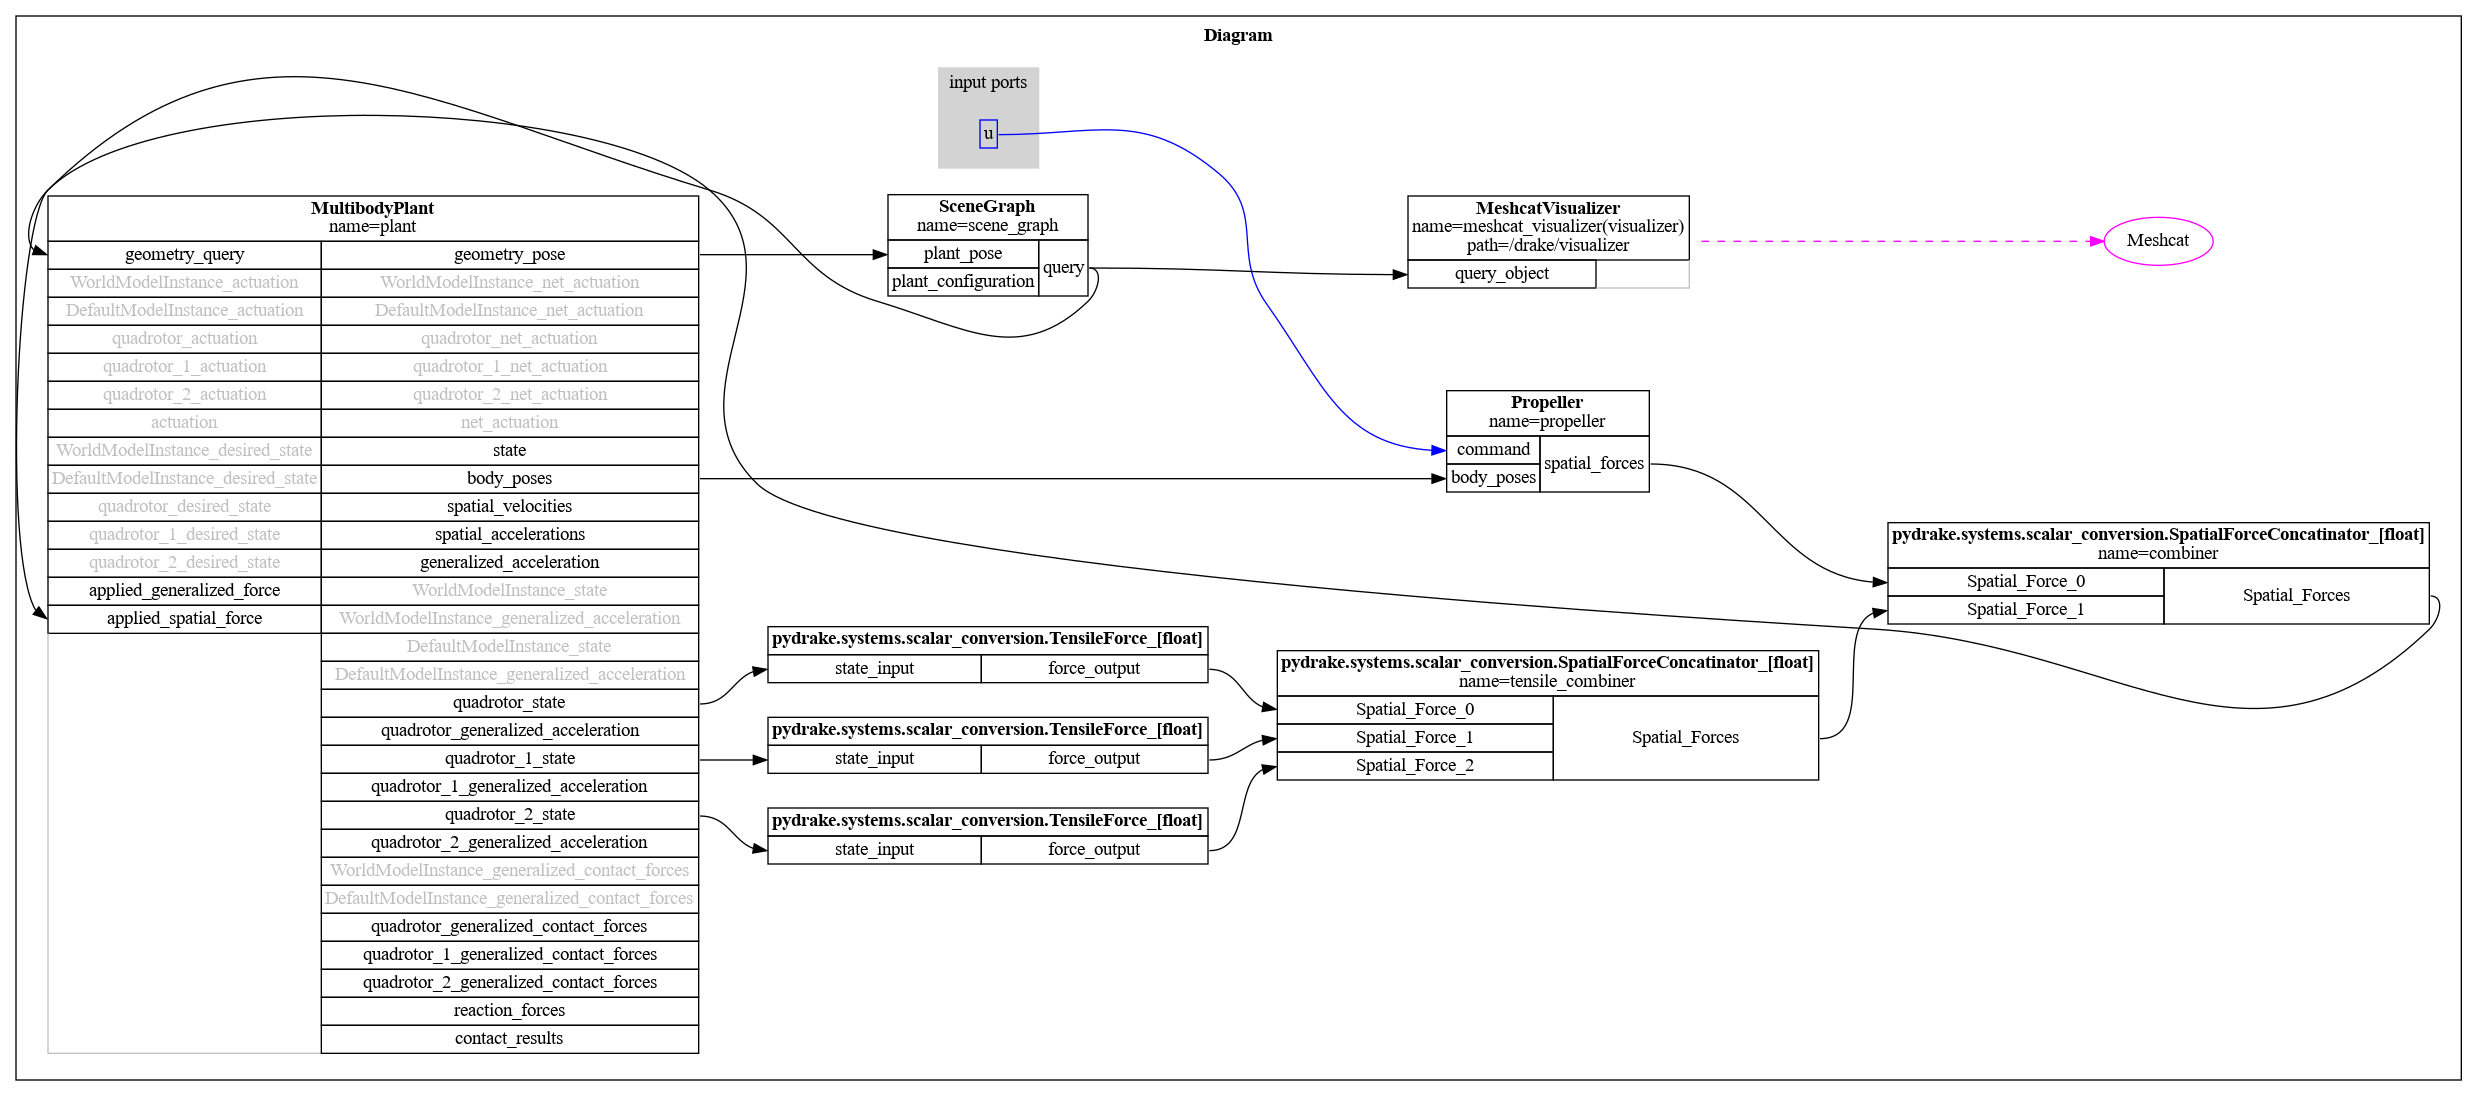
\includegraphics[width=38pc]{picture/drake.png} 
	\caption{Drake仿真引擎中三架无人机系统框图} 
	\label{drake}
\end{figure}
在最初的设计中,无人机绳系吊运系统采用多路复用器和解复用器来拼接系统的输入与输出。然而,这种方法容易导致状态变量之间的混淆问题。为解决此问题,系统设计进行了改进:移除多路复用器和解复用器,直接将三架无人机的 12 个输入传递给系统,并输出三架无人机的所有状态变量。系统的结构如图 \ref{drake} 所示。此外,为每架四旋翼无人机添加了滚转-俯仰-偏航关节。相较于单架无人机的设计,系统中对角权重矩阵 $Q$和控制权重矩阵 $R$的长度增加了三倍,但其组成方式保持不变。

\begin{figure}[hbt!]
	\centering
	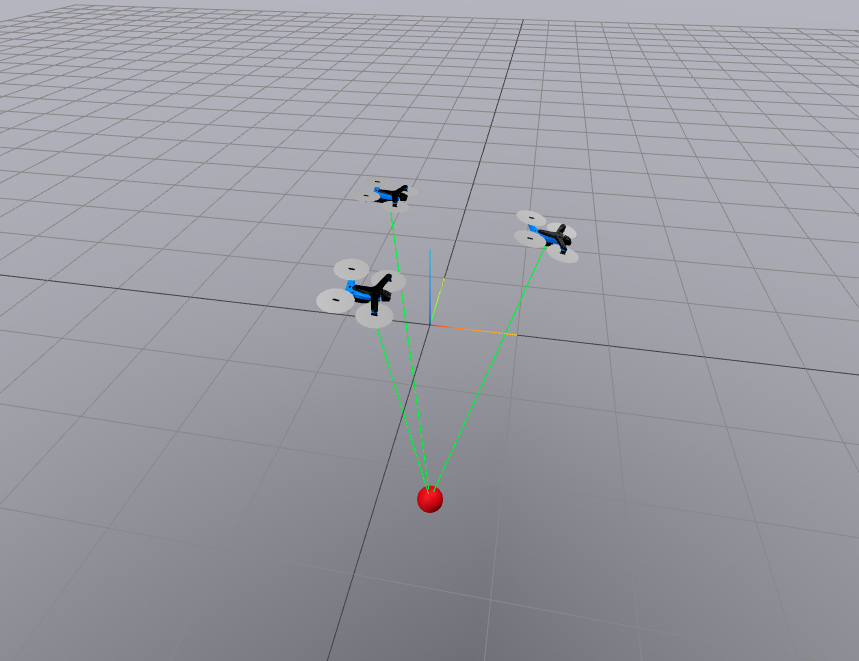
\includegraphics[width=36pc]{picture/5_1.png} 
	\caption{Drake仿真引擎中的多无人机绳系吊运系统} 
	\label{5_1}
\end{figure}

在系统建模过程中,通常使用统一机器人描述格式(URDF)文件,结构化地描述模型的各个部分,并清晰定义系统的动力学属性。在 Drake 中,URDF 文件是主要的建模工具之一,通过定义传感器、执行器和多体结构等实现精确的仿真建模。该系统的动力系统组件还通过增加螺旋桨和控制器模块进一步增强了建模能力。

目前,Drake 主要支持刚体物体的模拟,因此,对于柔性物体如系绳的建模需要采取一定的简化方法。为了解决这一问题,系绳被建模为弹簧,其中弹簧的拉伸会根据系统状态施加力。具体来说,系绳的行为被简化为弹簧模型,在拉紧时,弹簧会施加力,而在松弛时,则不施加任何力。这个方法虽然简化了系绳的物理特性,但依然能够在一定程度上反映系绳在系统中的作用。这样的建模方式引入了系统的混合组件。在系统中,弹簧模型和刚体物体的相互作用形成了一个混合系统。具体来说,当系绳处于拉伸状态时,它会施加弹性力,这与传统的刚体物体动力学行为不同,因此需要将其作为一个特殊的约束条件来处理。尽管 Drake 并不原生支持柔性物体的建模,但通过这种方式,依然能够在仿真中实现系绳的作用,并与其他刚体物体的动力学交互。

此外,Drake 集成了轻量级的 Web 3D 可视化工具 Meshcat,为开发者提供交互式的可视化功能,便于调试、展示与分析仿真结果,如图 \ref{5_1} 所示。通过 Meshcat,开发者可以实时观察复杂系统的运行状态,从而大幅提高开发效率。

\subsection{Gazebo仿真引擎}

因此,如果仿真任务涉及到复杂的物理约束和要求极高的精度,Drake 通常是首选工具。然而,Drake 的缺点在于它的计算复杂度较高,尤其是当仿真规模增大时,计算资源的消耗也随之增加,因此它可能不适合需要快速仿真或大规模环境模拟的场景。

Gazebo 是一个通用的开源仿真框架,它将刚体物理引擎(例如本文使用的开放动力学引擎 ODE)与图形用户界面(GUI)相结合,并提供了丰富的插件,支持复杂的三维环境建模和模拟各种机器人组件(例如电动机、受空气动力学力影响的螺旋桨、传感器噪声以及摄像头等)。类似于 Drake,Gazebo 能够处理通过 SDF 文件定义的多无人机绳系吊运系统,并进行动态交互。
通过与Robot Operating System (ROS) 的集成,可以方便地实现机器人算法的验证和硬件交互仿真。对于四旋翼无人机仿真,Gazebo能够通过插件实现气动力、重力以及绳系约束的精确建模。

然而,Gazebo 与Drake一样,仅能模拟刚体物体。这意味着灵活系绳的动态需要通过多链刚体来进行建模。为此,有五个关键参数可以影响电缆模型的精确度:

(1){链节数量}:每根电缆包含多少个刚性圆柱体。增加链节数有助于使模型更加接近真实电缆,但也需要更多的计算资源。通过经验观察发现,使用 10 个链节足以在配备 i5-1135G7 CPU 和 16 GB 内存的 Intel NUC 计算机上获得足够的精度而不会造成过大计算压力。
    
(2){关节类型}:选择哪种关节类型(例如球形关节、滑动关节或万向节)。由于连续电缆没有刚性关节,最佳选择是约束最少的关节:球形关节。经过多次参数迭代发现,球形关节的阻尼系数不会显著影响关节行为。因此,选择具有功能性阻尼系数的下一个约束最少的关节:万向节。
    
(3) {关节阻尼系数}:描述关节运动过程中能量损失的速率。较大的阻尼系数会导致电缆中的能量传输减少,而过小的阻尼系数则可能导致不稳定的连续振荡。实验表明,$0.01 N s m^{-1}$
的阻尼系数是最优的。若低于此值(即为零阻尼),电缆会振荡至不稳定状态;若高于此值,电缆的运动传递则不如预期。
    
(4){关节摩擦系数}:描述运动关节需要克服的力。由于灵活电缆本身没有刚性关节,加入任何摩擦系数会使电缆模型变得过于刚性。因此,摩擦系数被设为 0。
    
(5) {碰撞几何体}:每个元素的碰撞检测应位于何处。考虑到无人机的配置以及准静态的操作方式,电缆与其他世界元素之间几乎没有碰撞发生。唯一的例外是在飞行前与地面平面的碰撞。由于碰撞建模计算开销较大,而电缆在任何显著情况下都不会发生碰撞,因此电缆的碰撞几何体被禁用。



\begin{figure}[hbt!]
	\centering
	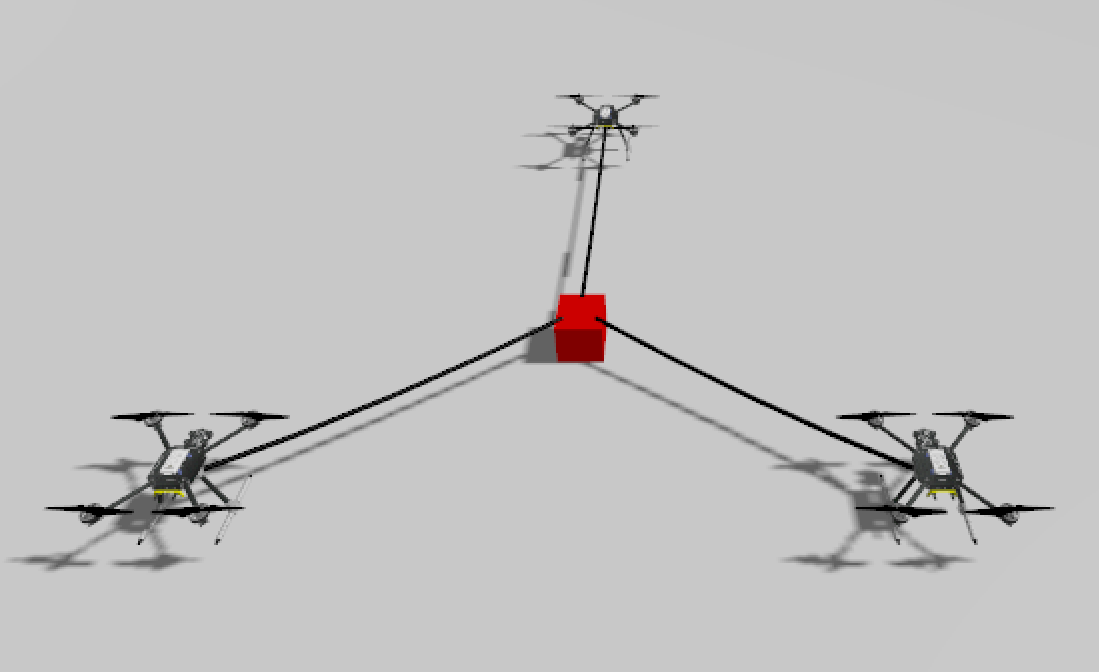
\includegraphics[width=36pc]{picture/5_2.png} 
	\caption{Gazebo仿真引擎中的多无人机绳系吊运系统} 
	\label{5_2}
\end{figure}

图 \ref{5_2} 显示了用于三架无人机和载荷系统的完整 SDF 模型。该模型有三根系绳,每根系绳都是使用离散的链接刚体,两端用球形接头连接。每根系绳都由 XACRO 文件生成,因此可以轻松更改长度、质量和链接数。载荷被模拟为一个球体,系绳连接点沿中心平面对称分布,以模拟载荷的刚体方面。系绳连接到无人机的质量中心。

\begin{figure}[hbt!]
	\centering
	\begin{subfigure}[t]{0.9\textwidth}
		\centering
		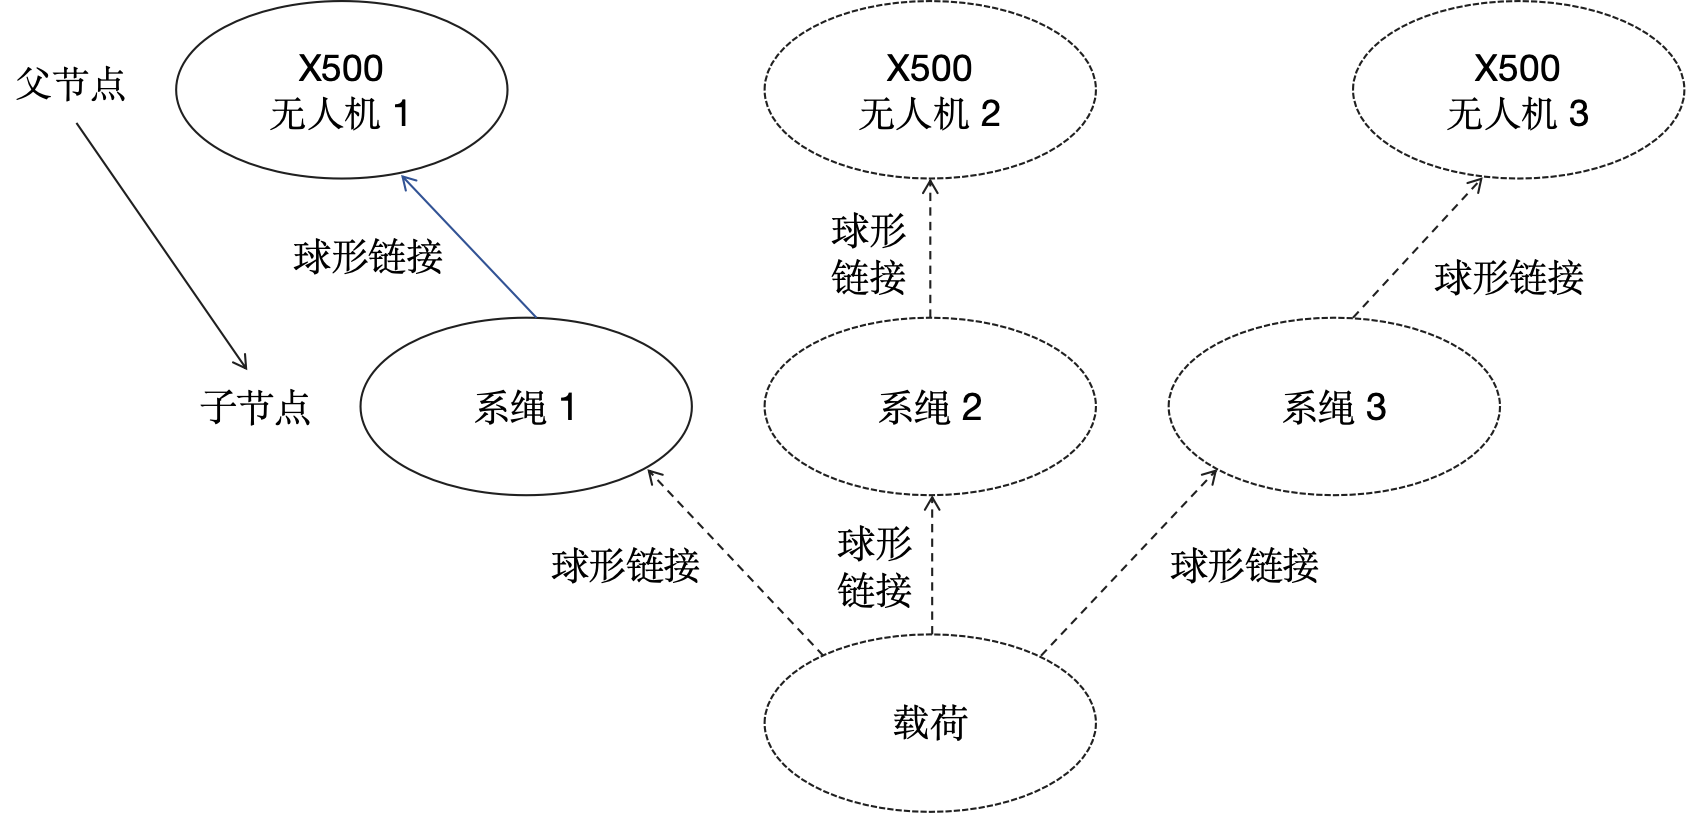
\includegraphics[width=\textwidth]{picture/tree2.png}
		\caption{无人机为父节点}
		\label{tree1}
	\end{subfigure}\\[2ex] % 使得两图之间有一点间距
	\begin{subfigure}[t]{0.9\textwidth}
		\centering
		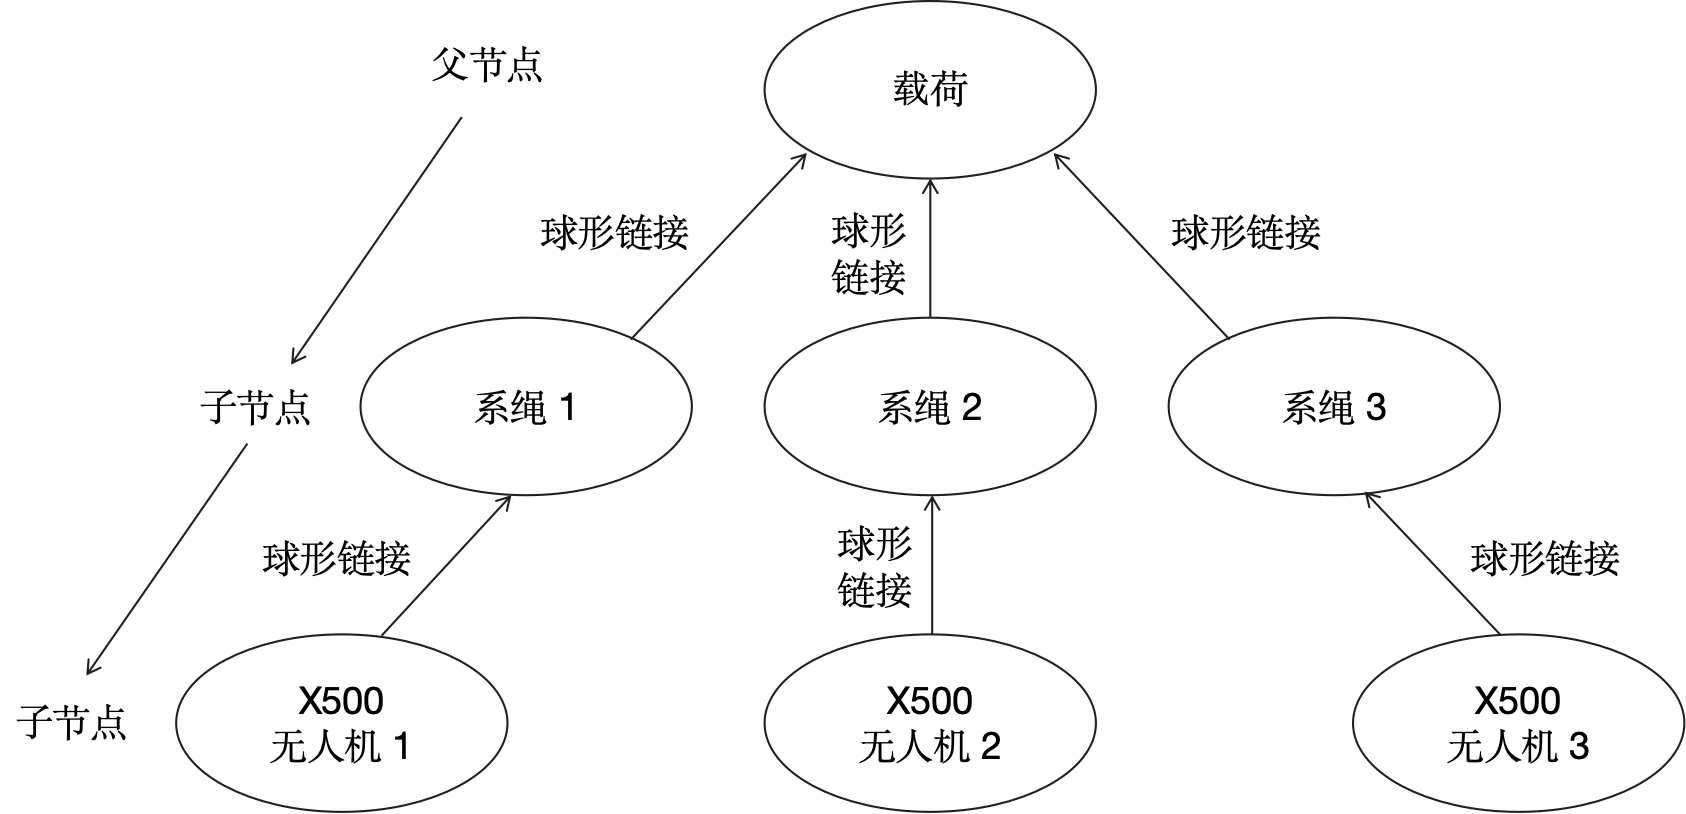
\includegraphics[width=\textwidth]{picture/tree1.png}
		\caption{载荷为父节点}
		\label{tree2}
	\end{subfigure}
	\caption{由无人机、系绳和载荷构成的树图}
	\label{tree_combined}
\end{figure}

将载荷和系绳加入仿真中是一个非常具有挑战性的任务,目前尚未完全解决。在SDF(Simulation Description Format)文件中,"父亲"(parent)通常指的是在运动学树中处于上层的节点(link),它是其他节点的基准或连接点。在SDF文件中,物体的层级结构通过父子节点关系来定义,其中父节点是连接子节点的上级元素。
具体来说,SDF文件中的父子关系可以通过定义<parent>和<child>标签来表示。每个节点(link)都可以定义一个父节点,而该父节点则为其提供参考系或坐标系。在运动学树中,父节点是控制整个系统运动的核心元素,而子节点则通过关节(joint)与父节点相连,从而形成多体动力学系统。系绳原本由多个链接组成,但被简化为一个单一的链接,端部使用球形铰链连接。系绳连接到无人机的质量中心。

对于多无人机绳系吊运系统来说,首先设置父节点为无人机,子节点为系绳和载荷(见图 \ref{tree1})。这是采用类似倒车摆的方式来解决问题,且该方法在网上有较为完善的文档。但是在多无人机绳系吊运系统中,由于多个无人机的存在,只能实现单无人机的绳系吊运系统,当添加负载和另外两架无人机时,遇到了错误(用虚线表示)。
因此,设置载荷为父节点,随后是缆绳和无人机作为子节点(见图 \ref{tree2}),从而构建得到完整的无人机绳系吊运系统SDF文件。

尽管这种离散的电缆模型对于本仿真器来说足够真实,但它仍然不能完全准确地表示真实的柔性电缆。这也突显了寻找一种既精确又计算开销低的电缆动态建模方法的必要性。

在 Gazebo 仿真环境中集成了开源无人机飞控系统 PX4,可以通过 SITL(Software In The Loop)仿真模式进行测试。SITL 仿真指将编译好的嵌入式代码在开发计算机上运行,而不是在最终部署的硬件上运行。这样,开发者可以在没有实际硬件的情况下,测试和调试飞控系统。开发计算机不仅运行编译好的 PX4 代码,还与更广泛的仿真环境进行交互,模拟传感器输入和执行器输出。

此外,Gazebo 仿真平台可以通过 ROS2(Robot Operating System 2)进行集成,为仿真环境提供强大的通信与控制功能。ROS2 使得无人机的控制算法可以与仿真环境中的机器人系统进行无缝对接,从而简化了开发过程,并提升了验证算法的效率和准确性。开发者可以使用 ROS2 来实现与多种硬件接口的交互,同时也可以通过 ROS2 控制仿真中的机器人行为,如导航、姿态控制等。

Gazebo 仿真环境精确地模拟了多无人机吊装系统中的各类传感器(如 IMU、GPS、视觉传感器等)、执行器(如电机、舵机等)以及多体动力学行为。这种高保真的仿真能够再现实际系统中的动态表现,包括风力、地形和不同的外部干扰因素,帮助开发者更真实地验证算法的性能和鲁棒性。通过这种仿真,开发者可以在虚拟环境中进行飞行路径规划、控制算法优化和系统性能评估,而不必依赖昂贵的硬件测试。

这种仿真方法的优势在于它允许开发者在多种复杂场景下进行快速的迭代与测试,无需实际部署硬件。开发者可以在仿真中尝试不同的控制策略,调整参数,并实时观察系统的响应,以优化控制算法和飞行策略。同时,这种集成还可以帮助开发者在软件部署到实际硬件之前,发现潜在的问题和漏洞,从而降低开发风险和成本。

\subsection{MuJoCo仿真引擎}

在以上两种仿真引擎中,Drake通过弹簧对系绳进行建模,Gazebo则是通过多链刚体对系绳建模,这两种建模方法在一定程度上都不能够模拟真实的柔性系绳,这也突显了寻找一种既精确又计算开销低的系绳动态建模方法的必要性。

MuJoCo是一个高保真开源物理引擎,考虑了复杂的动力学效应和灵活的约束专门用于复杂多体动力学的仿真,广泛应用于机器人学、控制理论、仿真优化和虚拟现实等领域。Mujoco 以其高精度的数值计算和对柔性体、接触力学的精细建模而著称,尤其在模拟柔性系统和复杂接触情形(如系绳、布料和可变形的3D物体等)时表现突出。

MuJoCo的核心优势之一是其柔性建模能力,能够准确模拟软体与硬体之间的交互,以及柔性结构在动态环境中的变形和响应。这使得它在需要模拟绳索、悬挂系统等软性组件的应用中,能够提供精确的结果,尤其适用于复杂的系绳吊运和柔性机器人系统的仿真。

与其他仿真工具相比,Mujoco 提供了更灵活的建模方式。通过定义精确的刚性体与柔性体属性、摩擦系数、接触参数等,Mujoco 允许用户定制复杂的动力学系统,特别是在涉及柔性部件与刚性系统耦合的场景下。此外,Mujoco 的优化模块能够通过高效的数值算法求解复杂的优化问题,例如最优路径规划、控制算法调优等。

\begin{figure}[hbt!]
	\centering
	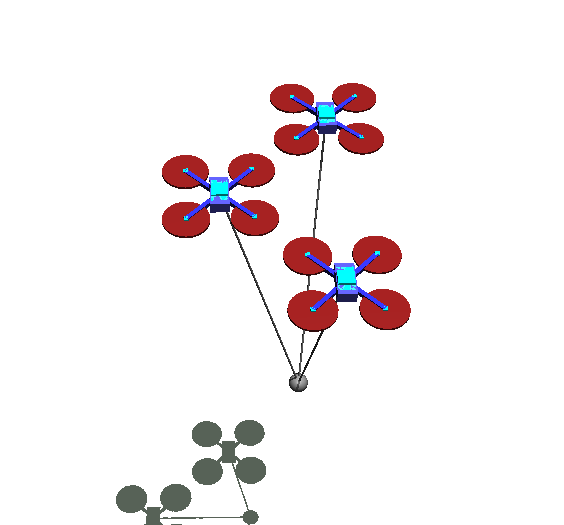
\includegraphics[width=34pc]{picture/5_3.png} 
	\caption{MuJoCo仿真引擎中的多无人机绳系吊运系统} 
	\label{5_3}
\end{figure}

为了增强仿真结果的可视化与交互,Mujoco 提供了与外部可视化工具(如 OpenGL)集成的能力,允许开发者实时观察仿真过程中的系统状态如图 \ref{5_3} 所示。这种高度交互性和可视化能力大大提升了开发者在测试和调试过程中的效率。

\begin{figure}[hbt!]
	\centering
	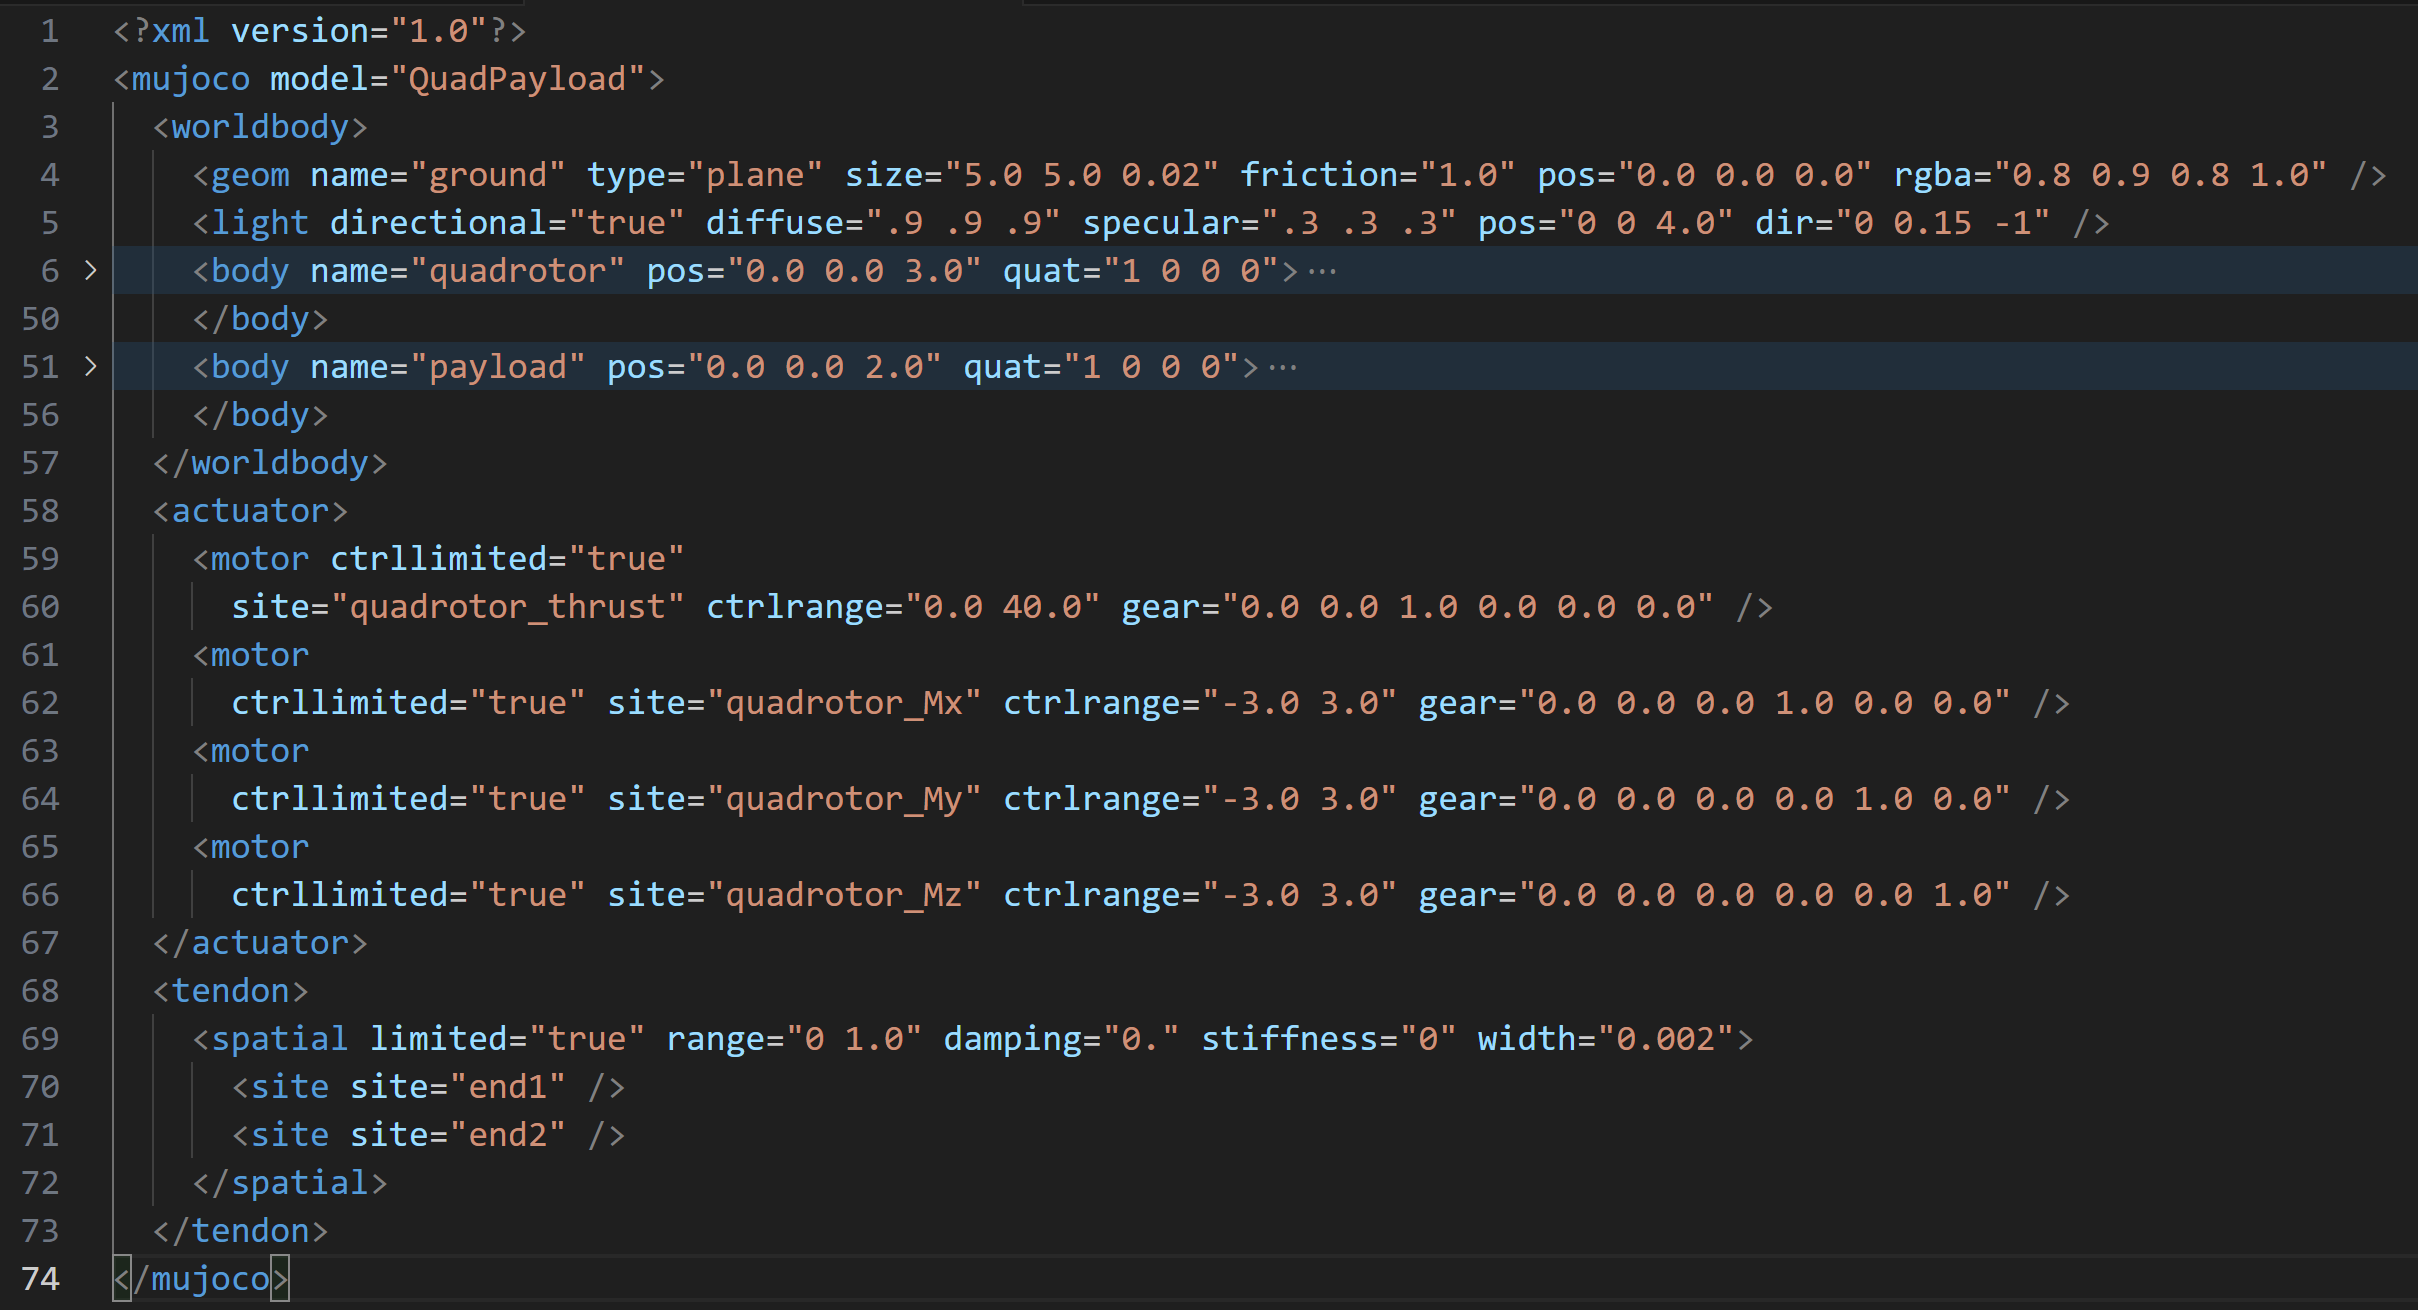
\includegraphics[width=36pc]{picture/MJCF.png} 
	\caption{无人机绳系吊运系统的 MJCF文件} 
	\label{MJCF}
\end{figure}
MJCF(MuJoCo XML Format)是 MuJoCo 仿真引擎中用于定义系统模型的标准化文件格式。与 SDF 文件不同,MJCF 文件在描述机器人结构时不是用父节点和子节点的方式,而是通过直接的嵌套表示其父子关系。MJCF不仅能表示机器人本体信息,还能表示环境信息,其主体并不是系统本身,而是整个世界,里面可以可嵌套多个系统。

如图 \ref{MJCF} 所示,MJCF文件采用 XML 语法,通过详细描述多体系统的各个组成部分,定义物理世界中物体的几何形状、动力学属性、约束条件、接触模型等,是 MuJoCo 中建模与仿真任务的核心工具之一,为仿真引擎提供了一种灵活且易于扩展的方式来描述复杂的动力学系统。MuJoCo 中的 tendon 组件提供了一种强大而灵活的方式来模拟柔性组件,尤其适用于模拟系绳等系统。通过设置拉伸刚度、阻尼以及连接的关节,tendon 组件能够有效地将柔性动力学融入到刚体动力学仿真中,为复杂系统建模提供了极大的便利。


\section{无人机绳系吊运系统控制仿真验证}
\subsection{动力学与环境模型的构建}
在仿真平台中,首先对四旋翼无人机及其绳系吊运系统进行动力学建模,包括无人机主体的刚体模型、旋翼的气动力模型,以及绳系的柔性力学模型。接着,在环境建模中引入以下关键要素:

绳系的约束建模:模拟系绳在受力、摆动及碰撞等情况下的动力学行为。
外部环境扰动:包括风场、气流湍动等干扰因素,用以测试控制算法的鲁棒性。
目标物体:模拟无人机需吊运的目标物体,其质量、重心及几何特性对吊运系统的稳定性影响显著。
\subsection{仿真系统的功能验证与优化}
在完成模型构建后,通过对以下典型任务场景的仿真,验证系统的功能及性能:

轨迹跟踪:设定预定轨迹,测试无人机在不同载荷条件下的轨迹跟踪能力及控制精度。
抗干扰能力:施加随机扰动,评估无人机对环境变化的响应特性。
稳定性分析:在复杂任务环境中,模拟绳系摆动的动态特性,验证算法的适用性与稳定性。
通过对上述平台的综合使用和比对分析,仿真系统为后续试验验证及算法优化提供了可靠的基础和参考数据。

\subsection{单无人机吊运仿真验证}


\subsection{多无人机吊运仿真验证}

\section{试验系统介绍}


\subsection{硬件配置}
\begin{figure}[hbt!]
	\centering
	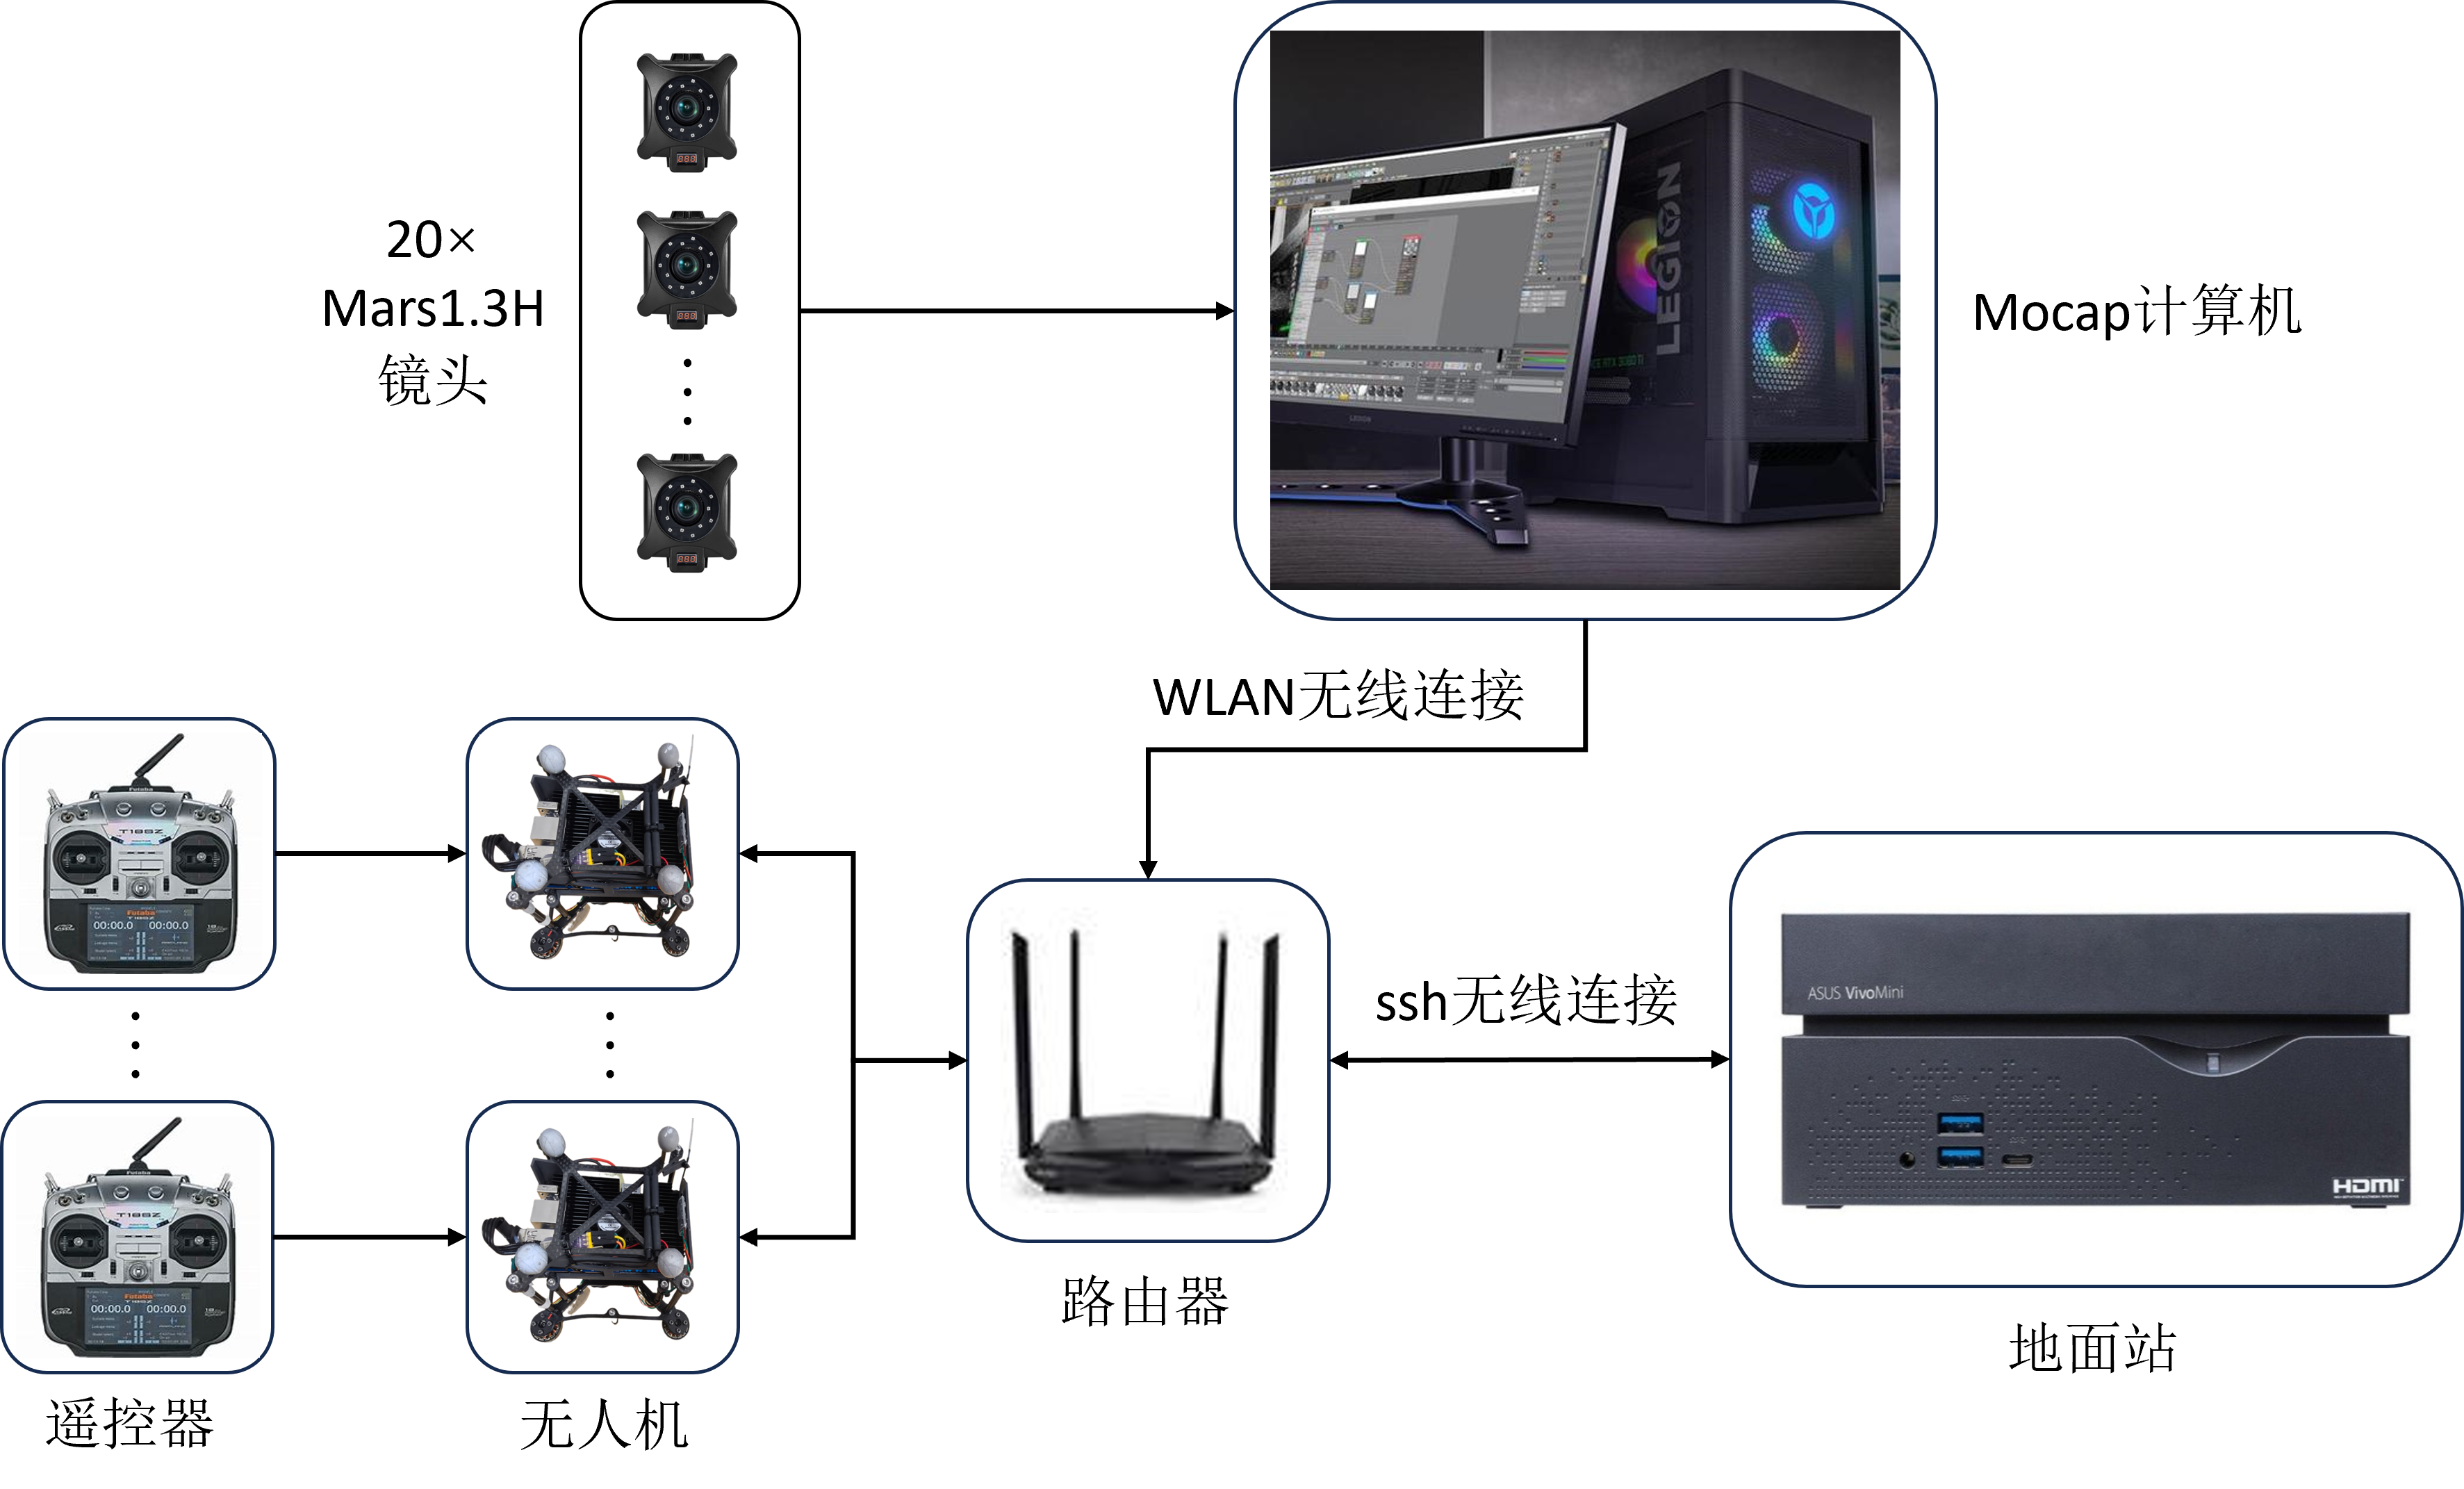
\includegraphics[width=36pc]{picture/5_4.png} 
	\caption{室内试验系统硬件配置} 
	\label{framework}
\end{figure}
由于无人机吊运控制算法在实机测试中需要精确获取自身位置,而室外环境受地形复杂、信号干扰及气候条件等因素的限制,难以实现高精度的绝对位置测量。为此,试验选择在室内环境开展测试,采用动作捕捉设备进行无人机位置的测定。动作捕捉设备通过高精度相机阵列实时跟踪目标,能够
提供亚毫米级的精确位置数据,具有抗干扰能力强、稳定性高的特点,为算法的验证和性能评估提供了可靠的参考基准。整个系统的硬件框架如图 \ref{framework} 所示。


动作捕捉设备选用NOKOV(度量)光学三维动作捕捉系统,该系统采用20个高性能红外摄像头捕捉反光标识点,采集并生成精准、实时的动作信息,可广泛应用于无人机室内定位追踪、多智能体协同控制等领域。在无人机上安装四个非共面的反光标识点,并通过四个反射球创建一个刚体,动作捕捉设备能够高精度地解算出刚体的位姿,并提供亚毫米级精度的高频实时位姿估计。

机载计算设备与Mocap计算机通过局域网建立连接,Mocap计算机将解算得到的位姿信息通过路由器进行广播,无人机上的板载计算设备在接入路由器的局域网后使用VRPN协议可以获取得到广播的实时位姿信息。同时,地面站通过路由器的局域网ssh连接至无人机的机载计算机,可以对无人机发布控制命令并监控其自身状态。

无人机平台的硬件选择主要考虑了算力、重量及接口等因素。试验平台选用了Orange Pi 5开发板作为机载计算设备,如图 \ref{fig.fmtpath} 所示,Orange Pi 5配备了Rockchip RK3588S处理器,这是一款高性能八核 ARM Cortex-A76 和 Cortex-A55 的混合架构处理器,提供强大的CPU计算性能,同时支持 GPU 和 NPU 加速。此外,Orange Pi 5的薄型设计和轻巧重量使其能够轻松地安装在无人机上,同时提供了丰富的接口,适配多种外设。在下位机选择方面,无人机平台采用了香港科技大学-大疆创新科技联合实验室基于PX4开源项目开发的NxtPX4v2飞控系统,如图 \ref{fig.proximity-tra} 所示,该飞控采用了STM32H743VIH6主处理器和双BMI088 IMU冗余传感器组,设计迷你小巧,安装孔间距为标准的20*20mm,可以在大多数小型穿越机机架上安装,并在最大程度上保障飞行任务的执行。

\begin{figure*}[htb!]
    \centering
    \begin{minipage}[t]{0.96\textwidth}
        \centering
        \begin{subfigure}[t]{0.47\textwidth}
            \centering
            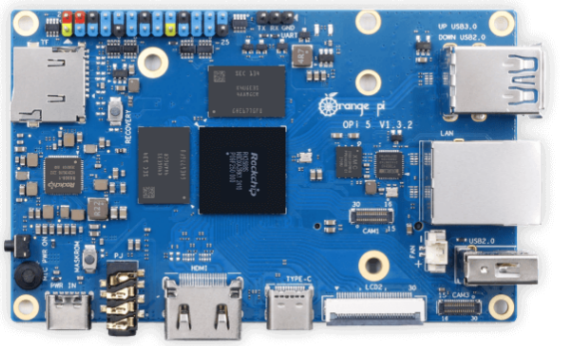
\includegraphics[height = 1.85in]{picture/5_5.png}
            \caption{Orange Pi 5开发板\label{fig.fmtpath}}
        \end{subfigure}\hfill
        \begin{subfigure}[t]{0.47\textwidth}
            \centering
            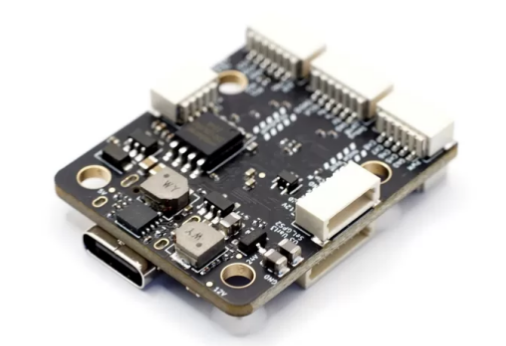
\includegraphics[height = 1.95in]{picture/5_6.png}
            \caption{NxtPX4v2飞控\label{fig.proximity-tra}}
        \end{subfigure}
    \end{minipage}
    \caption{无人机硬件控制系统}
\end{figure*}

% \begin{figure}[hbt!]
%     \centering
%     \begin{subfigure}[t]{0.45\textwidth}
%         \centering
%         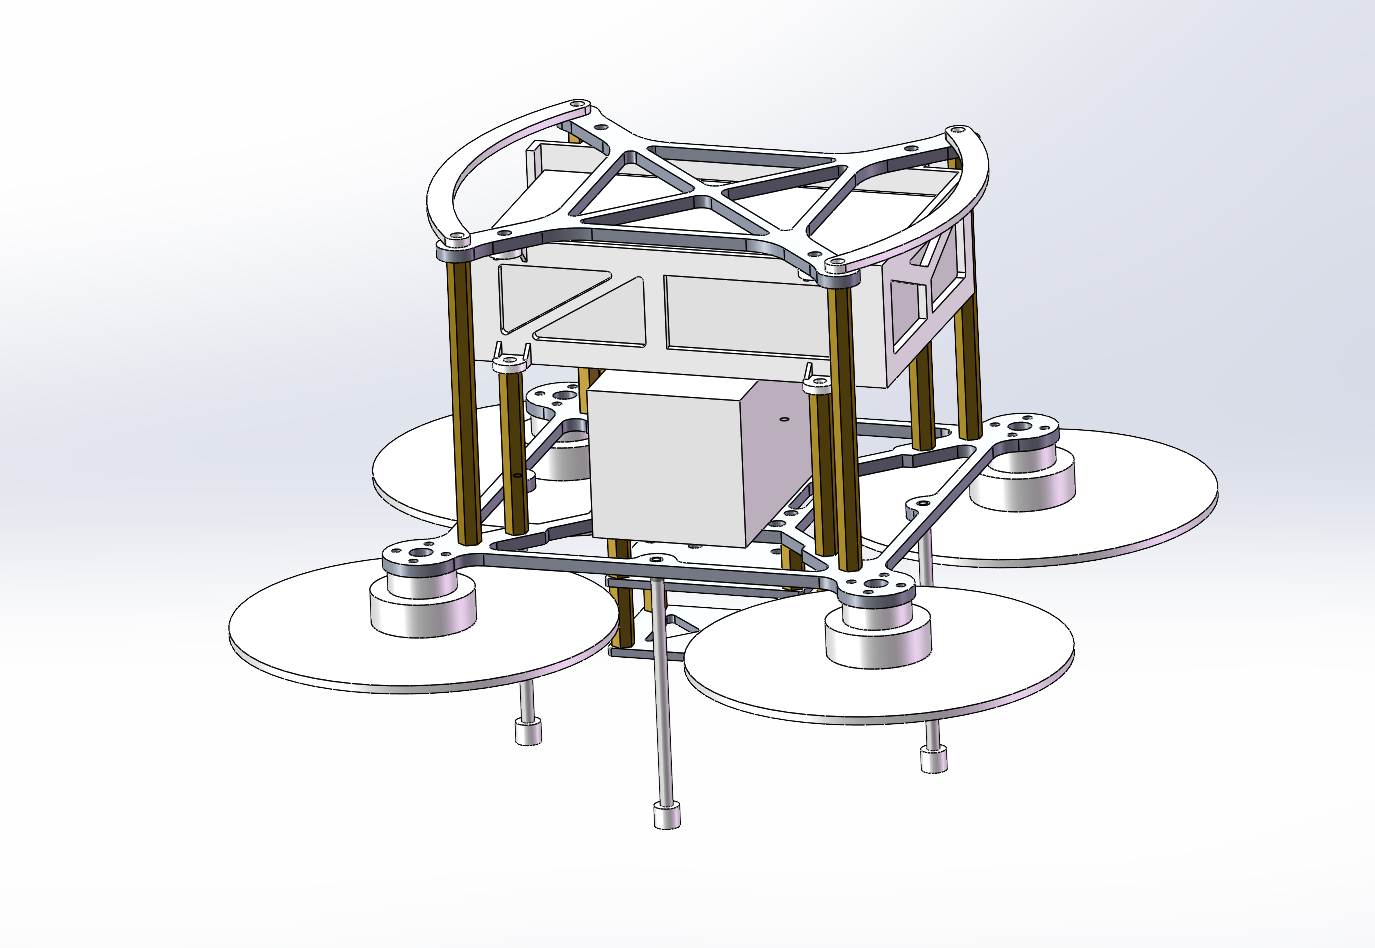
\includegraphics[width=\textwidth]{picture/5_7.png}
%         \caption{无人机为父节点}
%         \label{fig.fmtpath}
%     \end{subfigure}\hfill
%     \begin{subfigure}[t]{0.45\textwidth}
%         \centering
%         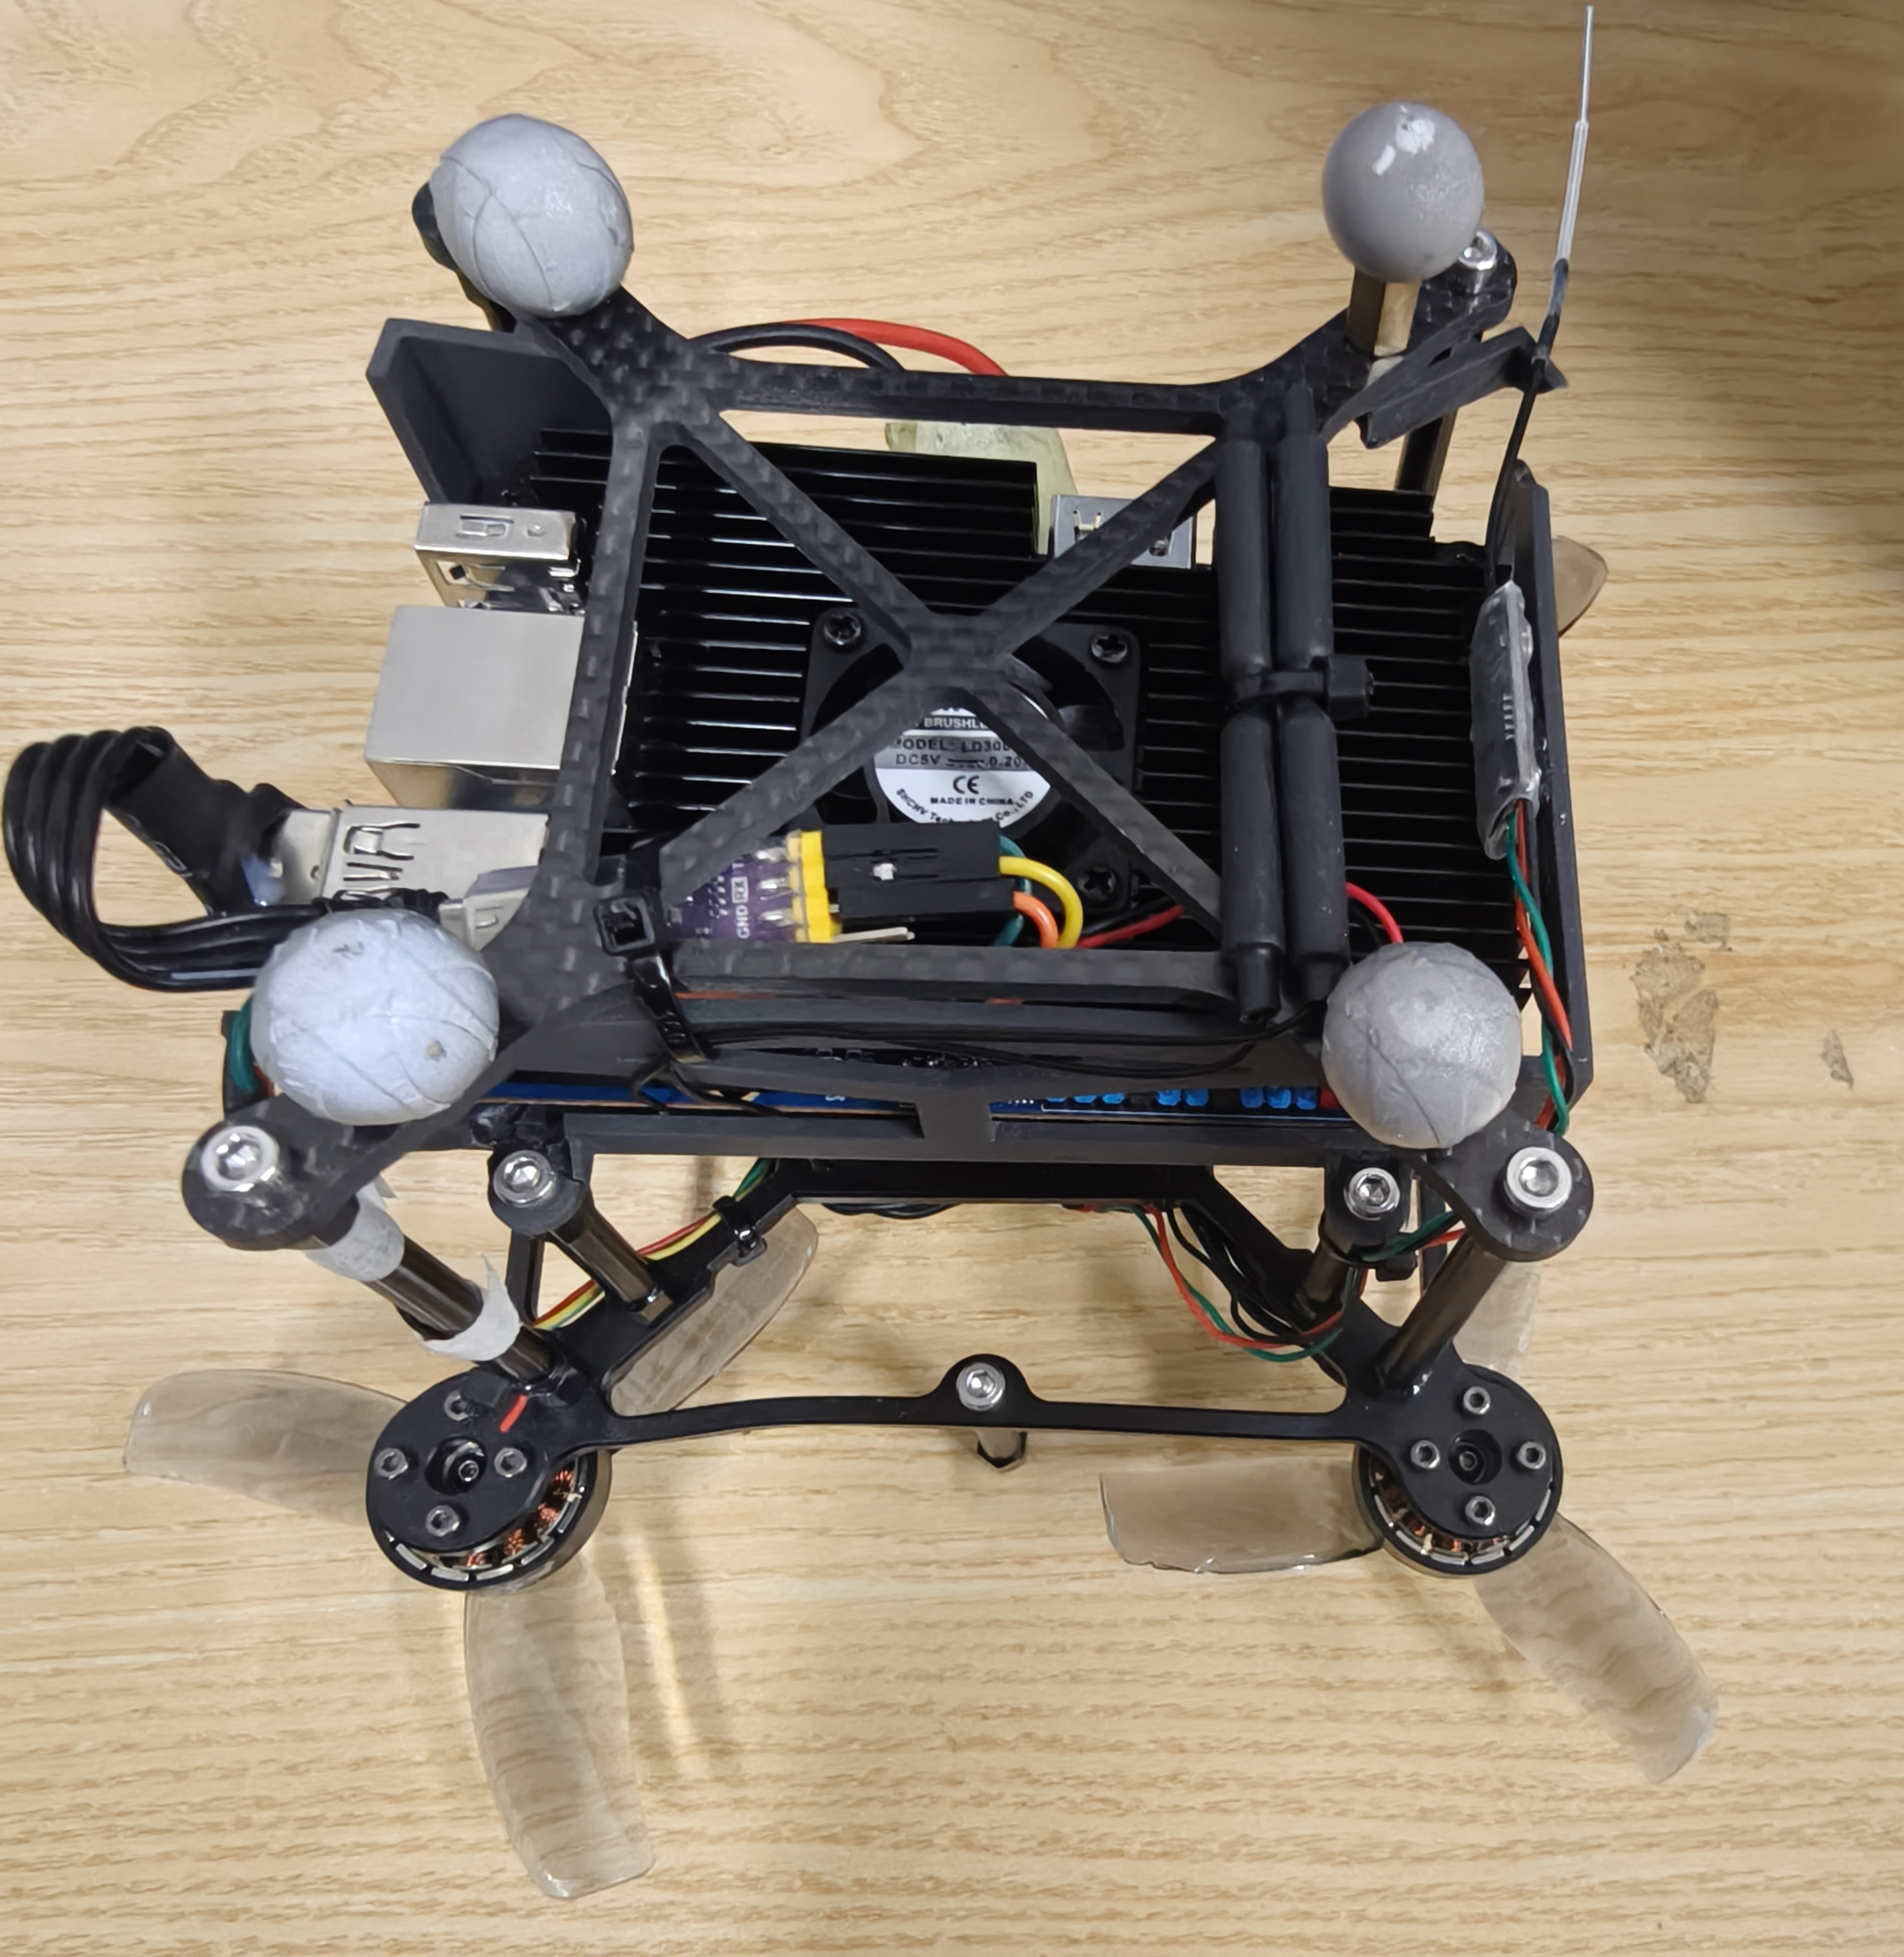
\includegraphics[width=\textwidth]{picture/5_8.png}
%         \caption{载荷为父节点}
%         \label{fig.proximity-tra}
%     \end{subfigure}
%     \caption{由无人机、系绳和载荷构成的树图}
%     \label{fig.proximity.kk}
% \end{figure}

在无人机平台的机械部分设计中,机架的选择至关重要,其决定了可以安装的最大桨叶尺寸、电池大小等。本文选择了自制的3.5寸机架,采用双层碳板结构的机臂和中心板,并通过铝柱连接,既轻便又具备较高的强度。为了充分利用空间使无人机的结构更加紧凑,机载计算设备置于机架顶部,下位机飞控和电子调速器置于机架底部,并用底层板保护,这样布局可以更好地对无人机的控制能力进行验证。在动力系统方面,电机选用了四个T-Motor F2004无刷电机,电子调速器采用蓝鸟48K 30A四合一电调,桨叶选用了两对QProp DT90自锁3叶正反尼龙桨,为无人机提供平稳、精准的动力输出。电池方面,选择了格氏金砖系列6s1p 1050mAh 95C锂电池组,相比于5s电池,6s电池提供更强的动力,可直接对Orange Pi 5供电,满载测试续航时间为6分钟,能够满足试验需求。定制的无人机重1.0 kg,电机轴距为360 mm。最后, 对其他的安装件位置进行设计,包括电池固定件、接收机、数传和降压模块等。最终得到无人机的设计图和实物图如图 \ref{Fig.proximity} 所示。
\begin{figure*}[htb!]
	\centering
	\begin{minipage}[t]{0.96\textwidth}
		\centering
		\begin{subfigure}[t]{0.47\textwidth}
			\centering
			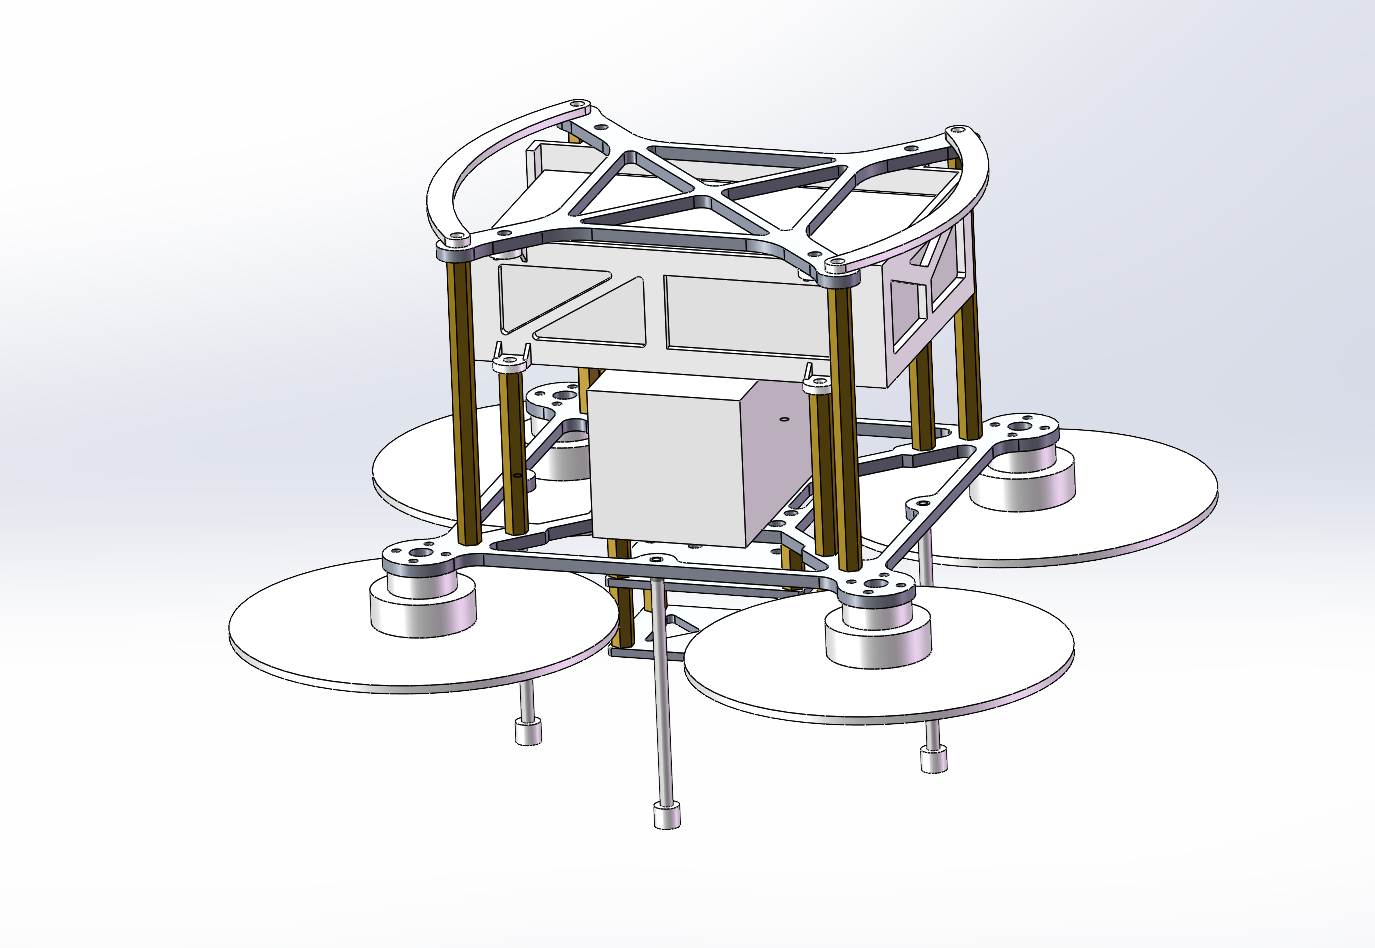
\includegraphics[height = 2.25in]{picture/5_7.jpg}
			\caption{SOLIDWORKS设计图\label{fig.path}}
		\end{subfigure}\hfill
		\begin{subfigure}[t]{0.47\textwidth}
			\centering
			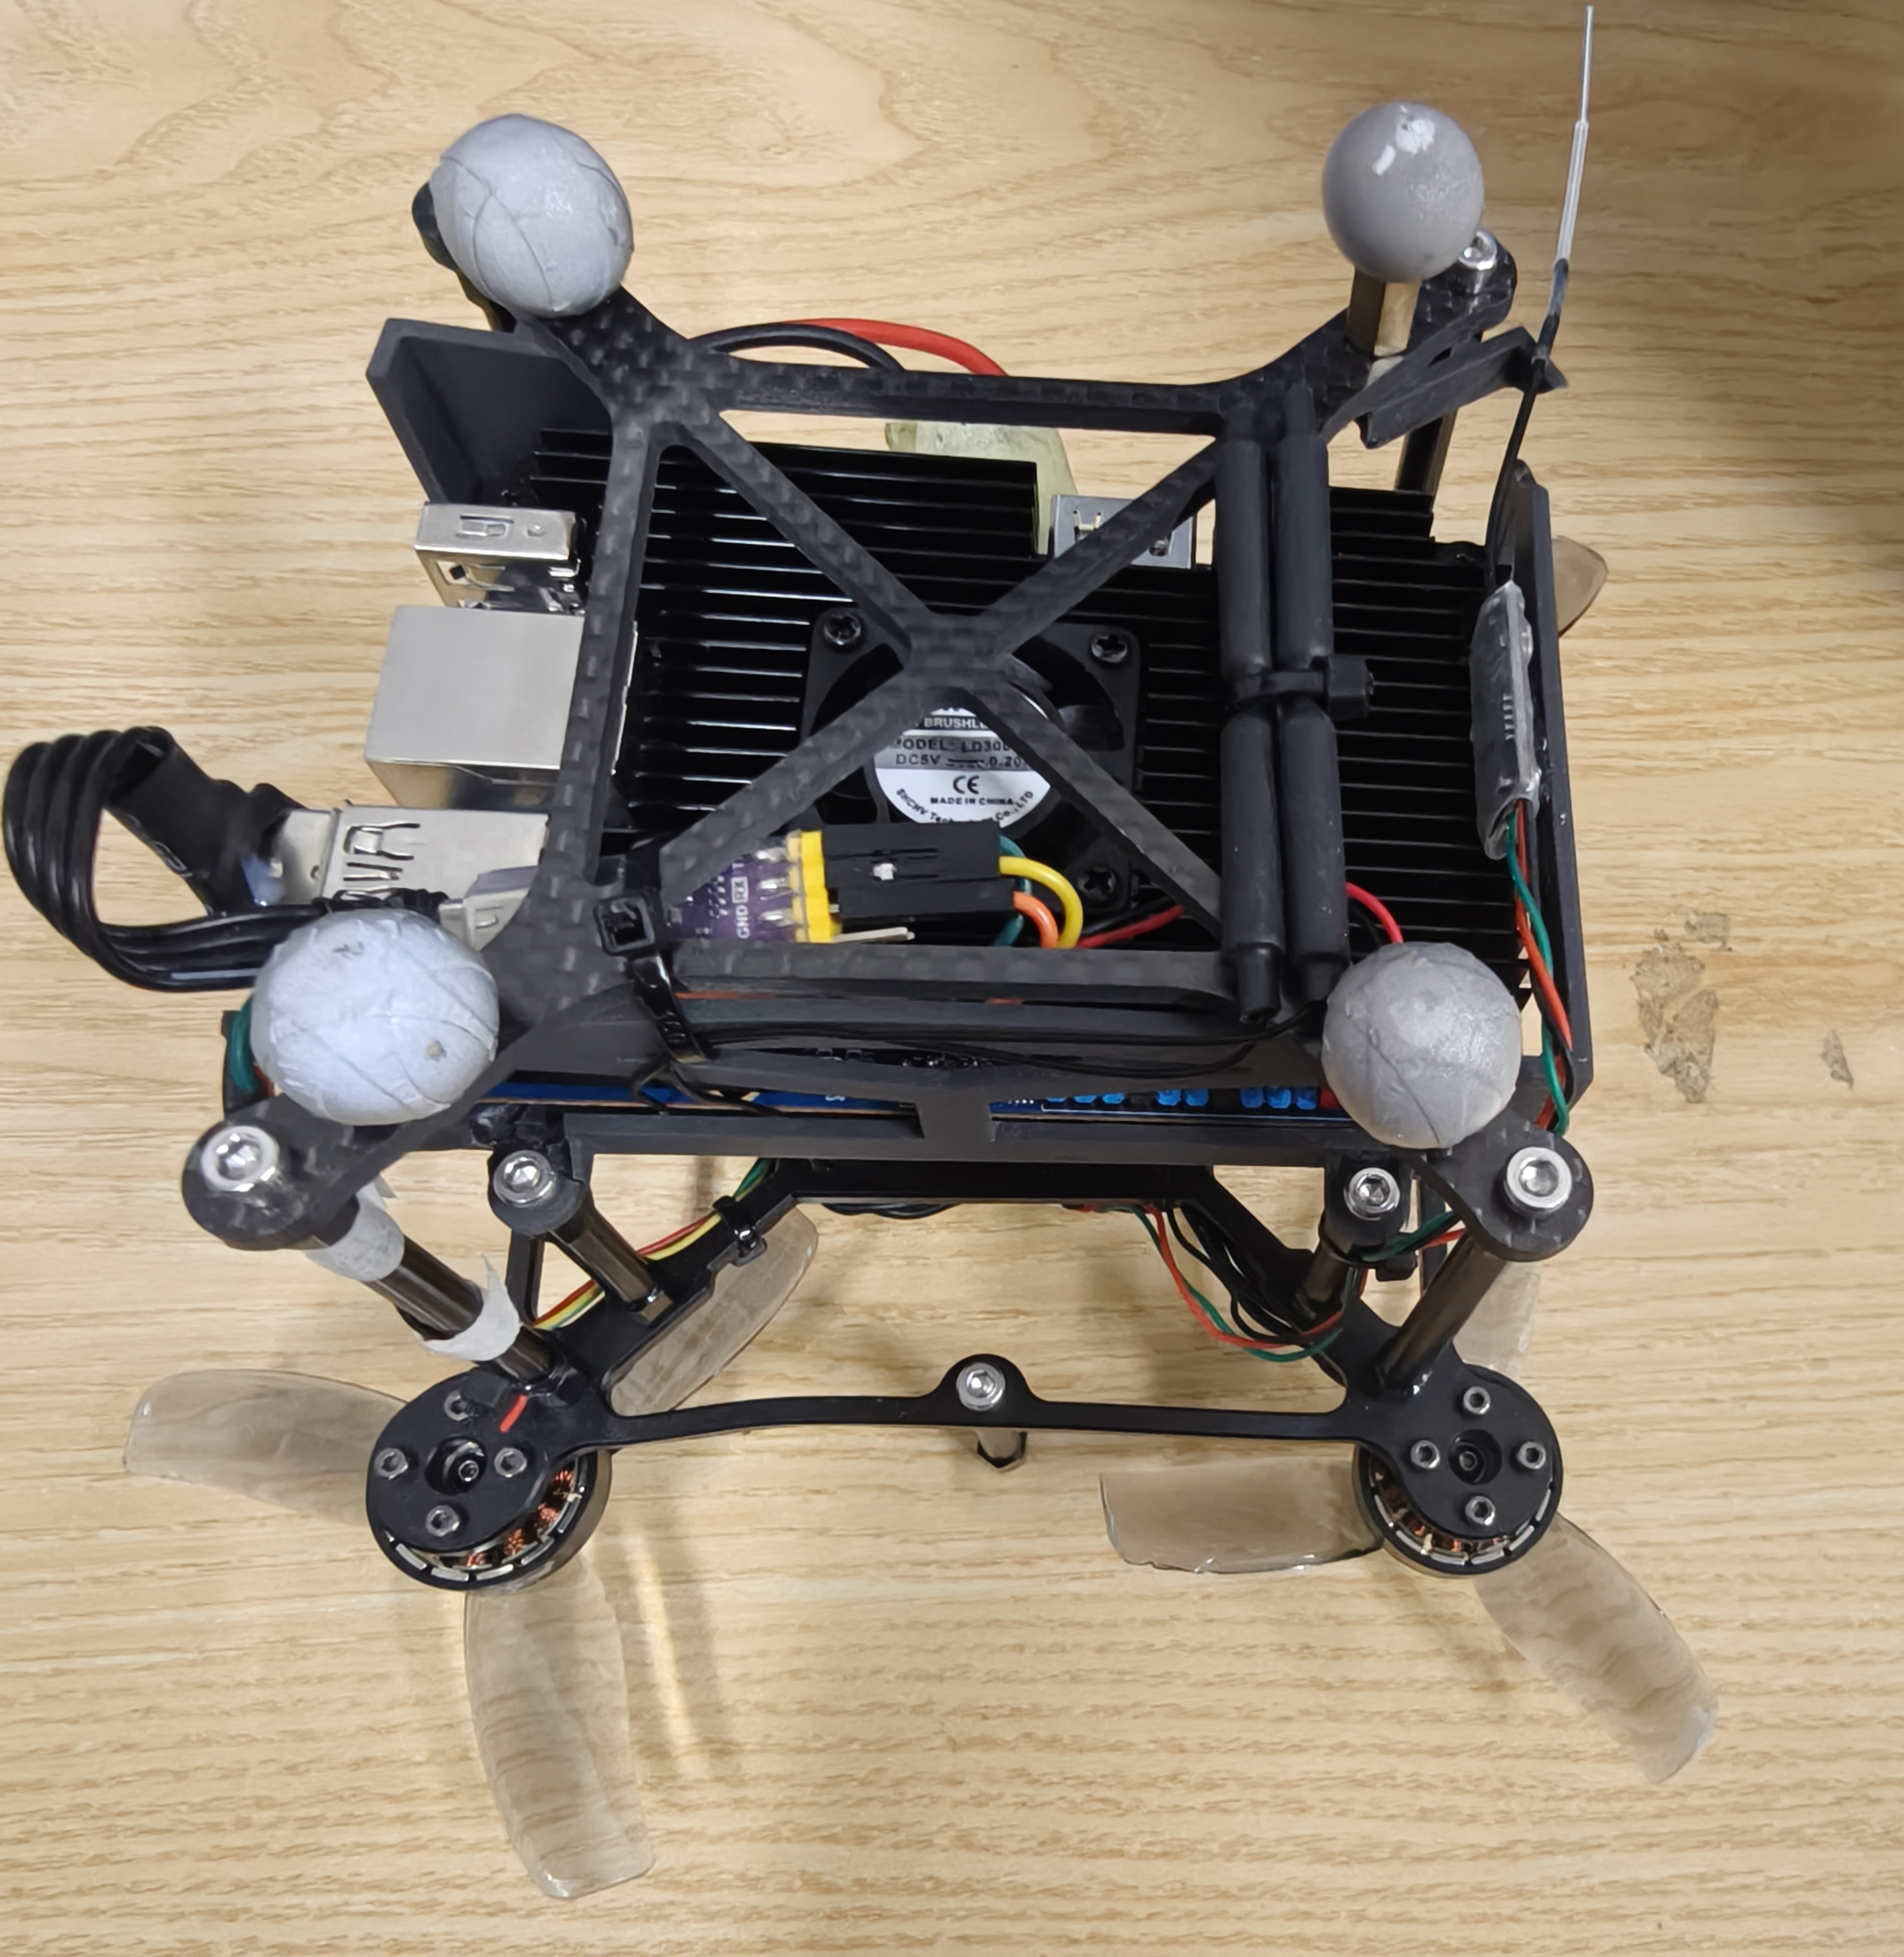
\includegraphics[height = 2.25in]{picture/5_8.jpg}
			\caption{实物图\label{fig.proximity}}
		\end{subfigure}
	\end{minipage}
	\caption{无人机平台设计图和实物图\label{Fig.proximity}}
\end{figure*}



\subsection{软件配置}
试验平台的软件环境为无人机绳系吊运系统在通信层提供支持,并提供了算法的运行等基本环境,所采用的算法基于 Ubuntu 22.04 和 ROS 2 Humble 进行部署。ROS 2 相较于 ROS 1 在多个关键方面展现出显著优势,显著提升了机器人软件开发的效率和系统性能。ROS 2 采用实时中间件 DDS,增强了系统的实时性和确定性,满足了高实时性应用的需求,其分布式架构和基于 DDS 的通信机制提升了系统的扩展性和多机器人协同能力,同时引入了身份认证和数据加密等安全特性,确保了数据传输的安全性。模块化设计和 colcon 包管理系统提高了系统的可扩展性和可维护性,现代化工具链如 rviz 2 简化了开发、测试和部署流程。此外,ROS 2 拥有活跃的社区和丰富的开源资源,众多开发者基于ROS 2开发应用,并将成熟的代码开源到社区中,促进了ROS 2生态系统的快速扩展。本文中,ROS 2通过基于colcon的构建和包管理方案、部分底层设备驱动、多线程管理以及进程间通信方案得以应用。

图 \ref{framewor} 展示了算法在试验过程中所使用的主要软件包及其间传递的消息内容。在实物试验中,动作捕捉设备以100Hz的频率提供外部绝对定位信息,并通过无线连接传递给飞控系统,与飞控系统中的传感器数据进行融合并作为源数据使用。
无人机控制程序采用C++语言编写,板载计算设备通过USB转串口线与飞控系统连接,通信波特率设置为921600。主程序首先定义了发送和接收的数据类型,涵盖了输出推力、姿态角、位置信息以及以四元数表示的姿态数据。控制算法由定时器以20毫秒的周期触发运行,计算结果通过 uXRCE-DDS 中间件传输至飞控系统以执行相应操作。
uXRCE-DDS(Micro XRCE-DDS) 是由 eProsima 开发的一种轻量级通信中间件,旨在为资源受限的嵌入式设备提供与标准 DDS(Data Distribution Service)生态系统的无缝集成。它基于 XRCE(eXtremely Resource Constrained Environments) 规范,专为微控制器和其他受限硬件环境设计,确保在低功耗和有限计算资源的设备上实现高效的实时数据分发和通信,这为 PX4 和 ROS 2 之间提供了快速可靠的集成,并使 ROS 2 更容易获取无人机自身信息以及发送指令,从而更精确地实现了无人机的控制和数据传输。
QGC地面站提供数据监控和指令功能,用于监控数据以及申请自主飞行模式(Offboard模式)。需要特别指出的是,尽管上位机也具备申请Offboard模式的功能,但为了确保实物试验的安全性,禁止通过上位机进行此类申请,自主模式的切换仅通过遥控器和地面站执行。
\begin{figure}[hbt!]
	\centering
	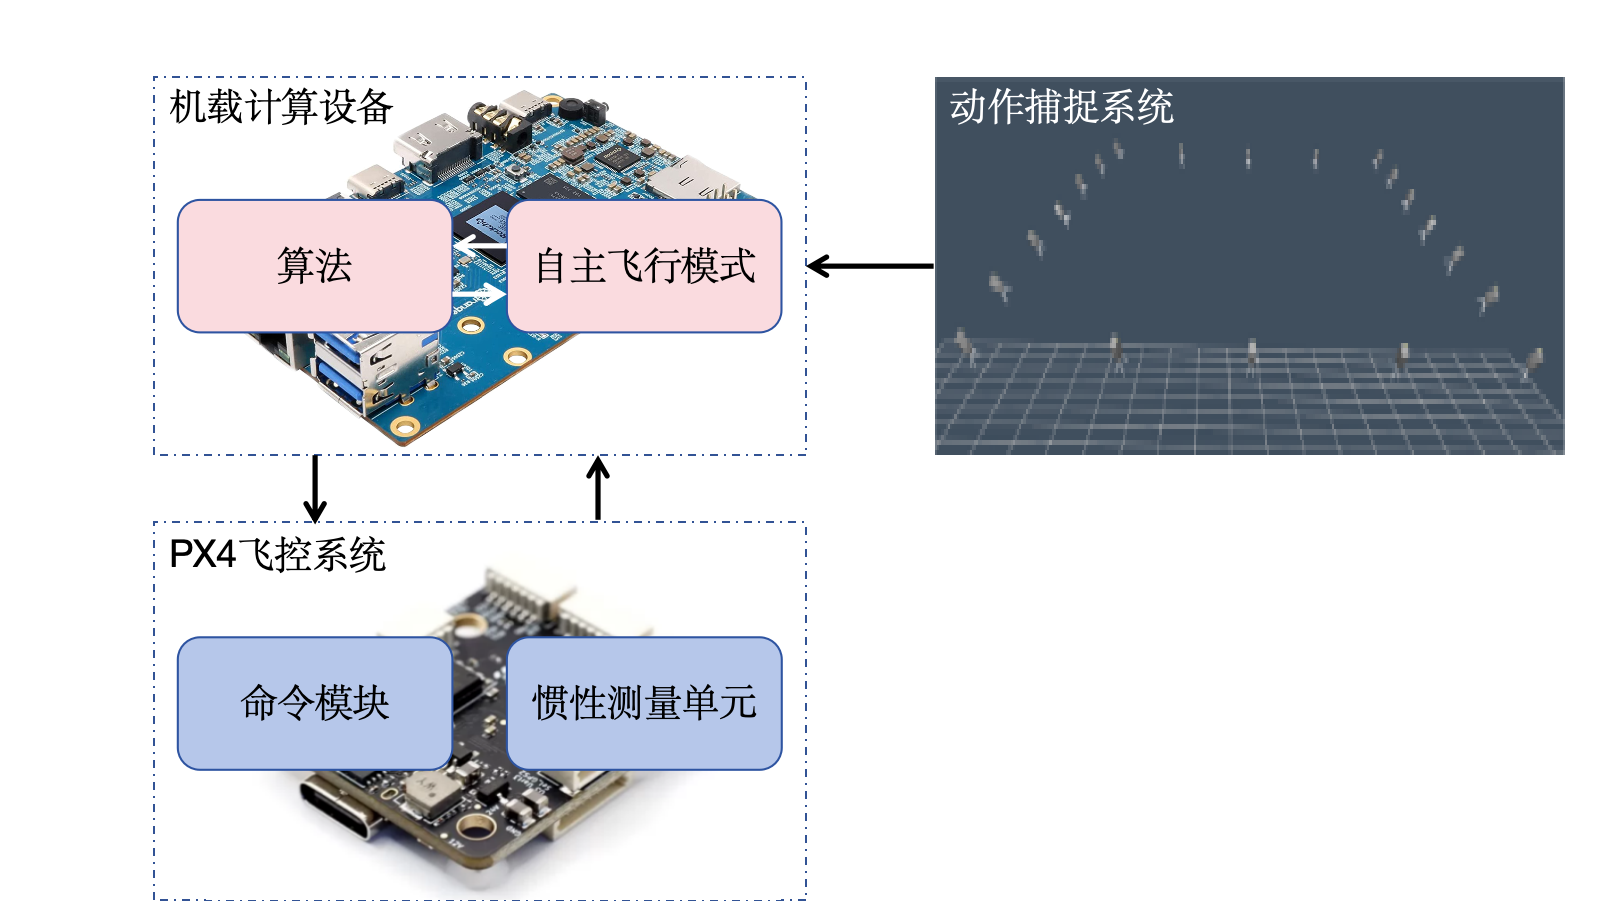
\includegraphics[width=38pc]{picture/5_9.png} 
	\caption{室内试验系统软件配置} 
	\label{framewor}
\end{figure}




% 系绳收放机构的软件部分使用C语言编程,设计包括主程序和子程序部分。主程序内初始化各个子模块,包括延时函数初始化、串口初始化、指示灯初始化以及定时器初
% 始化。子程序部分包括了定时器周期中断、张力传感器数据读取、伺服电机驱动和状态
% 反馈。当主程序完成各个子模块初始化后,便会循环进入定时器中断响应,一旦中断发
% 生,则立即响应中断请求执行相应任务。 
% 需要说明的是波特率是指每秒传送的字节数,读取张力传感器数据时串口的波特率
% 设置为9600,默认情况下驱动直流伺服电机时的波特率为57600。当主程序经过中断使
% 能后,定时器1ms中断一次,并以10ms的周期完成张力值读取、控制器运算和电机力
% 矩输出。为了检测程序实时运行情况,正常状态下板载LED灯每1s亮灭交替一次,如
% 发生程序堵塞,则LED灯出现状态异常。程序流程图如图5-12所示。 
% 60 
% 第5章  绳系无人机试验系统设计与试验验证 
% 中断开始
% 清除中断标志
% 10ms
% N
% Y
% 读取张力值
% N
% 控制器计算
% 控制伺服电机
% 转矩
% 1s
% Y
% LED灯亮灭交替
% 中断返回
% 图5-12 系绳收放机构软件逻辑 




\section{无人机绳系吊运系统控制试验验证}
\subsection{单无人机吊运试验验证}
如图 \ref{5_9} 所示,真实飞行实验的设置中,四旋翼配备了Pixhawk4用于姿态估计和低级别控制。四旋翼的位置和线性速度通过VICON运动捕捉系统进行估计。加速度和角速度则通过Pixhawk4的加速度计和陀螺仪传感器进行测量。所有优化问题(21)的求解实现均采用CasADi [21]和acados [22]进行部署。训练数据的采集频率为50 Hz,数据来源于基于圆形飞行轨迹的四旋翼系统,采用基线MPC控制器。训练集包含60秒的数据(3000个数据点),并通过公式(1)计算外部力和力矩作为标签,用于学习过程。数据采集实验中的系绳长度和载重分别为0.8 m和160 g,这些参数在所提框架的管道中是未知的。

我们首先展示神经预测器(Neural Predictor)在准确预测外部力方面的能力。在带有260 g载荷、悬停高度为1.6 m时,向系绳附加一个100 g的额外载荷。外部力预测结果如图 \ref{force} 所示。从结果可以看出,神经预测器对外部力变化的动态响应几乎是即时的。当载荷增加100 g时,神经预测器的输出增加了0.96 N,标准差为0.004 N。值得注意的是,由于存在残余动态,神经预测器的输出变化并不完全等于附加载荷的重力变化。这些结果表明,神经预测器能够准确且实时地估计外部力,并且能够适应不同的未知载荷。

\begin{figure}[hbt!]
	\centering
	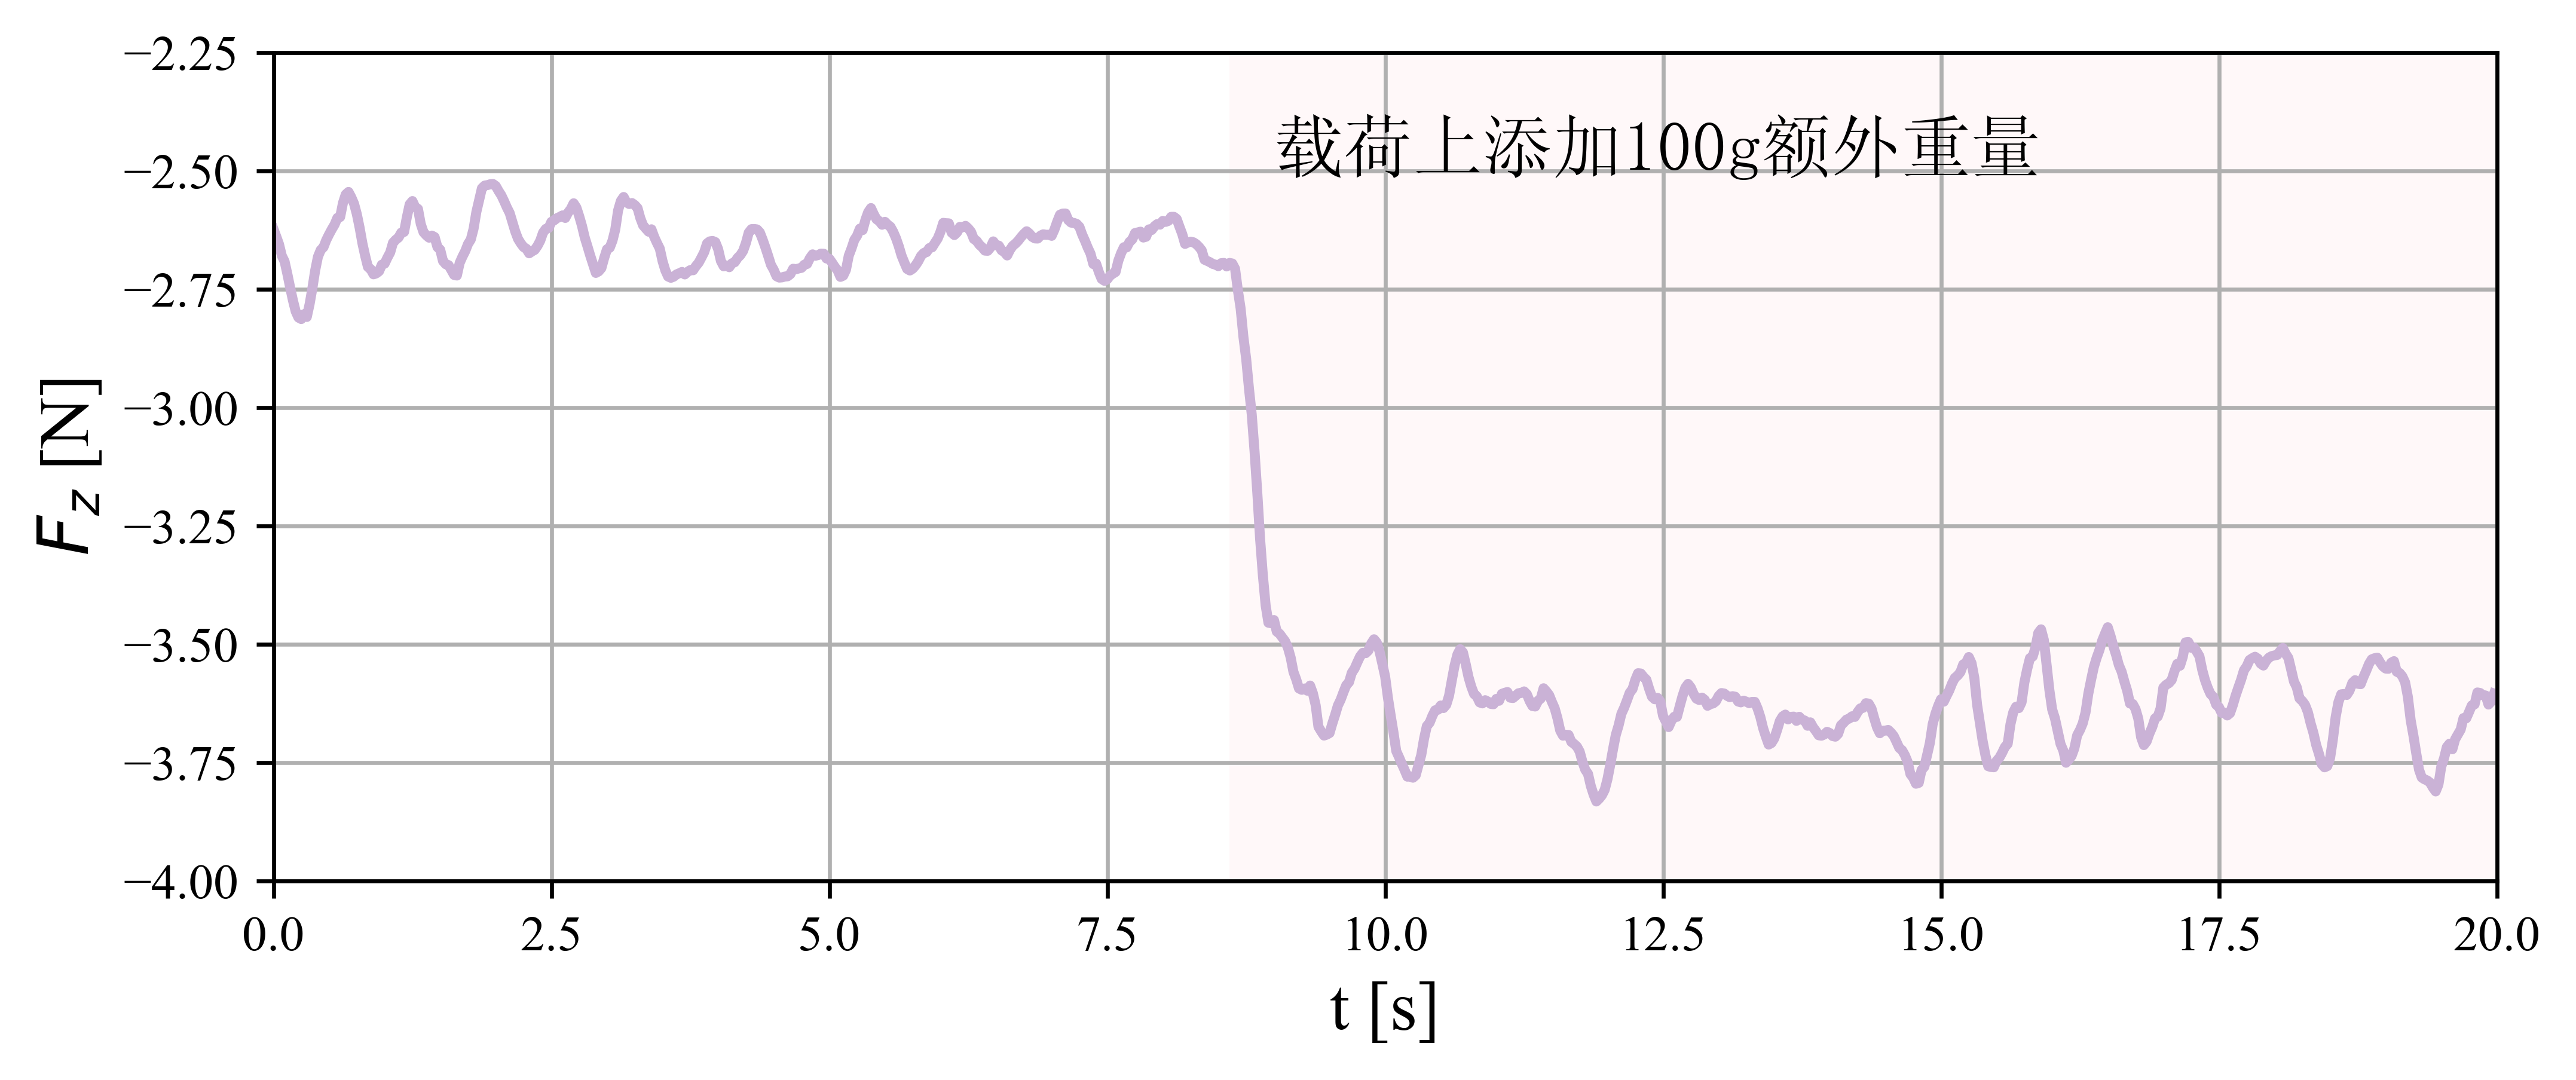
\includegraphics[width=38pc]{picture/kk/force.png} 
	\caption{在载荷上添加额外重量时Z轴方向外力的估算结果} 
	\label{force}
\end{figure}
接下来,进行了实际飞行中的轨迹跟踪实验,以验证NPMPC在轨迹跟踪方面的优越性,并与标准MPC以及其他两种相似框架(GP-MPC [11] 和 KNODE-MPC [12])进行比较。为了公平比较,三种学习型框架的训练集均来自上述数据采集实验中的60秒圆形轨迹。KNODE网络模型的架构与提升函数Φ相同。GP模型使用径向基函数(RBF)作为核函数,采用100个数据点,按照规则间隔进行采样并用于训练。NP、GP和KNODE模型的输入均为四旋翼的线性和角速度,正如我们在数值评估中所做的那样。参考信号由多项式轨迹生成器产生,参考高度为1.6 m,载荷重160 g。

四种框架在跟踪持续50秒的两条轨迹时的性能结果如表II和图 \ref{color} 所示。值得注意的是,由于载荷引起的建模不匹配,标准MPC在X-Y平面和Z轴的轨迹跟踪误差显著。而所有三种学习型框架(GP-MPC、KNODE-MPC和NP-MPC)通过数据捕捉到载荷引起的外部力,从而在跟踪误差上相较于标准MPC有所减少。在圆形轨迹跟踪实验中,GP-MPC、KNODE-MPC和NP-MPC都表现得比标准MPC更好,因为它们从数据中学习到建模不匹配并对MPC框架进行了补偿。然而,我们提出的NP-MPC在X-Y平面减少了53.45\%的跟踪误差,在Z轴减少了67.45\%,相较于标准MPC表现更为出色。在莱姆尼斯卡轨迹跟踪实验中,GP-MPC、KNODE-MPC和NP-MPC的跟踪表现也优于标准MPC。然而,当参考轨迹的曲率半径较小时,GP-MPC和KNODE-MPC的跟踪误差较大。需要注意的是,莱姆尼斯卡轨迹在几何上与训练集中的圆形轨迹有所不同。我们的NP-MPC能够在曲率半径较小时,仍然精确地跟踪参考轨迹。此外,在莱姆尼斯卡轨迹跟踪实验中,NP-MPC在X-Y平面减少了58.16\%的跟踪误差,在Z轴减少了76.72\%,相较于标准MPC。

\begin{figure}[hbt!]
	\centering
	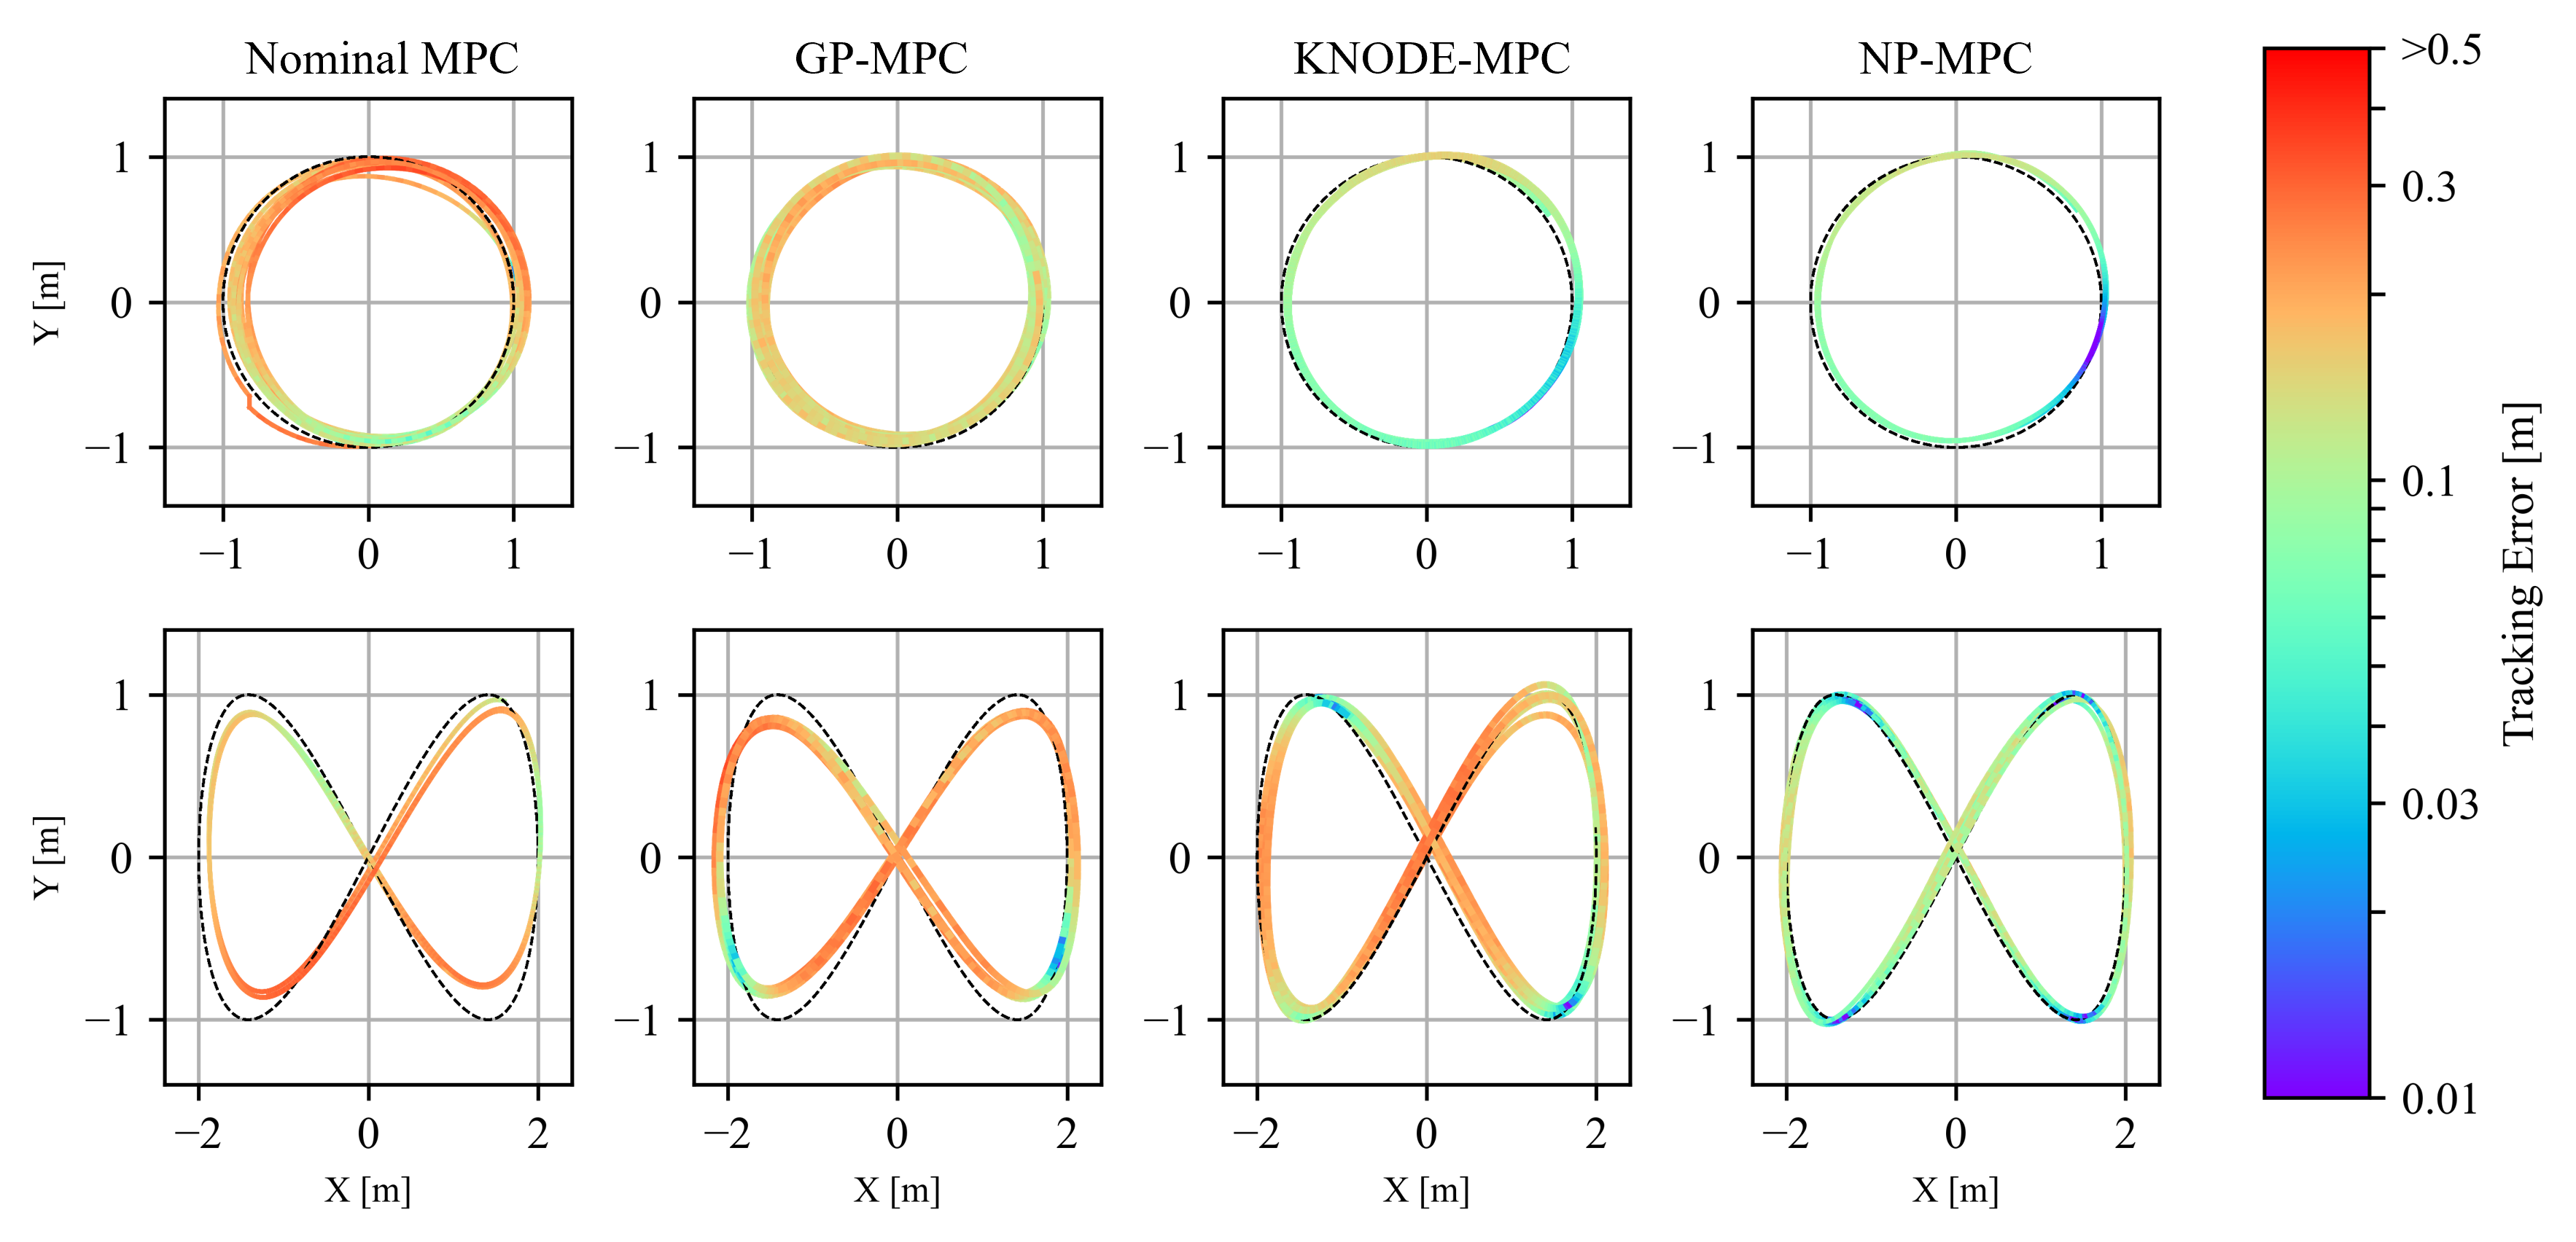
\includegraphics[width=38pc]{picture/kk/color.png} 
	\caption{在载荷上添加额外重量时Z轴方向外力的估算结果} 
	\label{color}
\end{figure}

为了验证神经预测器的泛化性能,可以使用训练数据集之外的速度数据和有效载荷质量进行测试。本实验考虑了四种测试场景。从第一个场景中收集数据集,并在此数据集上训练神经网络。 然后,设计了三种情况,即第二种情况改变速度大小,第三种情况改变半径大小,最后一种情况为有效载荷增加额外权重,以验证所提方法的泛化能力。图 \ref{prediction_res} 分别测试了不同速度、半径和有效载荷的情况。由于 PID 会导致跟踪延迟,因此这里没有绘制其轨迹。很明显,在所有情况下,与神经预测器合作的 NMPC 都比没有神经预测器的 NMPC 性能优越。跟踪性能最高提高了 65.1\%。特别是当有效载荷上附加了额外重量时,神经预测器凭借其快速响应能力可以迅速预测,从而使跟踪精度提高了 76.39\%。各种案例的结果表明,神经预测器对训练数据集领域之外的未见数据具有很强的泛化能力。
\begin{figure}[hbt!]
	\centering
	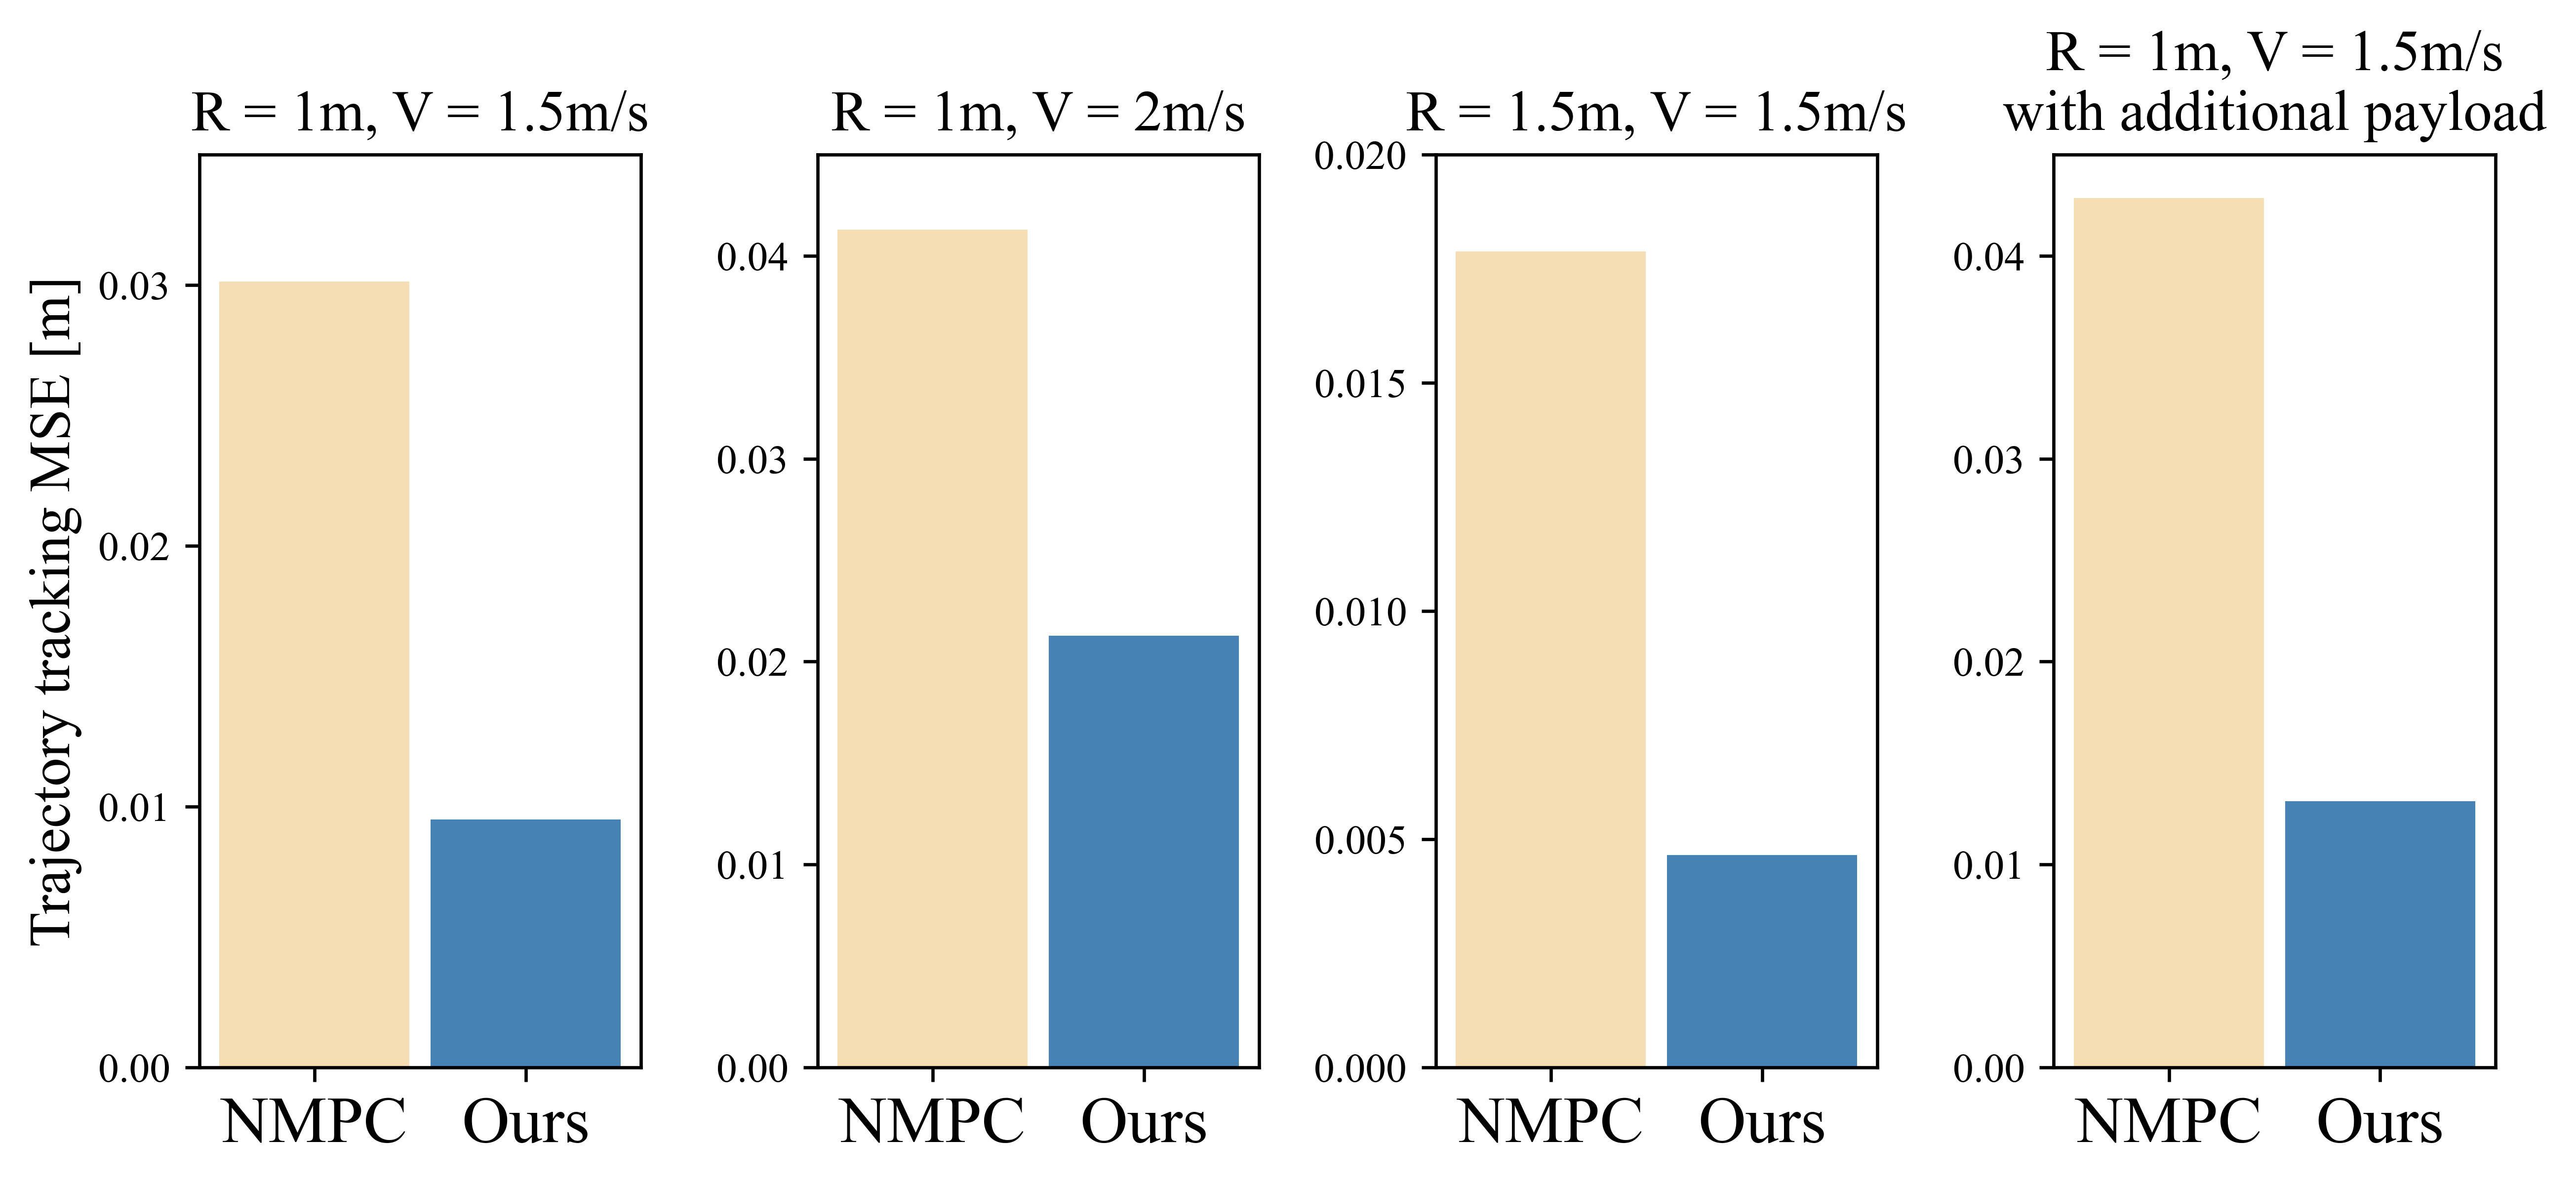
\includegraphics[width=38pc]{picture/kk/prediction_res.png} 
	\caption{在载荷上添加额外重量时Z轴方向外力的估算结果} 
	\label{prediction_res}
\end{figure}

综上所述,真实飞行实验结果表明:(1) 进一步验证了提出的神经预测器具有快速响应、准确估计和强大的泛化能力。(2) 神经预测器与MPC结合后,能够显著提高轨迹跟踪性能,优于其他类似框架。

\subsection{多无人机吊运试验验证}

\section{本章总结}


\cleardoublepage

\chapter{总结与展望}
\chaptermark{总结与展望}


\section{本文工作总结}


\section{未来工作展望}




%%=============================================================================%
%% 参考文献以及附录
%%-----------------------------------------------------------------------------%
\bibliographystyle{nputhesis}                               % GB/T 7714-2015 格式
%\bibliographystyle{nputhesis-noslash}                       % 参考文献改进格式
\bibliography{reference}                                    % 参考文献
%%=============================================================================%
%% 文档附页部分(致谢、参加科研情况、知识产权与原创性声明)
%%-----------------------------------------------------------------------------%
\backmatter                                                 % 文档附页部分
%%-----------------------------------------------------------------------------%
%\bibliography{ref}

\begin{acknowledgements}                                    % 致谢开始
时光如白驹过隙,转眼间我的研究生生活即将画上句号。在西北工业大学航天学院的三年求学岁月里,我不仅收获了专业知识,锻炼了科研能力,更收获了无数宝贵的友情和深厚的师生情谊。在此,我怀着感恩的心情,衷心感谢所有在我的成长过程中给予帮助、支持和鼓励的每一位老师、同学和家人。

首先,我要衷心感谢我的导师张帆教授。张老师严谨的治学态度和孜孜不倦的工作精神一直是我学习的榜样。作为我的导师,张老师不仅在学术上给予我无微不至的指导,还为我提供了优越的科研条件,并始终关心和支持我的成长。在张老师的教诲和引导下,我不断完善自己的专业技能,逐步迈向科研的高峰。在此,向张老师表达我最深的感激之情。

其次,我要感谢张帆老师,张老师的支持与鼓励在我的研究生生涯中占据了重要的位置。她不仅是我的学术导师,更像是我亲切的大姐姐。无论是在课题的设计、实施过程中,还是在面对困惑和挫折时,张帆老师始终给予我极大的关怀和帮助。她总是耐心地为我解答问题,鼓励我在科研上不断突破自我,从不因困难而气馁。我深深感激张帆老师对我个人成长的悉心帮助与关爱。


最深沉的感激,属于我的父母。感谢他们一直以来对我的无私支持和鼓励。无论是生活中的点滴关怀,还是学业上的悉心照顾,父母为我提供了坚强的后盾。正是因为他们的辛勤付出和无怨无悔的奉献,才让我能够在求学的道路上无所畏惧、勇往直前。父母的恩情,我将铭刻一生,终身难忘。

在学术和生活上,我还要感谢王通师兄、刘习尧师兄、刘亚师姐。感谢你们在我遇到学术难题时耐心的解答和指导。你们不仅帮助我解决了实验中的技术问题,也让我在学术研究中不断完善自我。还要特别感谢我的同门杨立、文思捷和师弟金澳,感谢你们在我的实验研究过程中提供的宝贵意见和支持,帮助我克服了诸多技术和设计难题。

此外,我的室友、老大哥粟刚,是我研究生期间的另一位重要人物。感谢你在我忙碌的学术生活中,给予我生活上的关心与支持。你的乐观与积极,深深感染了我,带我领略了西安的风土人情,品尝了无数美食,让我在繁重的课业中,依然保持了热情与动力。

我还要感谢课题组的各位老师:马志强老师、常海涛老师、刘星老师、沈刚辉老师、张夷斋老师、刘正雄老师,感谢你们在科研工作中的指导和帮助。你们的经验和建议让我在科学研究的道路上少走了许多弯路。还要感谢韩冬、陈海飞、黄冰潇、李陇南、李沅澔、赵亚坤、王志祥、宋梦实、张校祯、余航、高家乐、裴崇旭、翟晨萌、杨通等师兄师姐,感谢你们在学术上和生活中给予的帮助与关怀,让我的研究生生活更加丰富多彩。

再次感谢所有在我求学旅程中给予过帮助的人。你们的支持与鼓励,是我不断前行的不竭动力。未来的路上,我将继续努力,不忘初心,勇敢追求更高的目标。
\end{acknowledgements}                                      % 致谢结束
%%-----------------------------------------------------------------------------%
\begin{accomplishments}                                     % 参加科研情况开始
	论文发表情况
	\begin{enumerate}
		\item \blackbox{Ao Jin}, \blackbox{Chenhao Li}, \blackbox{Ya Liu}, \blackbox{Panfeng Huang} and \blackbox{Fan Zhang}. Neural Predictor for Flight Control with Payload [J].  IEEE Robotics
		and Automation Letters, 2024(中科院SCI 计算机科学类2 区, IF=4.6, 一审中)
	\end{enumerate}

    专利申请情况:
    \begin{enumerate}
    	\item \blackbox{张帆}, \blackbox{李晨豪}等. 一种柔性约束多智能体系统的协同运输鲁棒控制方法(发明专利,申请号/专利号:2024112841675)
    \end{enumerate}
\end{accomplishments}                                       % 参加科研情况结束
%%-----------------------------------------------------------------------------%
\makestatement                                              % 知识产权与原创性声明
%%=============================================================================%
%% 文档结束
%%-----------------------------------------------------------------------------%
\end{document}
%%=============================================================================%


%% 
%% This work consists of the file  yanputhesis.dtx
%% and the derived files           yanputhesis.ins,
%%                                 yanputhesis.pdf,
%%                                 yanputhesis.cls.
%% 
%%
%% End of file `yanputhesis-sample.tex'.
